\documentclass[a4paper,11pt]{article}
\usepackage{graphicx}
\usepackage[utf8]{inputenc} 
\usepackage{amsmath,amssymb,amsthm} 
\usepackage{booktabs}
\usepackage{hyperref}
\usepackage{longtable}
\usepackage{array}
\usepackage{float}
\usepackage{pdflscape}
\usepackage{microtype}   % nicer justification
\usepackage{caption}

\title{SI for \emph{Museum specimens reveal butterfly size increases through time but divergent responses to temperature}}
\author{Elsa Heywood,  Zoe M. Simmons,\\ J. Christopher D. Terry, Ailsa H. C. McLean}
\date{}

\begin{document}

\maketitle

\renewcommand{\thetable}{S1} % makes this table Table S1
\begin{landscape}
\section{SI Tables}

\footnotesize % shrink table text; change to \small or \scriptsize if needed
\setlength{\tabcolsep}{4pt} % reduce horizontal padding between columns
\renewcommand{\arraystretch}{1.05} % slightly tighter row spacing

\begin{longtable}{@{}
  >{\itshape}p{0.15\linewidth}  % Species (wraps)
  p{0.18\linewidth}  % Common Name (wraps)
  p{0.10\linewidth}  % Family
  p{0.05\linewidth}  % Habitat
  p{0.06\linewidth}  % Foodplant
  r                   % NHM_n (numeric, right-aligned)
  r                   % OUM_n (numeric, right-aligned)
  p{0.15\linewidth}  % Focal Brood (wraps)
  p{0.10\linewidth}  % FocalMonthLateLarval
  p{0.10\linewidth}  % GB Red List category
 @{}}

\caption{Details of butterfly species used in this study. Habitat and foodplant specialism status was split into two categories divided  specialists (S) and generalists (G). Numbers for each datasets are the post-filterring counts. See code repository for corresponding .csv file.}\\
\toprule
Species & Common Name & Family & Habitat & Foodplant & n (NHM) & n (OUMNH) & Focal Brood & Focal Month (Late Larval) & GB Red List category \\
\midrule
\endfirsthead

\multicolumn{10}{c}%
{\tablename\ \thetable\ -- \textit{Continued from previous page}}\\
\toprule
Species & Common Name & Family & Habitat & Foodplant & n (NHM) & n (OUMNH) & Focal Brood & Focal Month (Late Larval) & GB Red List category \\
\midrule
\endhead

\midrule
\multicolumn{10}{r}{\textit{Continued on next page}}\\
\endfoot

\bottomrule
\endlastfoot

Aglais urticae & Small tortoiseshell & Nymphalidae & G & S & 971 & 34 &1: Jun-Aug & May & Not Listed \\
Aricia agestis & Brown argus & Lycaenidae & S & S & 975 & 42 & 2:Aug-Oct & July & Not Listed \\
Celastrina argiolus & Holly blue & Lycaenidae & G & G & 303 & 25 & 2:Aug-Oct & June & Not Listed \\
Lasiommata megera & Wall & Nymphalidae & G & G & 619 & 62 & 2: Aug-Oct &June & Endangered \\
Leptidea sinapis & Wood White & Pieridae & S & S & 791 & 70 & 1: Mar-Jun& JulyBefore & Endangered \\
Lycaena phlaeas & Small copper & Lycaenidae & G & S & 2877 & 65 & 2:Jul-Oct & June & Not Listed \\
Pararge aegeria & Speckled wood & Nymphalidae & G & G & 471 & 38 & 2:Jul-Aug & June & Not Listed \\
Pieris brassicae & Large white & Pieridae & G & S & 344 & 44 & 2:Jul-Sep & June & Not Listed \\
Pieris napi & Green-veined white & Pieridae & G & G & 766 & NA & 2:Jul-Sep & June & Not Listed \\
Pieris rapae & Cabbage white & Pieridae & G & G & 445 & NA & 2: Jul-Sep& June & Not Listed \\
Polygonia c-album & Comma & Nymphalidae & G & G & 466 & 39 & 1: Jun-Aug& June & Not Listed \\
Polyommatus bellargus & Adonis Blue & Lycaenidae & S & S & 4830 & 63 &2: Aug-Sep & July & Vulnerable \\
Polyommatus icarus & Common blue & Lycaenidae & G & G & 3752 & 63 & 2:Aug-Sep & July & Not Listed \\
Aglais io & Peacock & Nymphalidae & G & S & 505 & 80 & Univoltine & June& Not Listed \\
Anthocharis cardamines & Orange tip & Pieridae & G & G & 1661 & 64 &Univoltine & JulyBefore & Not Listed \\
Apatura iris & Purple emperor & Nymphalidae & S & S & 124 & NA &Univoltine & March & Not Listed \\
Aphantopus hyperantus & Ringlet & Nymphalidae & G & G & 2206 & NA &Univoltine & June & Not Listed \\
Argynnis paphia & Silver washed fritillary & Nymphalidae & G & S & 1447& 83 & Univoltine & June & Not Listed \\
Boloria euphrosyne & Pearl-bordered Fritillary & Nymphalidae & G & S &1865 & NA & Univoltine & April & Vulnerable \\
Boloria selene & Small Pearl-bordered Fritillary & Nymphalidae & S & S &1925 & NA & Univoltine & April & Vulnerable \\
Callophrys rubi & Green hairstreak & Lycaenidae & G & G & 990 & NA &Univoltine & JuneBefore & Not Listed \\
Carterocephalus palaemon & Chequered Skipper & Hesperiidae & S & S & 604& NA & Univoltine & AugustBefore & Not Listed \\
Coenonympha pamphilus & Small Heath & Nymphalidae & G & S & 3058 & NA &Univoltine & April & Vulnerable \\
Coenonympha tullia & Large Heath & Nymphalidae & S & S & 1409 & 44 &Univoltine & April & Endangered \\
Cupido minimus & Small Blue & Lycaenidae & G & S & 1453 & 89 &Univoltine & JulyBefore & Near Threatened \\
Erynnis tages & Dingy skipper & Hesperiidae & G & S & 856 & 85 &Univoltine & AugustBefore & Not Listed \\
Euphydryas aurinia & Marsh Fritillary & Nymphalidae & G & S & 1926 & NA & Univoltine & May & Vulnerable \\
Fabriciana adippe & High Brown Fritillary & Nymphalidae & G & S & 994 &NA & Univoltine & May & Endangered \\
Favonius quercus & Purple hairstreak & Lycaenidae & G & S & 494 & 83 &Univoltine & May & Not Listed \\
Gonepteryx rhamni & Brimstone & Pieridae & G & S & 483 & 81 & Univoltine& June & Not Listed \\
Hamearis lucina & Duke of Burgundy & Riodinidae & S & S & 951 & NA &Univoltine & JulyBefore & Vulnerable \\
Hesperia comma & Silver-spotted Skipper & Hesperiidae & S & S & 646 &103 & Univoltine & June & Vulnerable \\
Hipparchia semele & Grayling & Nymphalidae & S & G & 1654 & NA &Univoltine & April & Endangered \\
Limenitis camilla & White Admiral & Nymphalidae & S & S & 761 & 97 &Univoltine & May & Vulnerable \\
Maniola jurtina & Meadow brown & Nymphalidae & G & G & 4730 & 70 &Univoltine & April & Not Listed \\
Melanargia galathea & Marbled white & Nymphalidae & G & G & 2169 & 101 &Univoltine & May & Not Listed \\
Melitaea athalia & Heath Fritillary & Nymphalidae & G & G & 1619 & NA &Univoltine & March & Endangered \\
Melitaea cinxia & Glanville Fritillary & Nymphalidae & S & S & 579 & NA& Univoltine & March & Endangered \\
Nymphalis polychloros & Large Tortoiseshell & Nymphalidae & G & G & 197& NA & Univoltine & June & Regionally Extinct \\
Ochlodes sylvanus & Large skipper & Hesperiidae & G & G & 1029 & NA &Univoltine & May & Not Listed \\
Papilio machaon & Swallowtail & Papilionidae & S & S & 166 & 54 &Univoltine & JulyBefore & Vulnerable \\
Plebejus argus & Silver-studded Blue & Lycaenidae & S & G & 7105 & NA &Univoltine & May & Vulnerable \\
Polyommatus coridon & Chalk Hill Blue & Lycaenidae & G & S & 19584 & NA& Univoltine & June & Vulnerable \\
Pyrgus malvae & Grizzled Skipper & Hesperiidae & G & G & 1285 & 108 &Univoltine & July & Vulnerable \\
Pyronia tithonus & Gatekeeper & Nymphalidae & G & S & 2313 & 125 &Univoltine & June & Not Listed \\
Satyrium pruni & Black Hairstreak & Lycaenidae & S & S & 377 & NA &Univoltine & May & Endangered \\
Satyrium w-album & White-letter Hairstreak & Lycaenidae & S & S & 346 &NA & Univoltine & May & Vulnerable \\
Speyeria aglaja & Dark Green Fritillary & Nymphalidae & G & S & 1028 &51 & Univoltine & May & Near Threatened \\
Thecla betulae & Brown Hairstreak & Lycaenidae & G & S & 165 & NA &Univoltine & June & Vulnerable \\
Thymelicus acteon & Lulworth Skipper & Hesperiidae & S & S & 544 & NA &Univoltine & May & Near Threatened \\
Thymelicus lineola & Essex skipper & Hesperiidae & G & G & 707 & NA &Univoltine & May & Not Listed \\
Thymelicus sylvestris & Small skipper & Hesperiidae & G & G & 918 & 98 &Univoltine & May & Not Listed \\

\end{longtable}
\end{landscape}

\newpage

\vspace{-10mm}

\renewcommand{\thetable}{S2} % makes this table Table S2

%###################################################################

\footnotesize
\begin{longtable}{@{}
  >{\itshape}p{0.30\linewidth}  % Species (wraps)
  p{0.15\linewidth}  % Red (wraps)
  p{0.25\linewidth}  % GB Red List category
  p{0.10\linewidth} % mean
    p{0.10\linewidth} %q5
     p{0.10\linewidth} %q95
 @{}}

\caption{Data underlying Figure 4b. Fitted temperature - reponse coefficents, grouped by UK Butterfly Red List status.}\\
\toprule
Species & RedListing & GB Red List category & mean & q5 & q95 \\
\midrule\noalign{}
\endhead
\bottomrule\noalign{}
\endlastfoot
Thecla betulae & Listed & Vulnerable & -0.0080 & -0.0148 & -0.0011 \\
Nymphalis polychloros & Listed & Regionally Extinct & -0.0066 & -0.0177
& 0.0046 \\
Leptidea sinapis & Listed & Endangered & -0.0045 & -0.0072 & -0.0020 \\
Coenonympha tullia & Listed & Endangered & -0.0038 & -0.0058 &
-0.0017 \\
Pyrgus malvae & Listed & Vulnerable & -0.0033 & -0.0052 & -0.0012 \\
Hamearis lucina & Listed & Vulnerable & -0.0019 & -0.0040 & 0.0001 \\
Boloria selene & Listed & Vulnerable & -0.0010 & -0.0034 & 0.0013 \\
Polyommatus bellargus & Listed & Vulnerable & -0.0009 & -0.0018 &
0.0001 \\
Cupido minimus & Listed & Near Threatened & -0.0005 & -0.0033 &
0.0023 \\
Satyrium pruni & Listed & Endangered & -0.0002 & -0.0035 & 0.0030 \\
Polyommatus coridon & Listed & Vulnerable & 0.0005 & -0.0003 & 0.0014 \\
Coenonympha pamphilus & Listed & Vulnerable & 0.0009 & -0.0009 &
0.0028 \\
Boloria euphrosyne & Listed & Vulnerable & 0.0011 & -0.0007 & 0.0028 \\
Lasiommata megera & Listed & Endangered & 0.0011 & -0.0023 & 0.0045 \\
Plebejus argus & Listed & Vulnerable & 0.0013 & -0.0003 & 0.0029 \\
Papilio machaon & Listed & Vulnerable & 0.0018 & -0.0061 & 0.0098 \\
Satyrium w-album & Listed & Vulnerable & 0.0029 & -0.0024 & 0.0081 \\
Hipparchia semele & Listed & Endangered & 0.0030 & 0.0001 & 0.0059 \\
Melitaea athalia & Listed & Endangered & 0.0040 & 0.0019 & 0.0062 \\
Limenitis camilla & Listed & Vulnerable & 0.0048 & 0.0017 & 0.0078 \\
Melitaea cinxia & Listed & Endangered & 0.0049 & 0.0009 & 0.0091 \\
Euphydryas aurinia & Listed & Vulnerable & 0.0050 & 0.0014 & 0.0085 \\
Speyeria aglaja & Listed & Near Threatened & 0.0051 & 0.0024 & 0.0077 \\
Thymelicus acteon & Listed & Near Threatened & 0.0076 & 0.0029 &
0.0123 \\
Hesperia comma & Listed & Vulnerable & 0.0088 & 0.0054 & 0.0122 \\
Fabriciana adippe & Listed & Endangered & 0.0108 & 0.0083 & 0.0134 \\
Apatura iris & Unlisted & NA & -0.0141 & -0.0207 & -0.0076 \\
Celastrina argiolus & Unlisted & NA & -0.0103 & -0.0179 & -0.0028 \\
Polygonia c-album & Unlisted & NA & -0.0059 & -0.0099 & -0.0018 \\
Pararge aegeria & Unlisted & NA & -0.0049 & -0.0087 & -0.0012 \\
Pieris rapae & Unlisted & NA & -0.0045 & -0.0086 & -0.0004 \\
Argynnis paphia & Unlisted & NA & -0.0041 & -0.0066 & -0.0017 \\
Thymelicus lineola & Unlisted & NA & -0.0035 & -0.0070 & 0.0000 \\
Gonepteryx rhamni & Unlisted & NA & -0.0034 & -0.0065 & -0.0003 \\
Aricia agestis & Unlisted & NA & -0.0031 & -0.0061 & -0.0002 \\
Callophrys rubi & Unlisted & NA & -0.0030 & -0.0063 & 0.0003 \\
Aphantopus hyperantus & Unlisted & NA & -0.0028 & -0.0051 & -0.0005 \\
Anthocharis cardamines & Unlisted & NA & -0.0020 & -0.0045 & 0.0006 \\
Pieris napi & Unlisted & NA & -0.0013 & -0.0042 & 0.0016 \\
Lycaena phlaeas & Unlisted & NA & -0.0010 & -0.0033 & 0.0013 \\
Melanargia galathea & Unlisted & NA & -0.0008 & -0.0037 & 0.0022 \\
Aglais urticae & Unlisted & NA & -0.0006 & -0.0047 & 0.0034 \\
Maniola jurtina & Unlisted & NA & 0.0005 & -0.0011 & 0.0022 \\
Thymelicus sylvestris & Unlisted & NA & 0.0006 & -0.0019 & 0.0031 \\
Carterocephalus palaemon & Unlisted & NA & 0.0008 & -0.0022 & 0.0038 \\
Pyronia tithonus & Unlisted & NA & 0.0010 & -0.0009 & 0.0029 \\
Polyommatus icarus & Unlisted & NA & 0.0015 & 0.0000 & 0.0030 \\
Favonius quercus & Unlisted & NA & 0.0018 & -0.0026 & 0.0063 \\
Aglais io & Unlisted & NA & 0.0027 & -0.0041 & 0.0095 \\
Erynnis tages & Unlisted & NA & 0.0033 & 0.0002 & 0.0064 \\
Ochlodes sylvanus & Unlisted & NA & 0.0037 & 0.0011 & 0.0064 \\
Pieris brassicae & Unlisted & NA & 0.0043 & 0.0001 & 0.0086 \\
\end{longtable}


\newpage

\vspace{-10mm}

\renewcommand{\thetable}{S3} % makes this table Table S2

%###################################################################

\section{SI Figures}

\renewcommand{\thefigure}{\textbf{S\arabic{figure}}}
\renewcommand{\figurename}{\textbf{Figure}}

\begin{figure}[H]
    \centering
    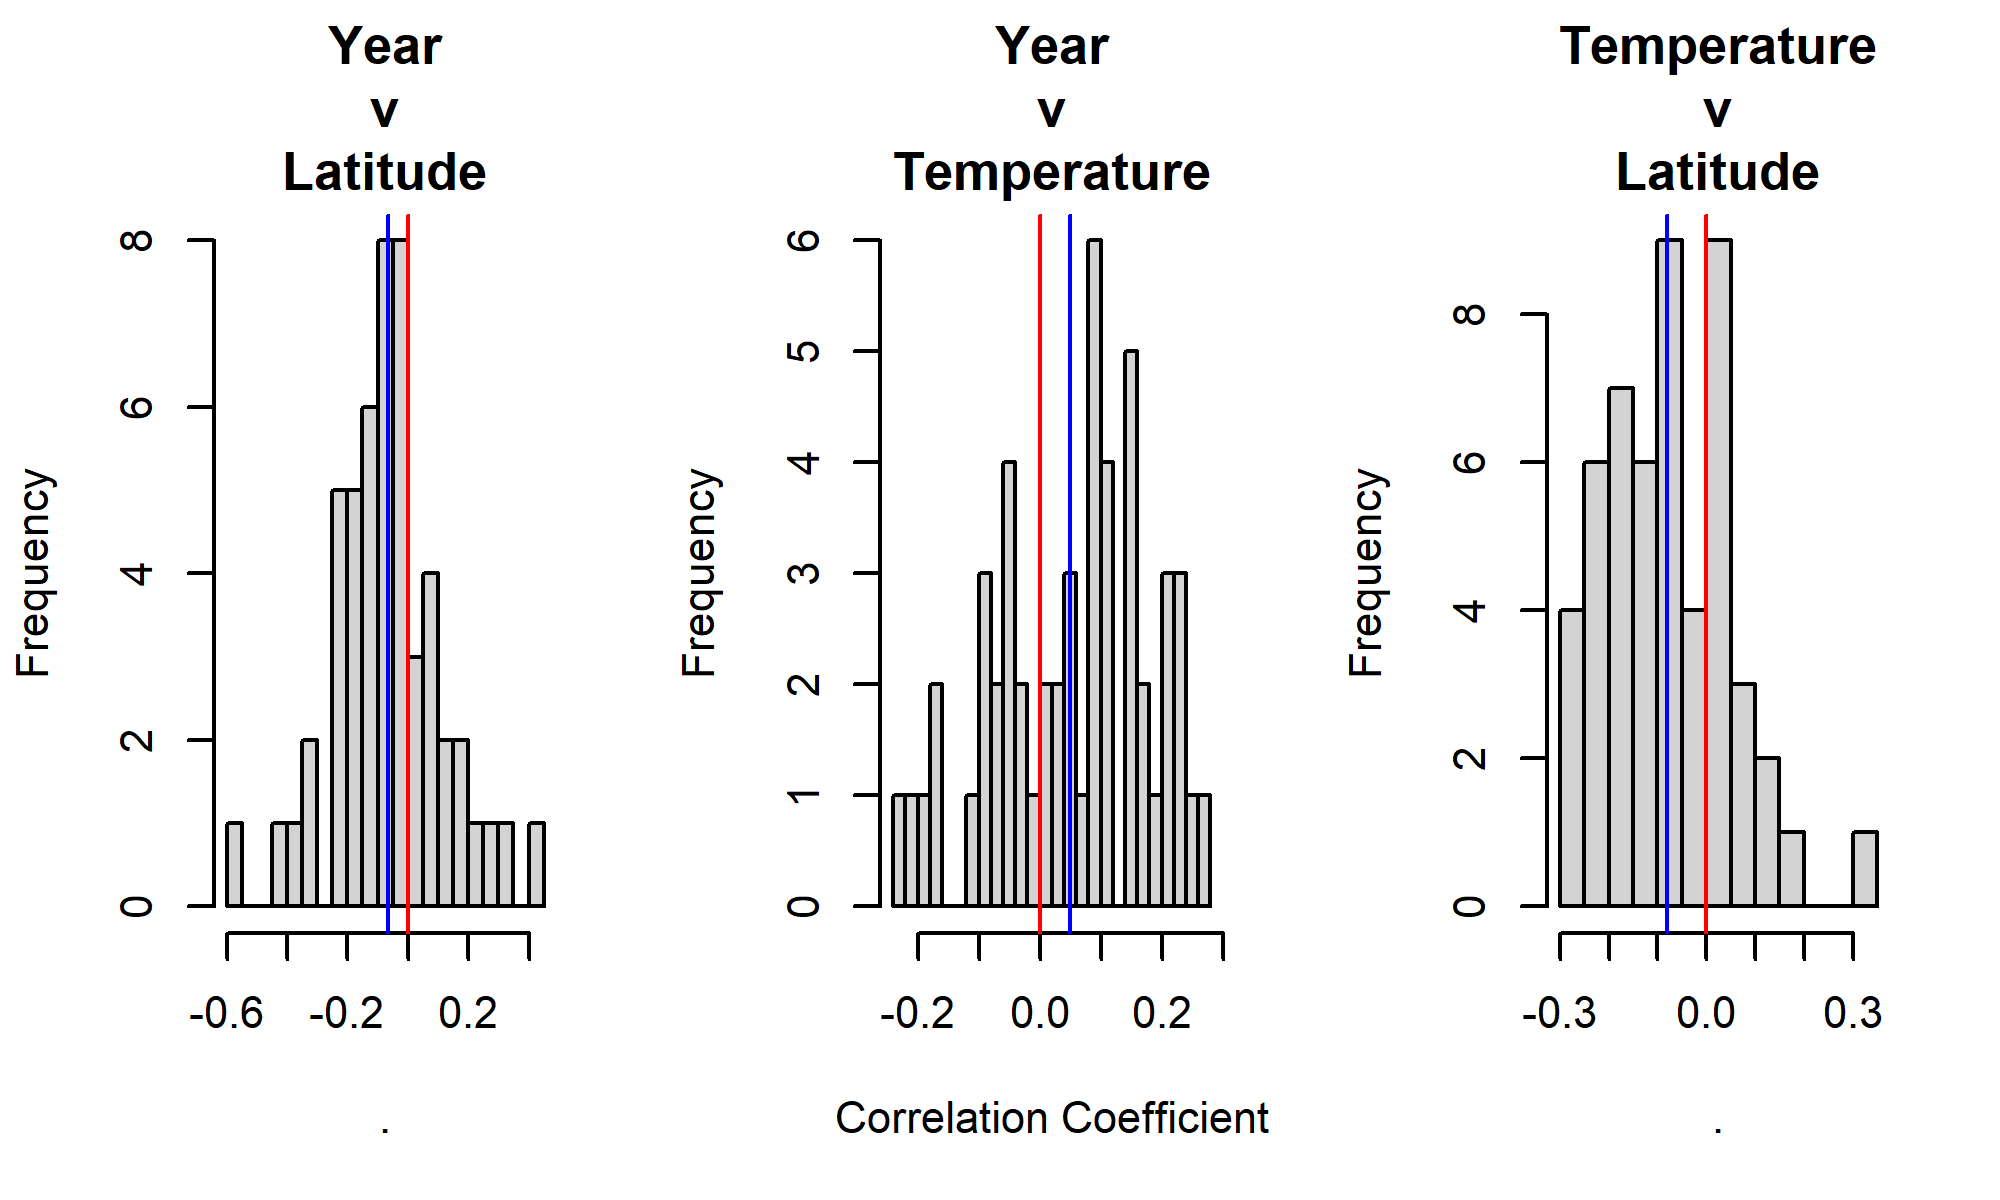
\includegraphics[width=\linewidth]{../figs/SI_corr_inTempLatYear.png}
    \caption{
        \textbf{Distribution of within species-level correlations between key predictors in the records in the NHM dataset.} Red line shows 0, blue line shows median. There is no consistent geographic trend through time. Temperature tended to be positively correlated with year, but the trend is very noisy. Likewise, there is an overall negative correlation between temeprature and latitude, but is neither strong or consistent. 
    }
\end{figure}



\begin{figure}[H]
    \centering
    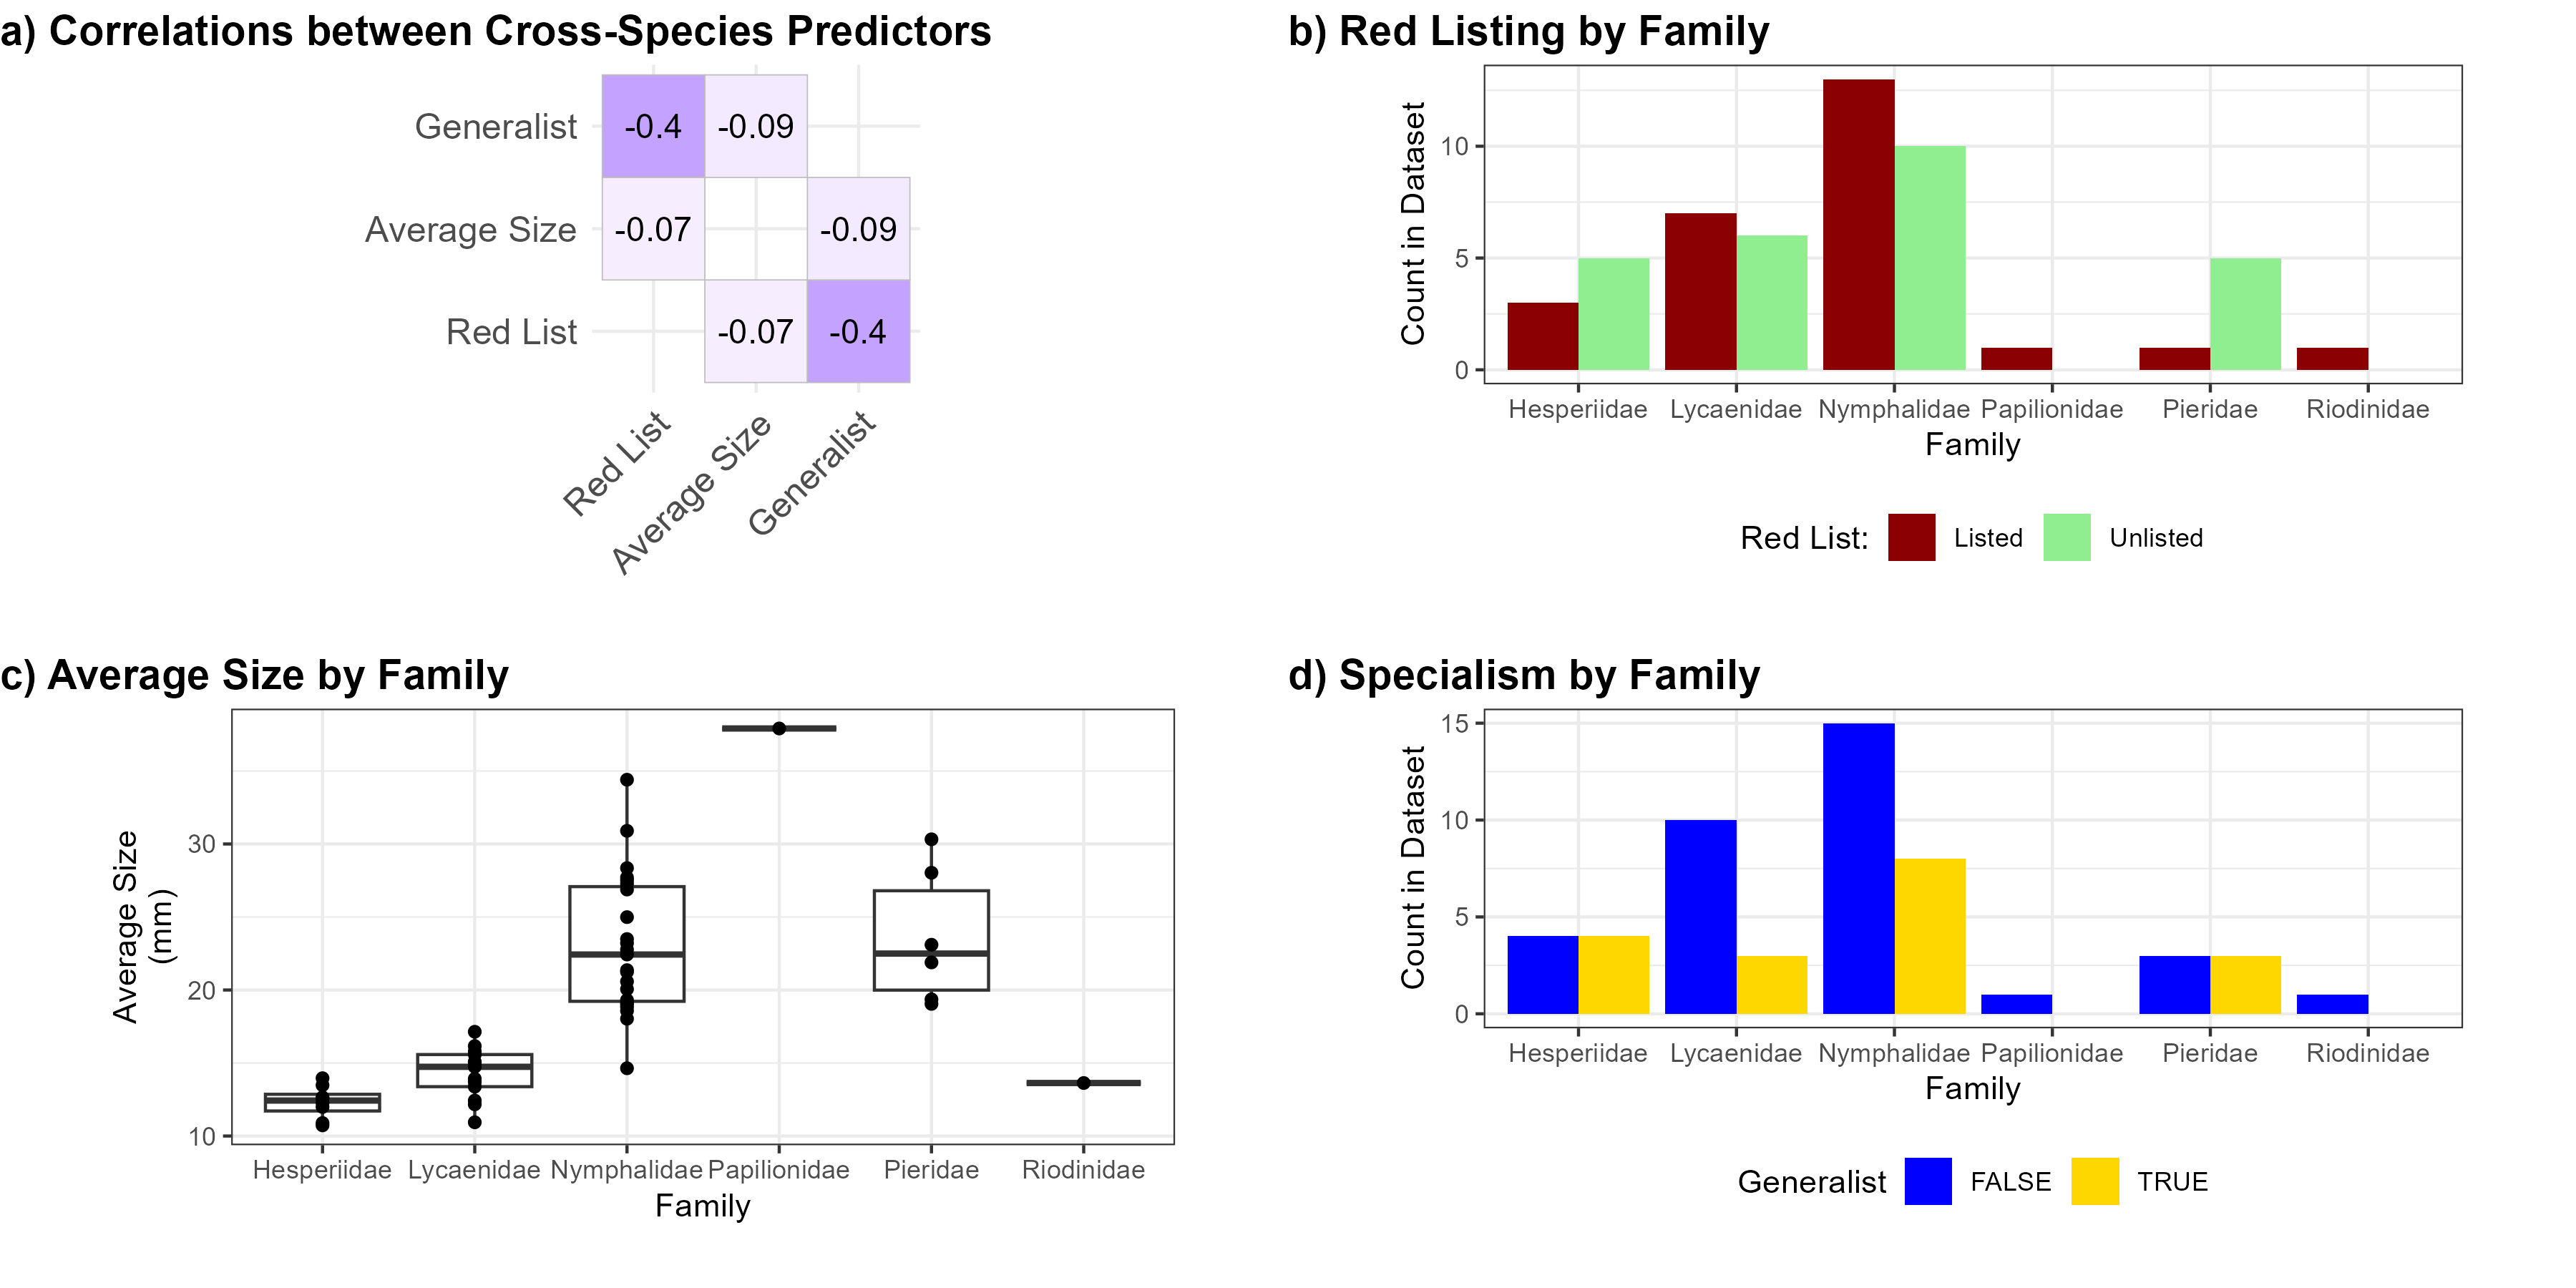
\includegraphics[width=\linewidth]{../figs/SI_correlation_in_predictors.png}
    \caption{
        \textbf{Associations between cross-species predictors.}
        (A) Correlations among the three principal predictors.
        (B) - (D) Relationships between taxonomic family and other species-level predictors.
        Families vary substantially in average size, but are otherwise approximately evenly distributed across predictor space.
    }
\end{figure}

\begin{figure}[H]
    \centering
    \includegraphics[width=\linewidth]{../figs/Corr_sample_size_trends_NHM_Spatial.png}
    \caption{
        \textbf{ Relationship between sample size, confidence of posterior estimate and identification of species-level trends in the NHM dataset.} Precision of posterior estimates was strongly related to the sample size for each species, but the identification of confident trends was less dependent on sample size. 
    }
\end{figure}

\begin{figure}[H]
    \centering
    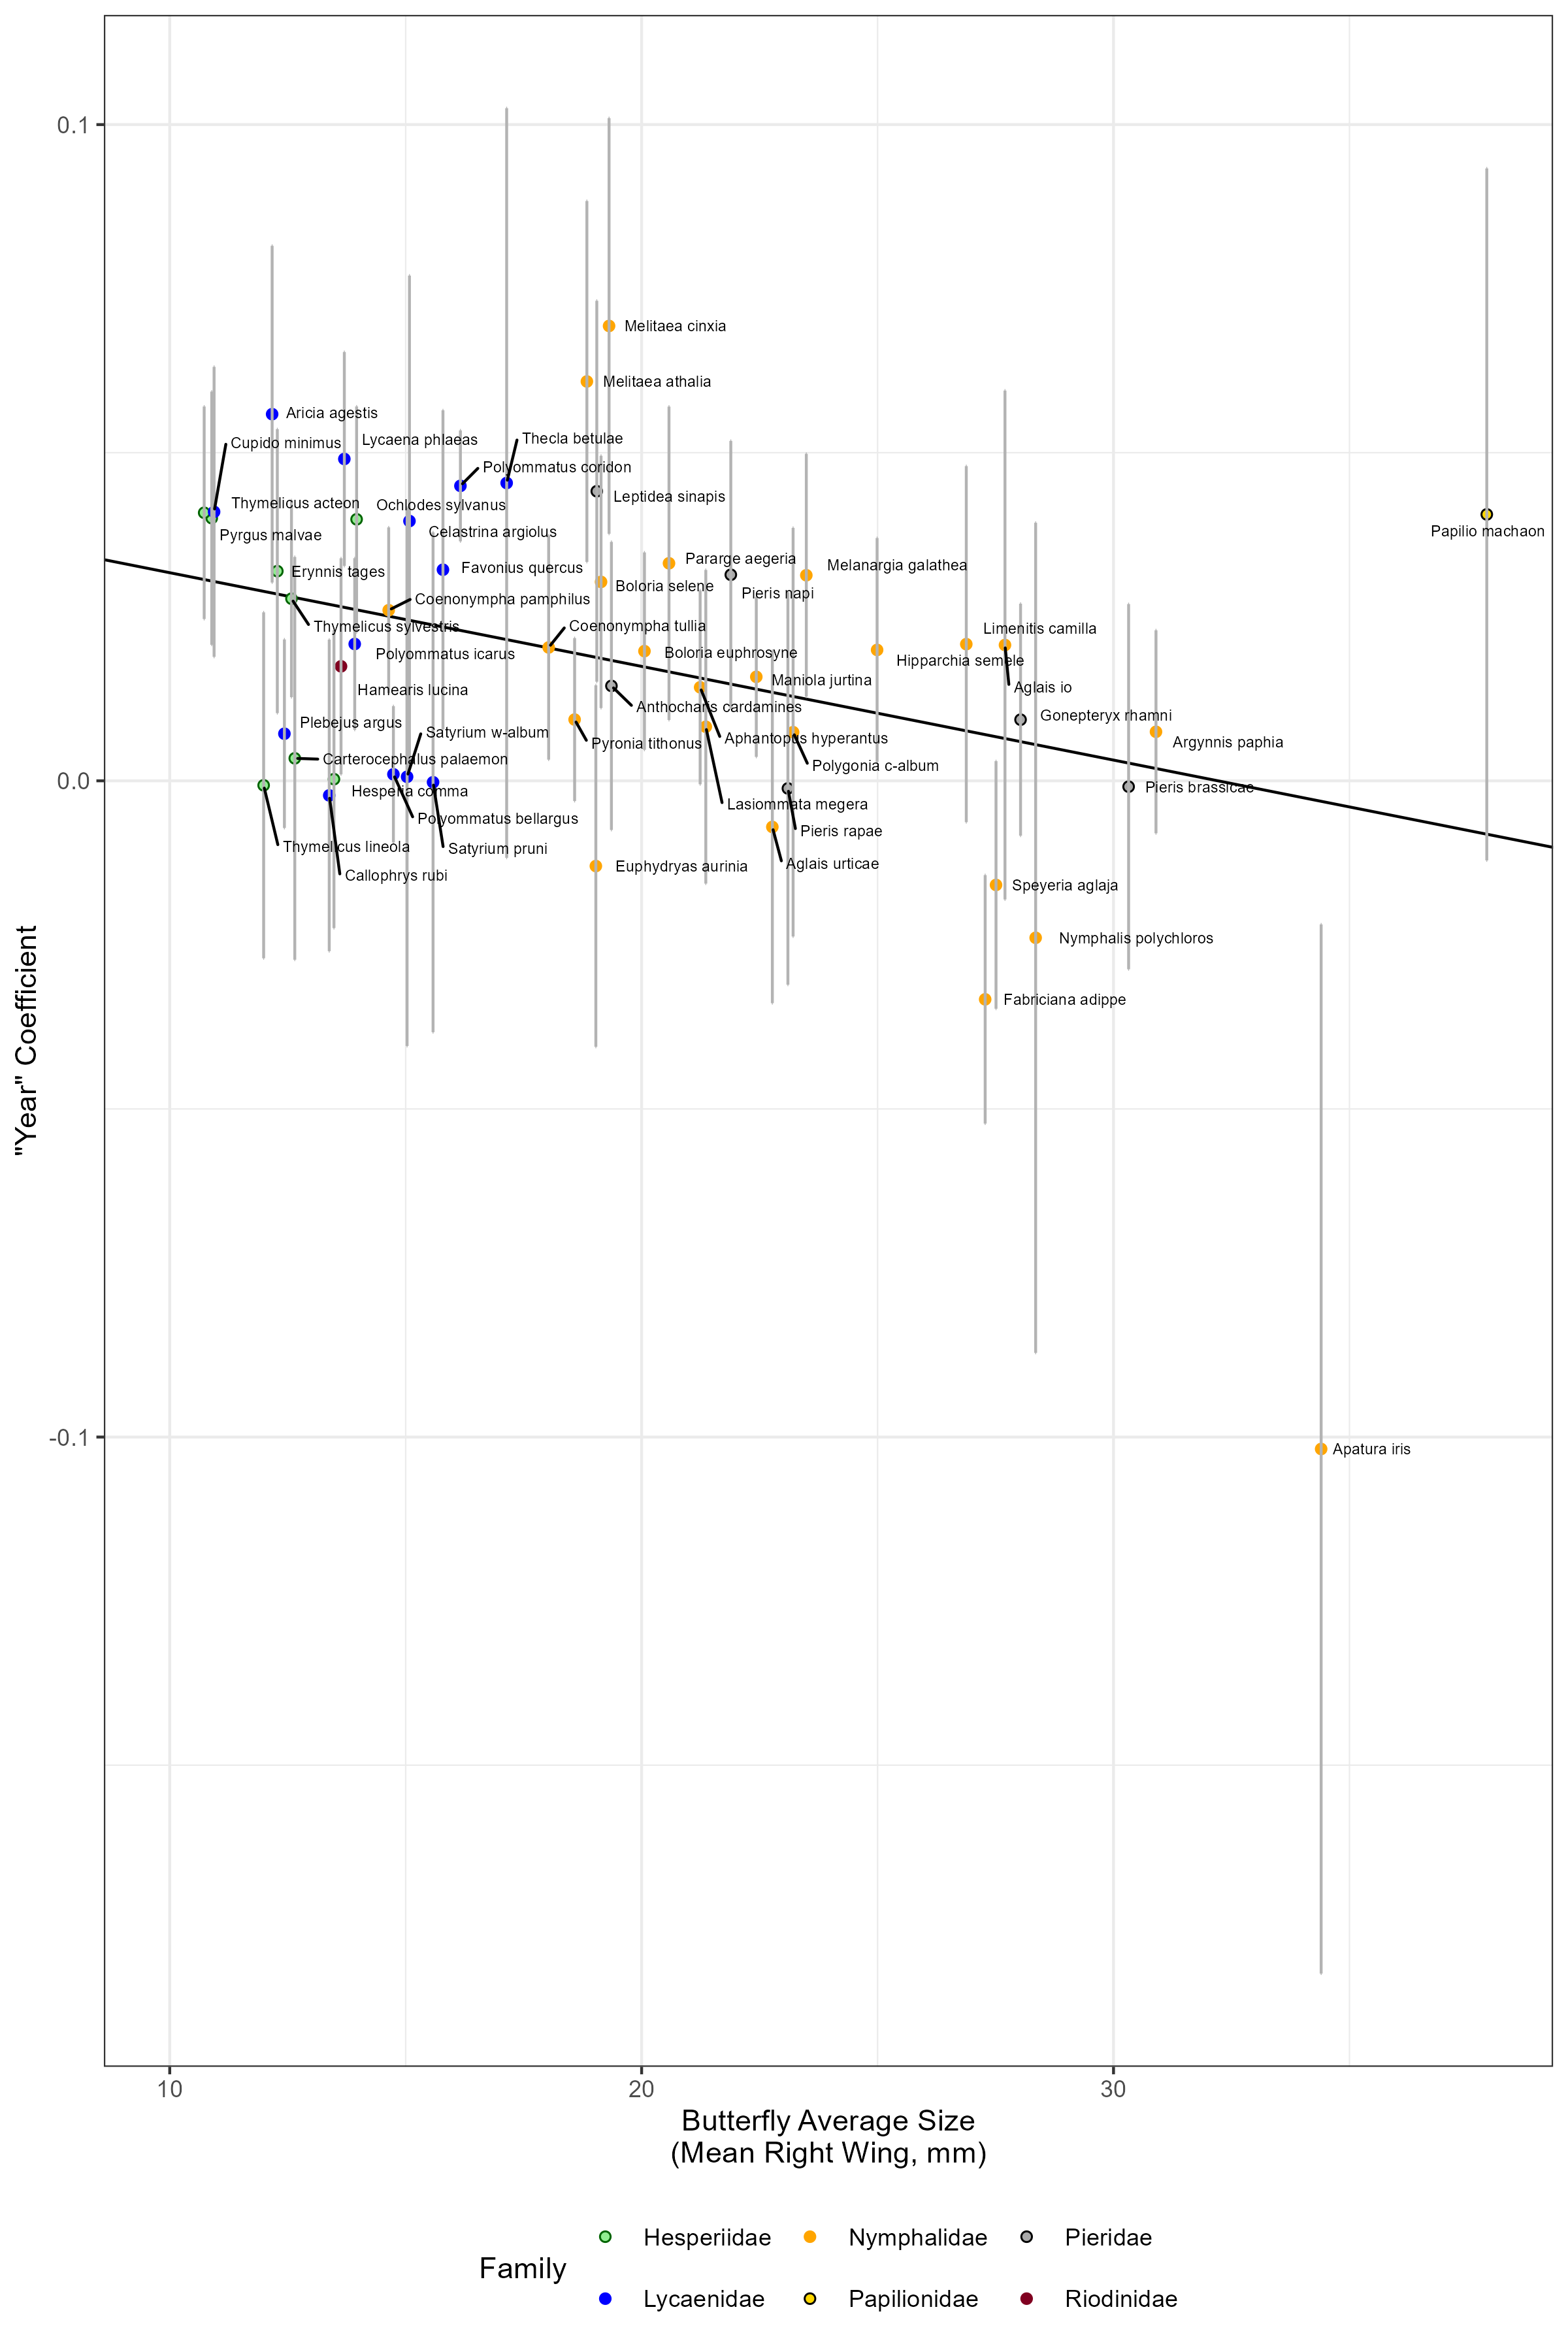
\includegraphics[width=\linewidth]{../figs/PredictorsFigure_4_withlabels_SPATIAL.png}
    \caption{
        \textbf{Main text Figure 4a with species labels and relative uncertaity of each species} Error bars show +/- two standard deviations of the posterior.
    }
\end{figure}


\begin{figure}[H]
    \centering
    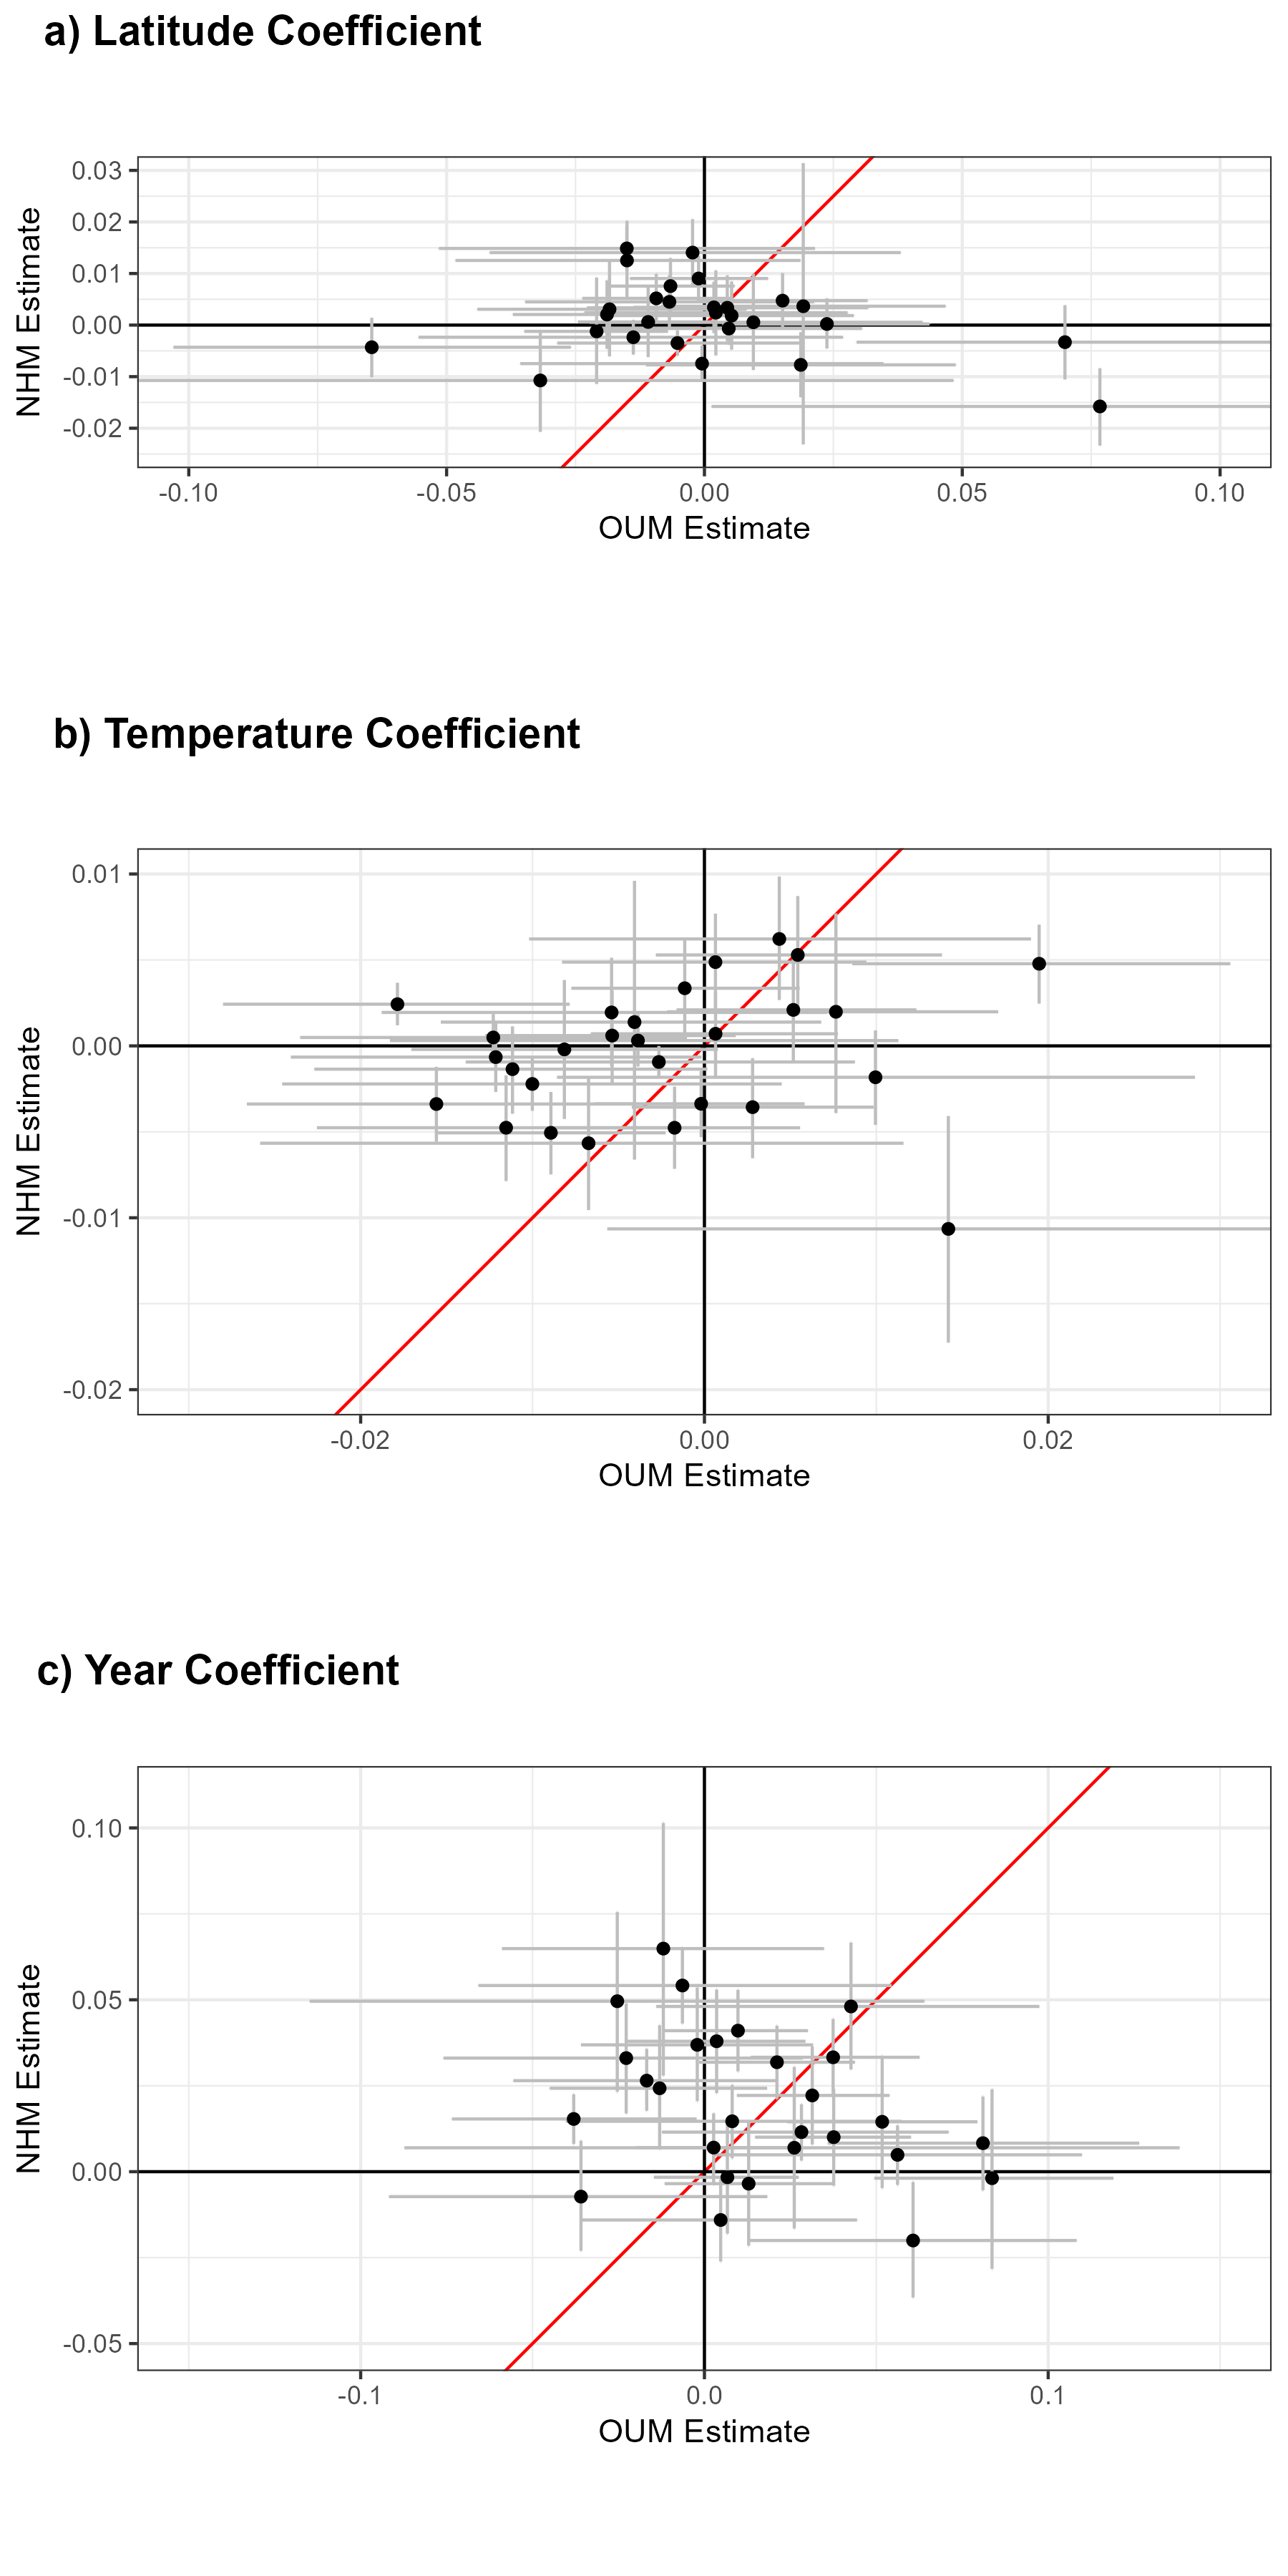
\includegraphics[width=0.6\linewidth]{../figs/compare_coefs_across_datasets.png}
    \caption{
        \textbf{Coefficient Correlations between datasets.} Here, each dot represents a species best-fit coefficent of the record-predictors within the two datasets. Error bars show 90\% posterior confidence interval. Estimates from the smaller dataset were mich more uncertain (note the unequal axis scales). Pearson's correlation of the mean estimates between the datasets was insigificant in each case ( p-values: 0.158, 0.429, 0.0797 respectively (unadjusted for multiple tests)). 
        }
\end{figure}

\begin{figure}[H]
    \centering
    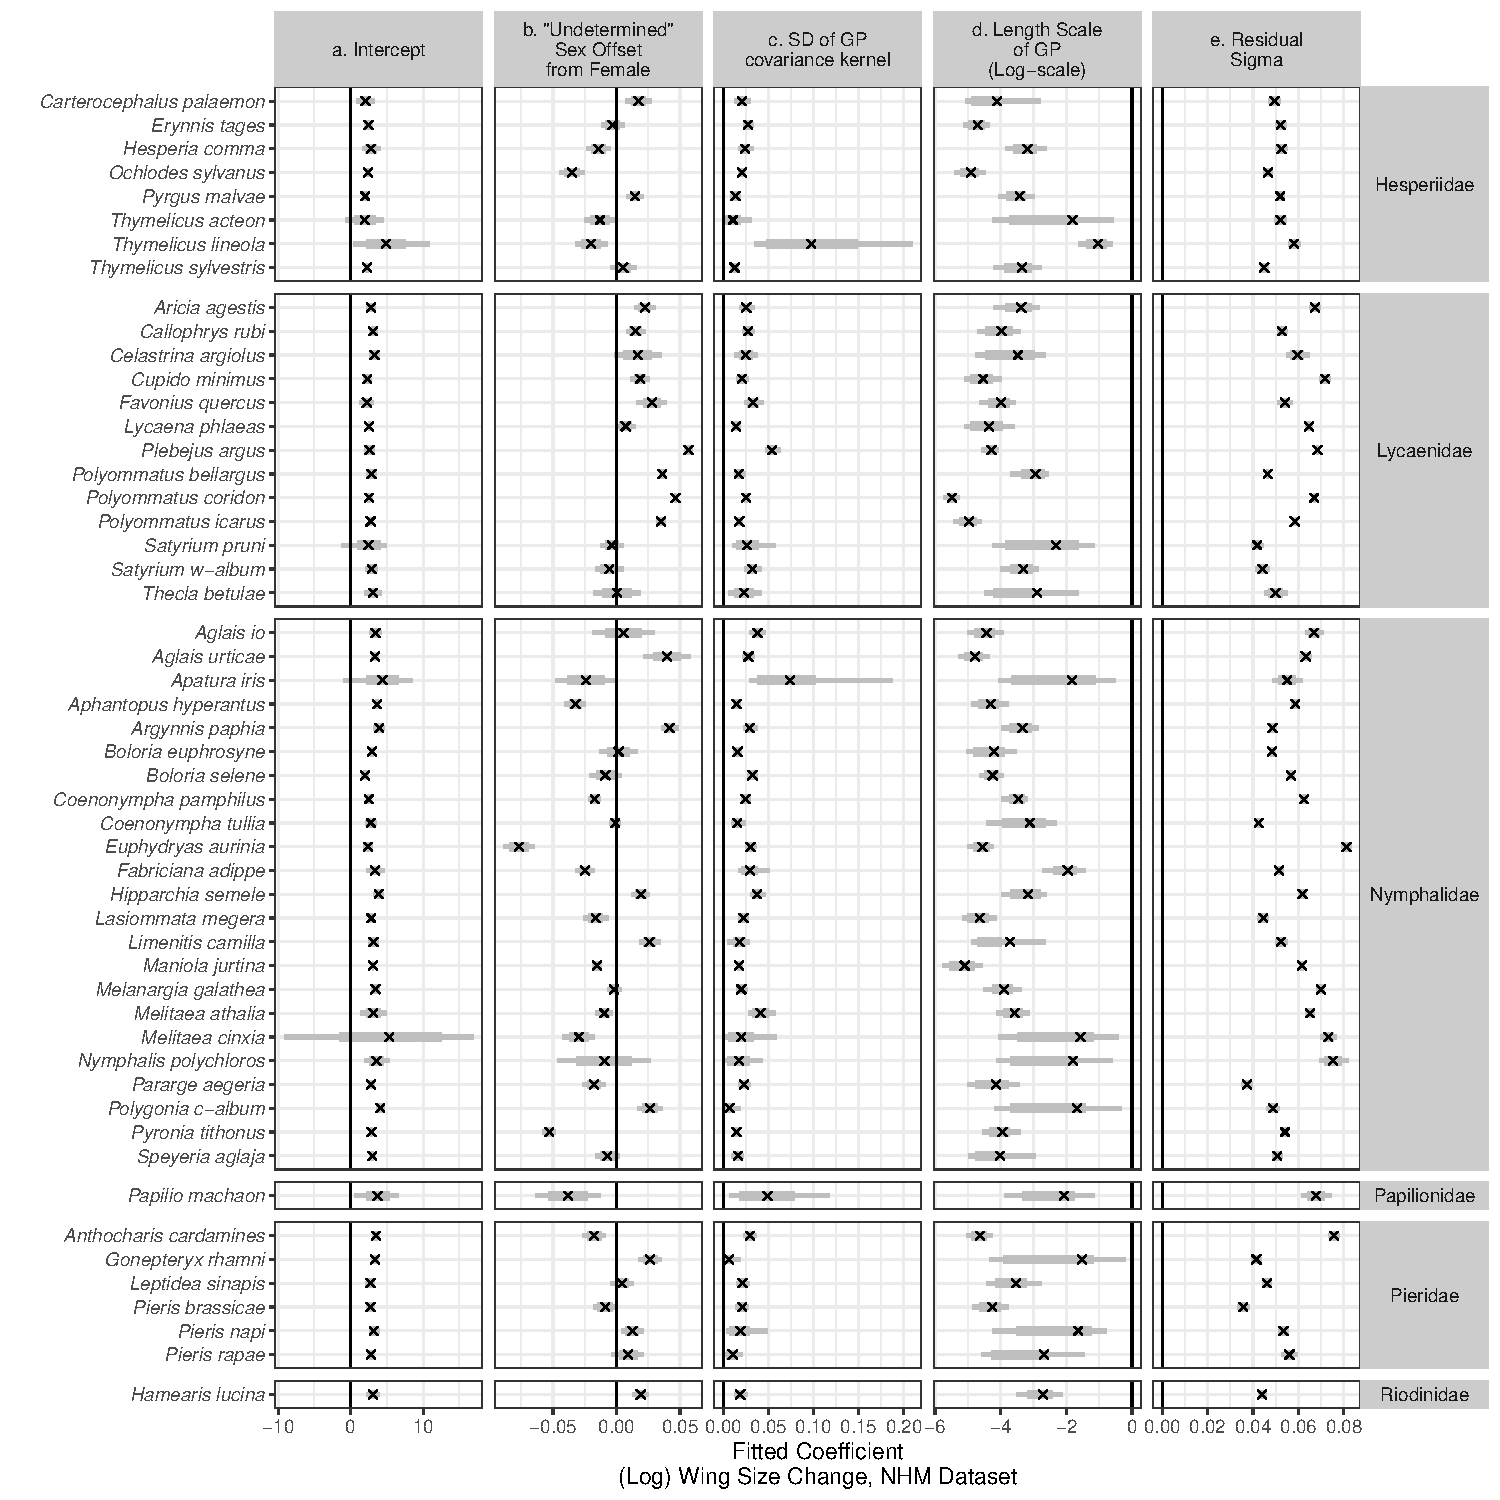
\includegraphics[width=\linewidth]{../figs/SI_NHM_extra_CoefficientPlot.pdf}
    \caption{
        \textbf{Non-focal fitted coefficient posterior distributions from the species level models} Posterior distributions for each species for a) the overall intercept, b) the offset from the female baseline for sex-undetermined specimens. This would include a mixture of males and females, but in variable proportions, c) the standard deviation of the Gaussian process covariance kernel (logged for comparability between species),  d) 	length-scale of the Gaussian process covariance kernel, e) estimated residual variation ($\sigma$). 
        }
\end{figure}

\begin{figure}[H]
    \centering
    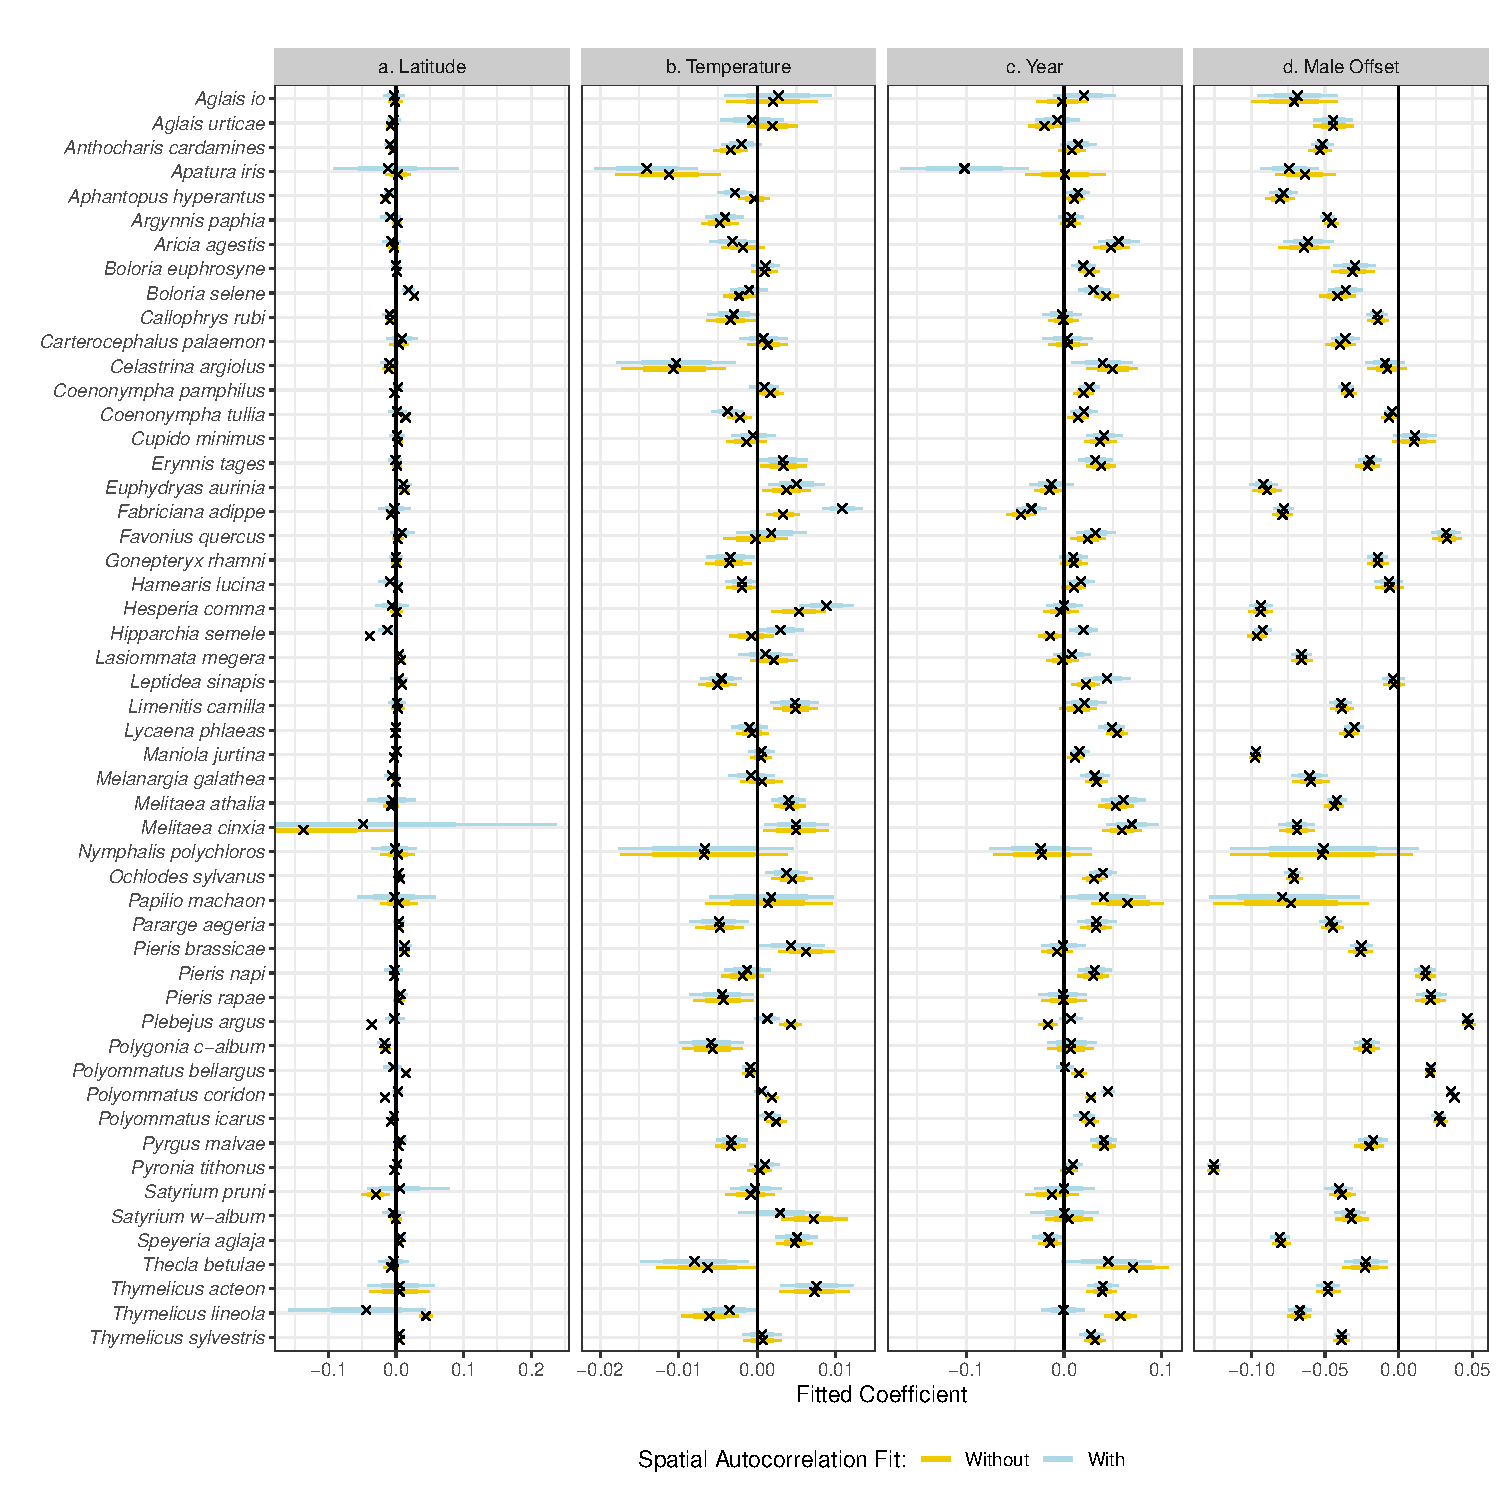
\includegraphics[width=\linewidth]{../figs/Compare_Spatial_NonSpatial.pdf}
    \caption{
        \textbf{Impact on fitted coefficient posteriors for NHM dataset of also including spatial autocorrelation term thorough a Gaussian point process.} Lines show 90\% and 66\% intervals. For almost all species, even though the GPP was informative for the purposes of prediction, the coefficents to be carried forward to the cross-species models are highly comparable. Cross-species regression analyses gave very similar results without the GPP term: effect of Size on Year coefficent (i.e. result presented in main text Fig 4a): -0.001435381 (95\% interval: -0.002451985 to -4.021077e-04) and  effect of Red Listing  on Temperature coefficient (i.e. result presented in main text Fig 4b):  -0.00217 (95\% interval:-0.0041 to -0.00018).}
\end{figure}




\begin{figure}[H]
    \centering
    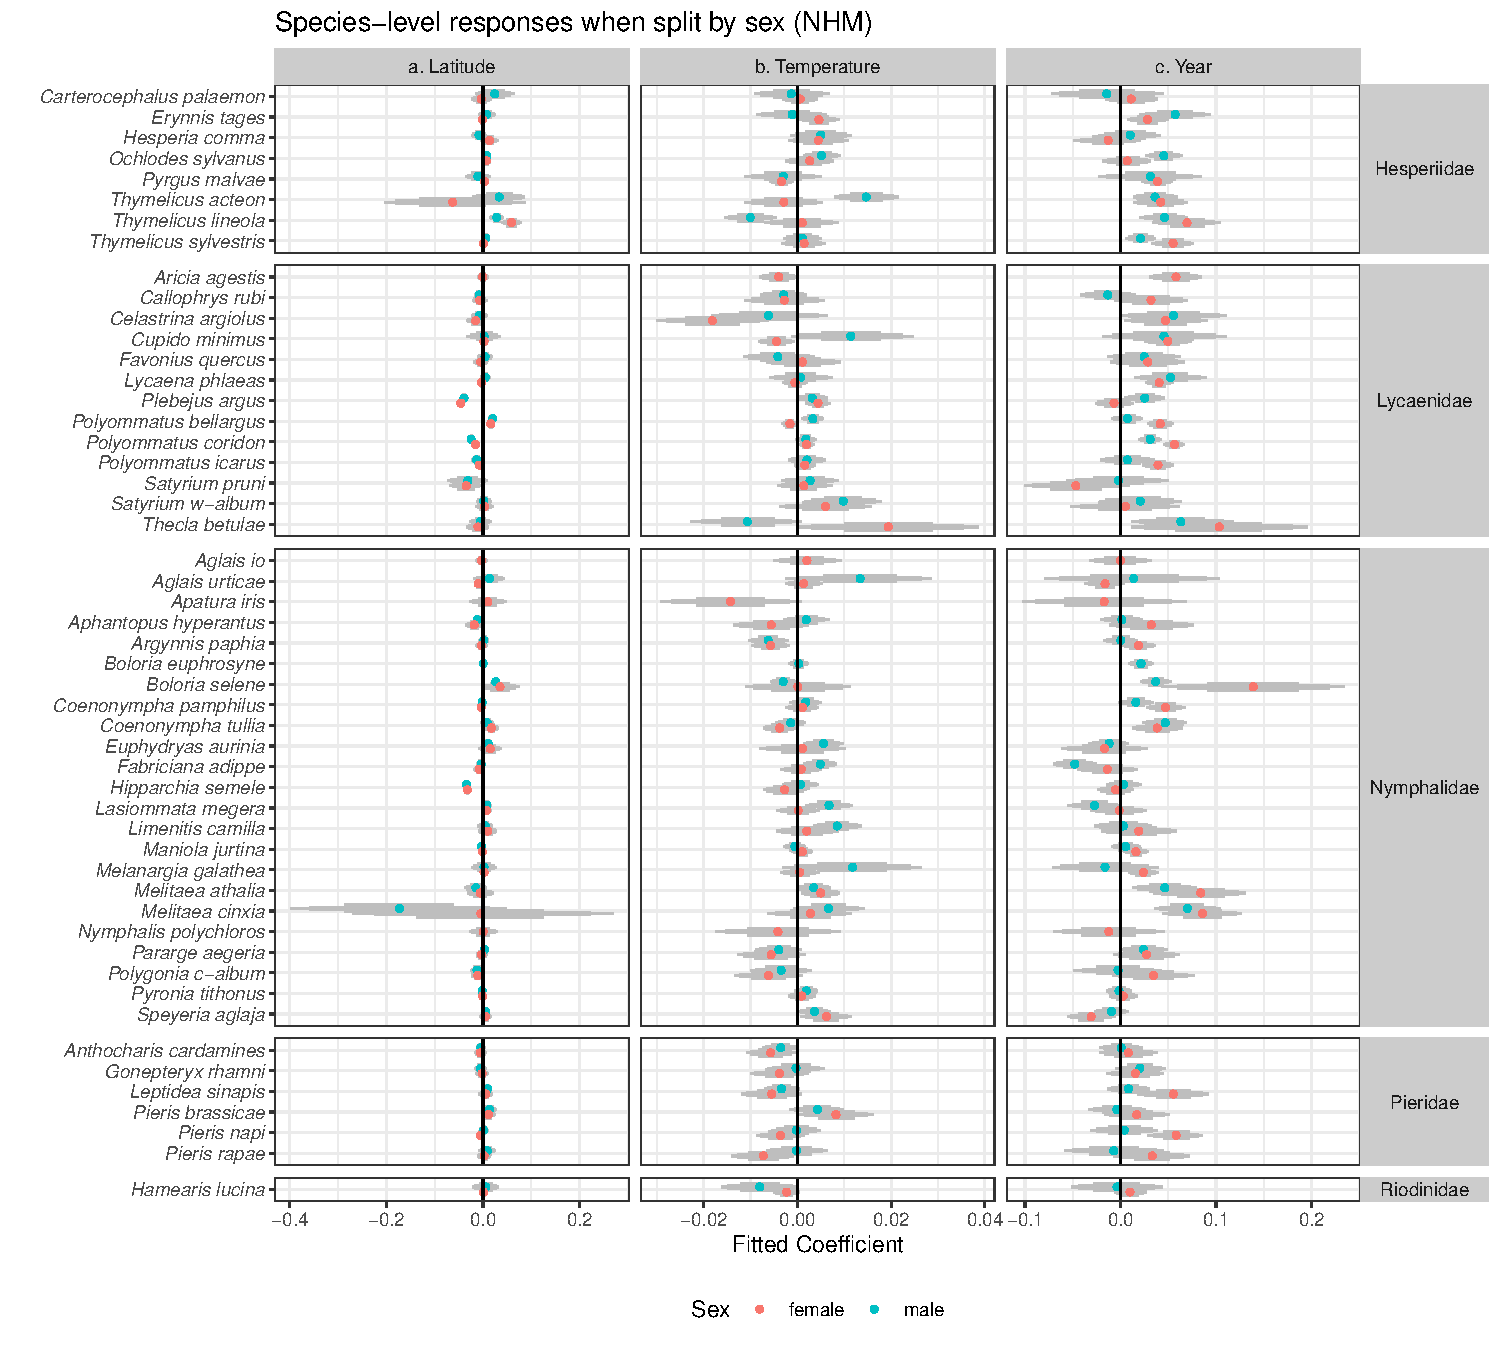
\includegraphics[width=\linewidth]{../figs/NHM_Monthly_MainSpResults_SplitSexSp.pdf}
    \caption{
        \textbf{Investigation of sex-specific responses to predictor variables} Species-level regressions models were refit (without the spatial term) for each sex separately to investigate possible sex-specific responses to the predictors. Note that the degree and balance of sex-determination varied considerably between species due to ease of identification - for five species (\textit{Aglais io}, \textit{Apatura iris}, \textit{Aricia agestis}, 
\textit{Nymphalis polychloros}, \textit{Boloria euphrosyne}) these splits were not possible. Grey lines show 95\%, 90\% and 66\% intervals. Direct comparison of posteriors identified that in 17/138 comparisons the central 95\% of the posterior difference did not overlap zero.}
\end{figure}


\begin{figure}[H]
    \centering
    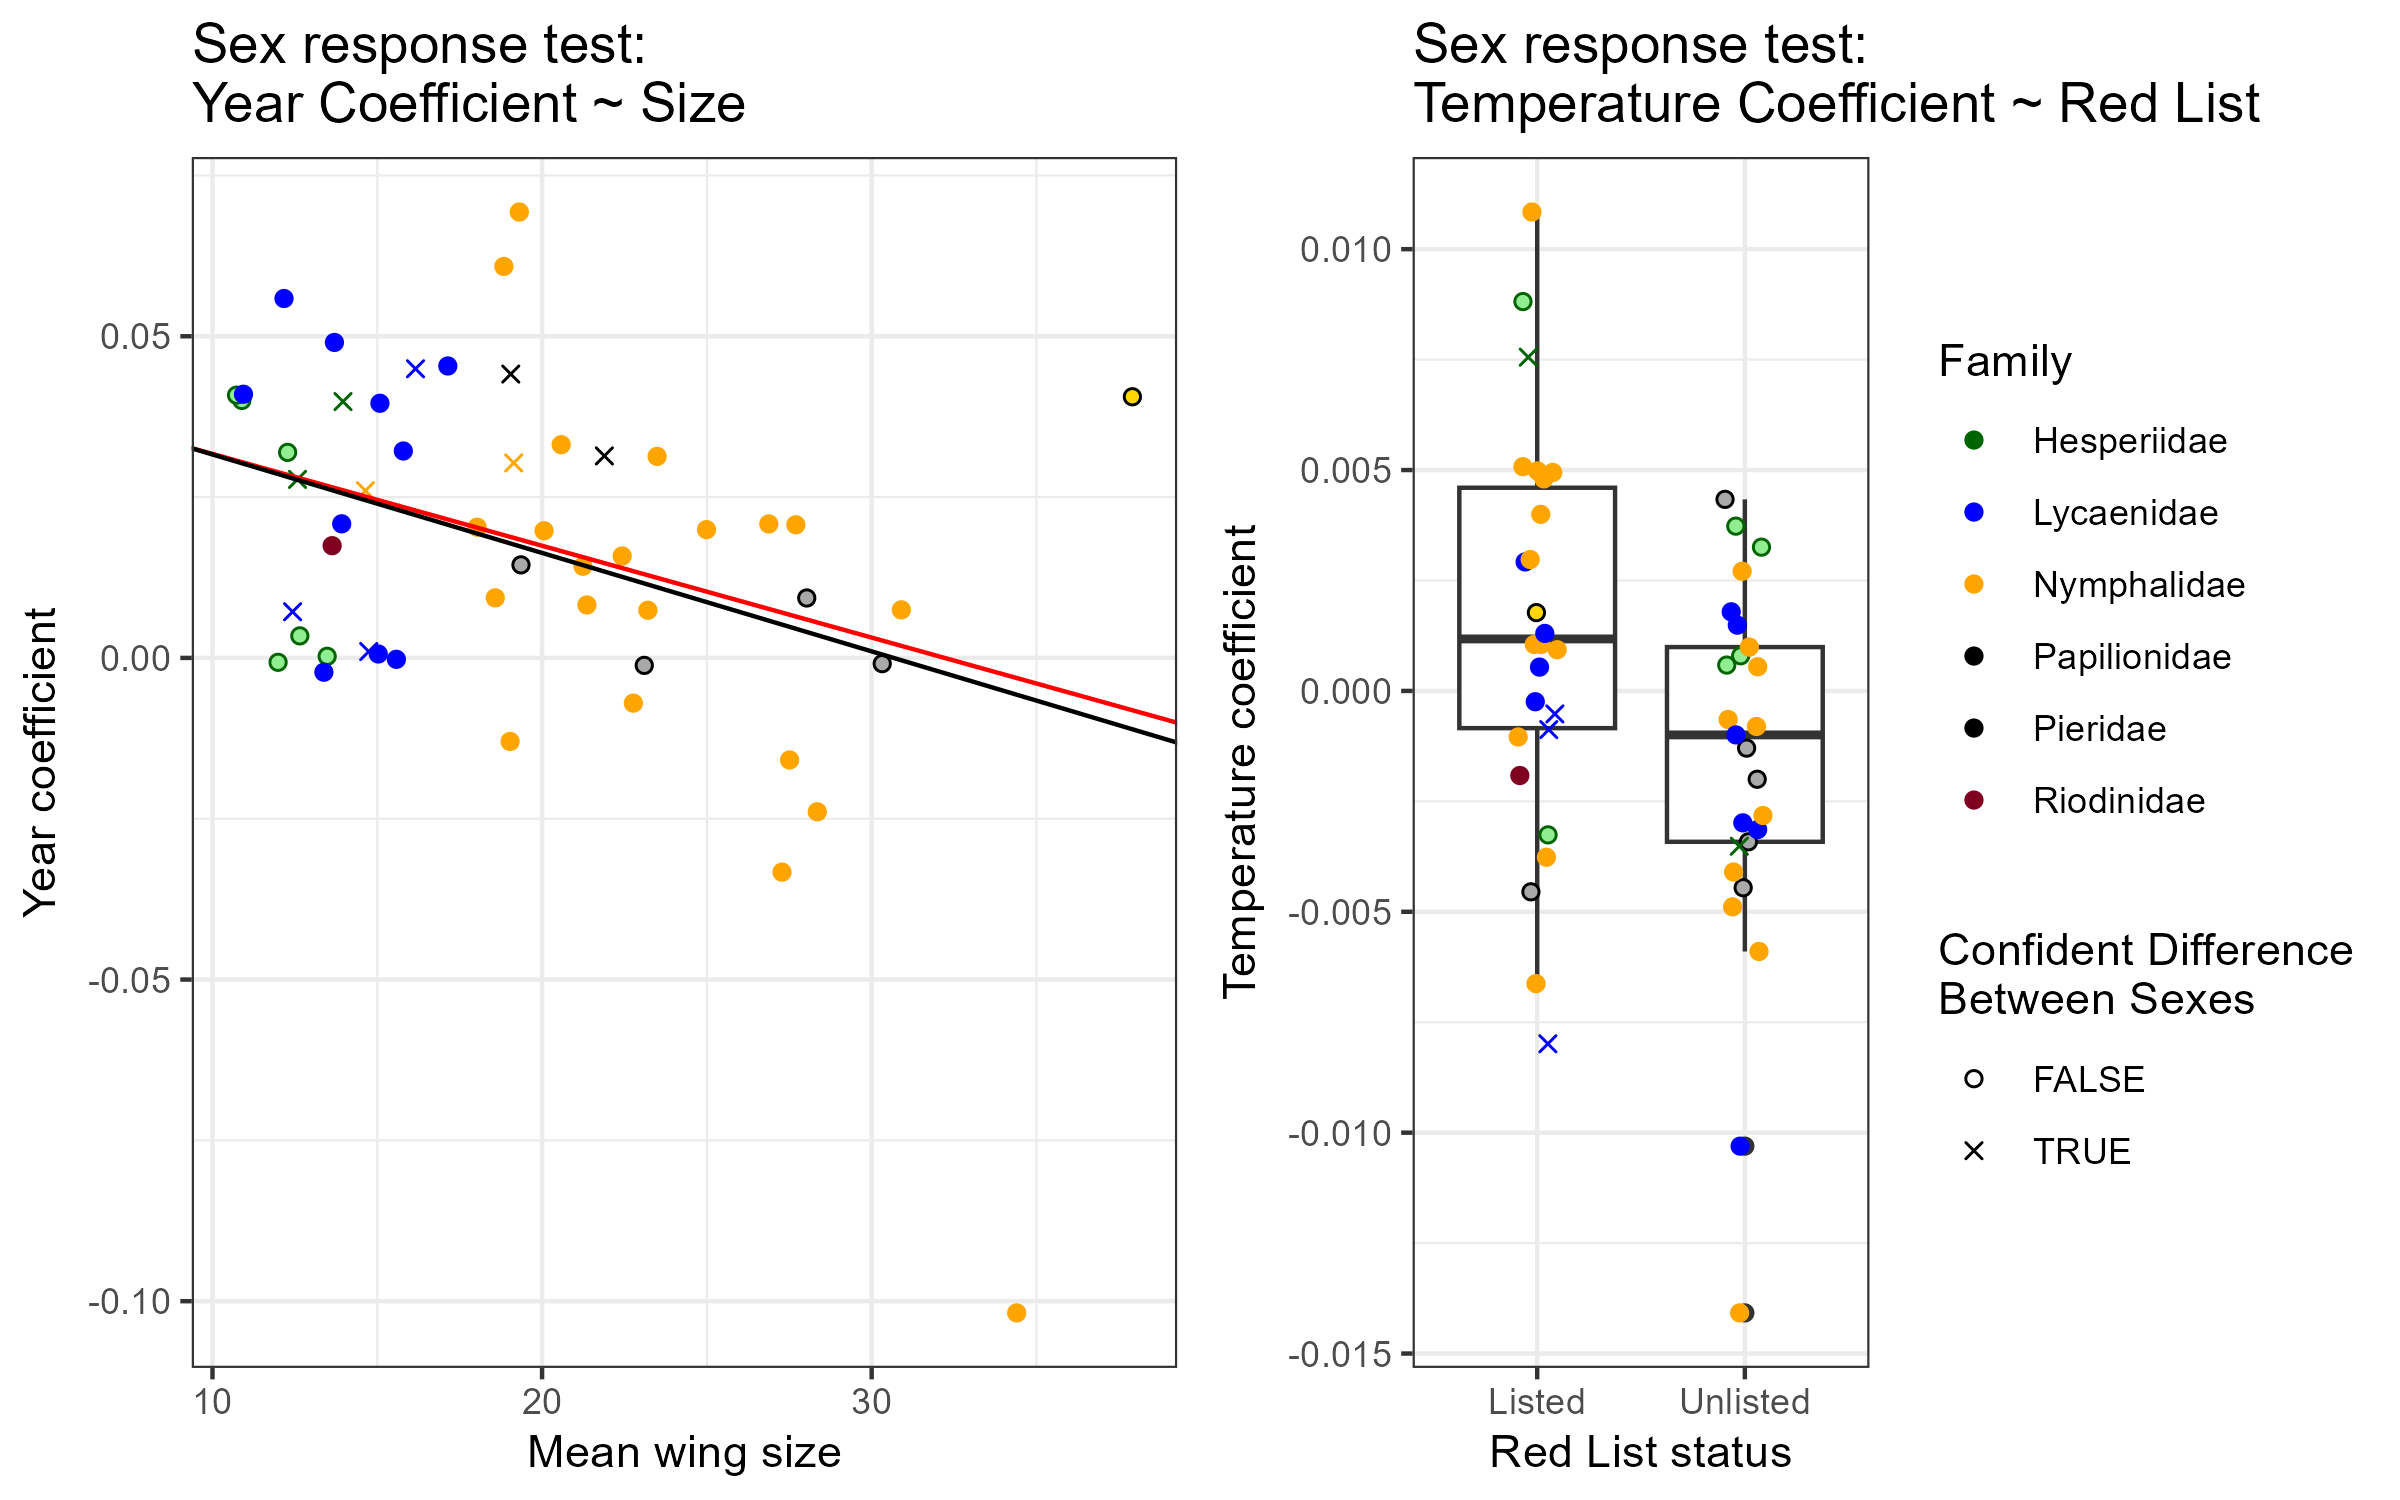
\includegraphics[width=\linewidth]{../figs/Fig4_wosplitsex}
    \caption{
        \textbf{Repeat of Figure 4, excluding species coefficients where potential sex-specific response to predictors were identified}. a) Year coefficent vs Size. Black line shows central estimate of regression without excluded species (slope:-0.0015, 95\% interval: -0.0025 to -0.00055), red line shows main result with all species. b) Temperature Coefficient vs Red List Status. Boxplots do not include species with apparent sex-differences in responses. Estimated difference between Red listing status: -0.0029 (95\% interval: -0.0051 to  -0.0007).}
\end{figure}


\newpage

\section{Specimen Spatio-temporal Distributions}


\begin{figure}[H]
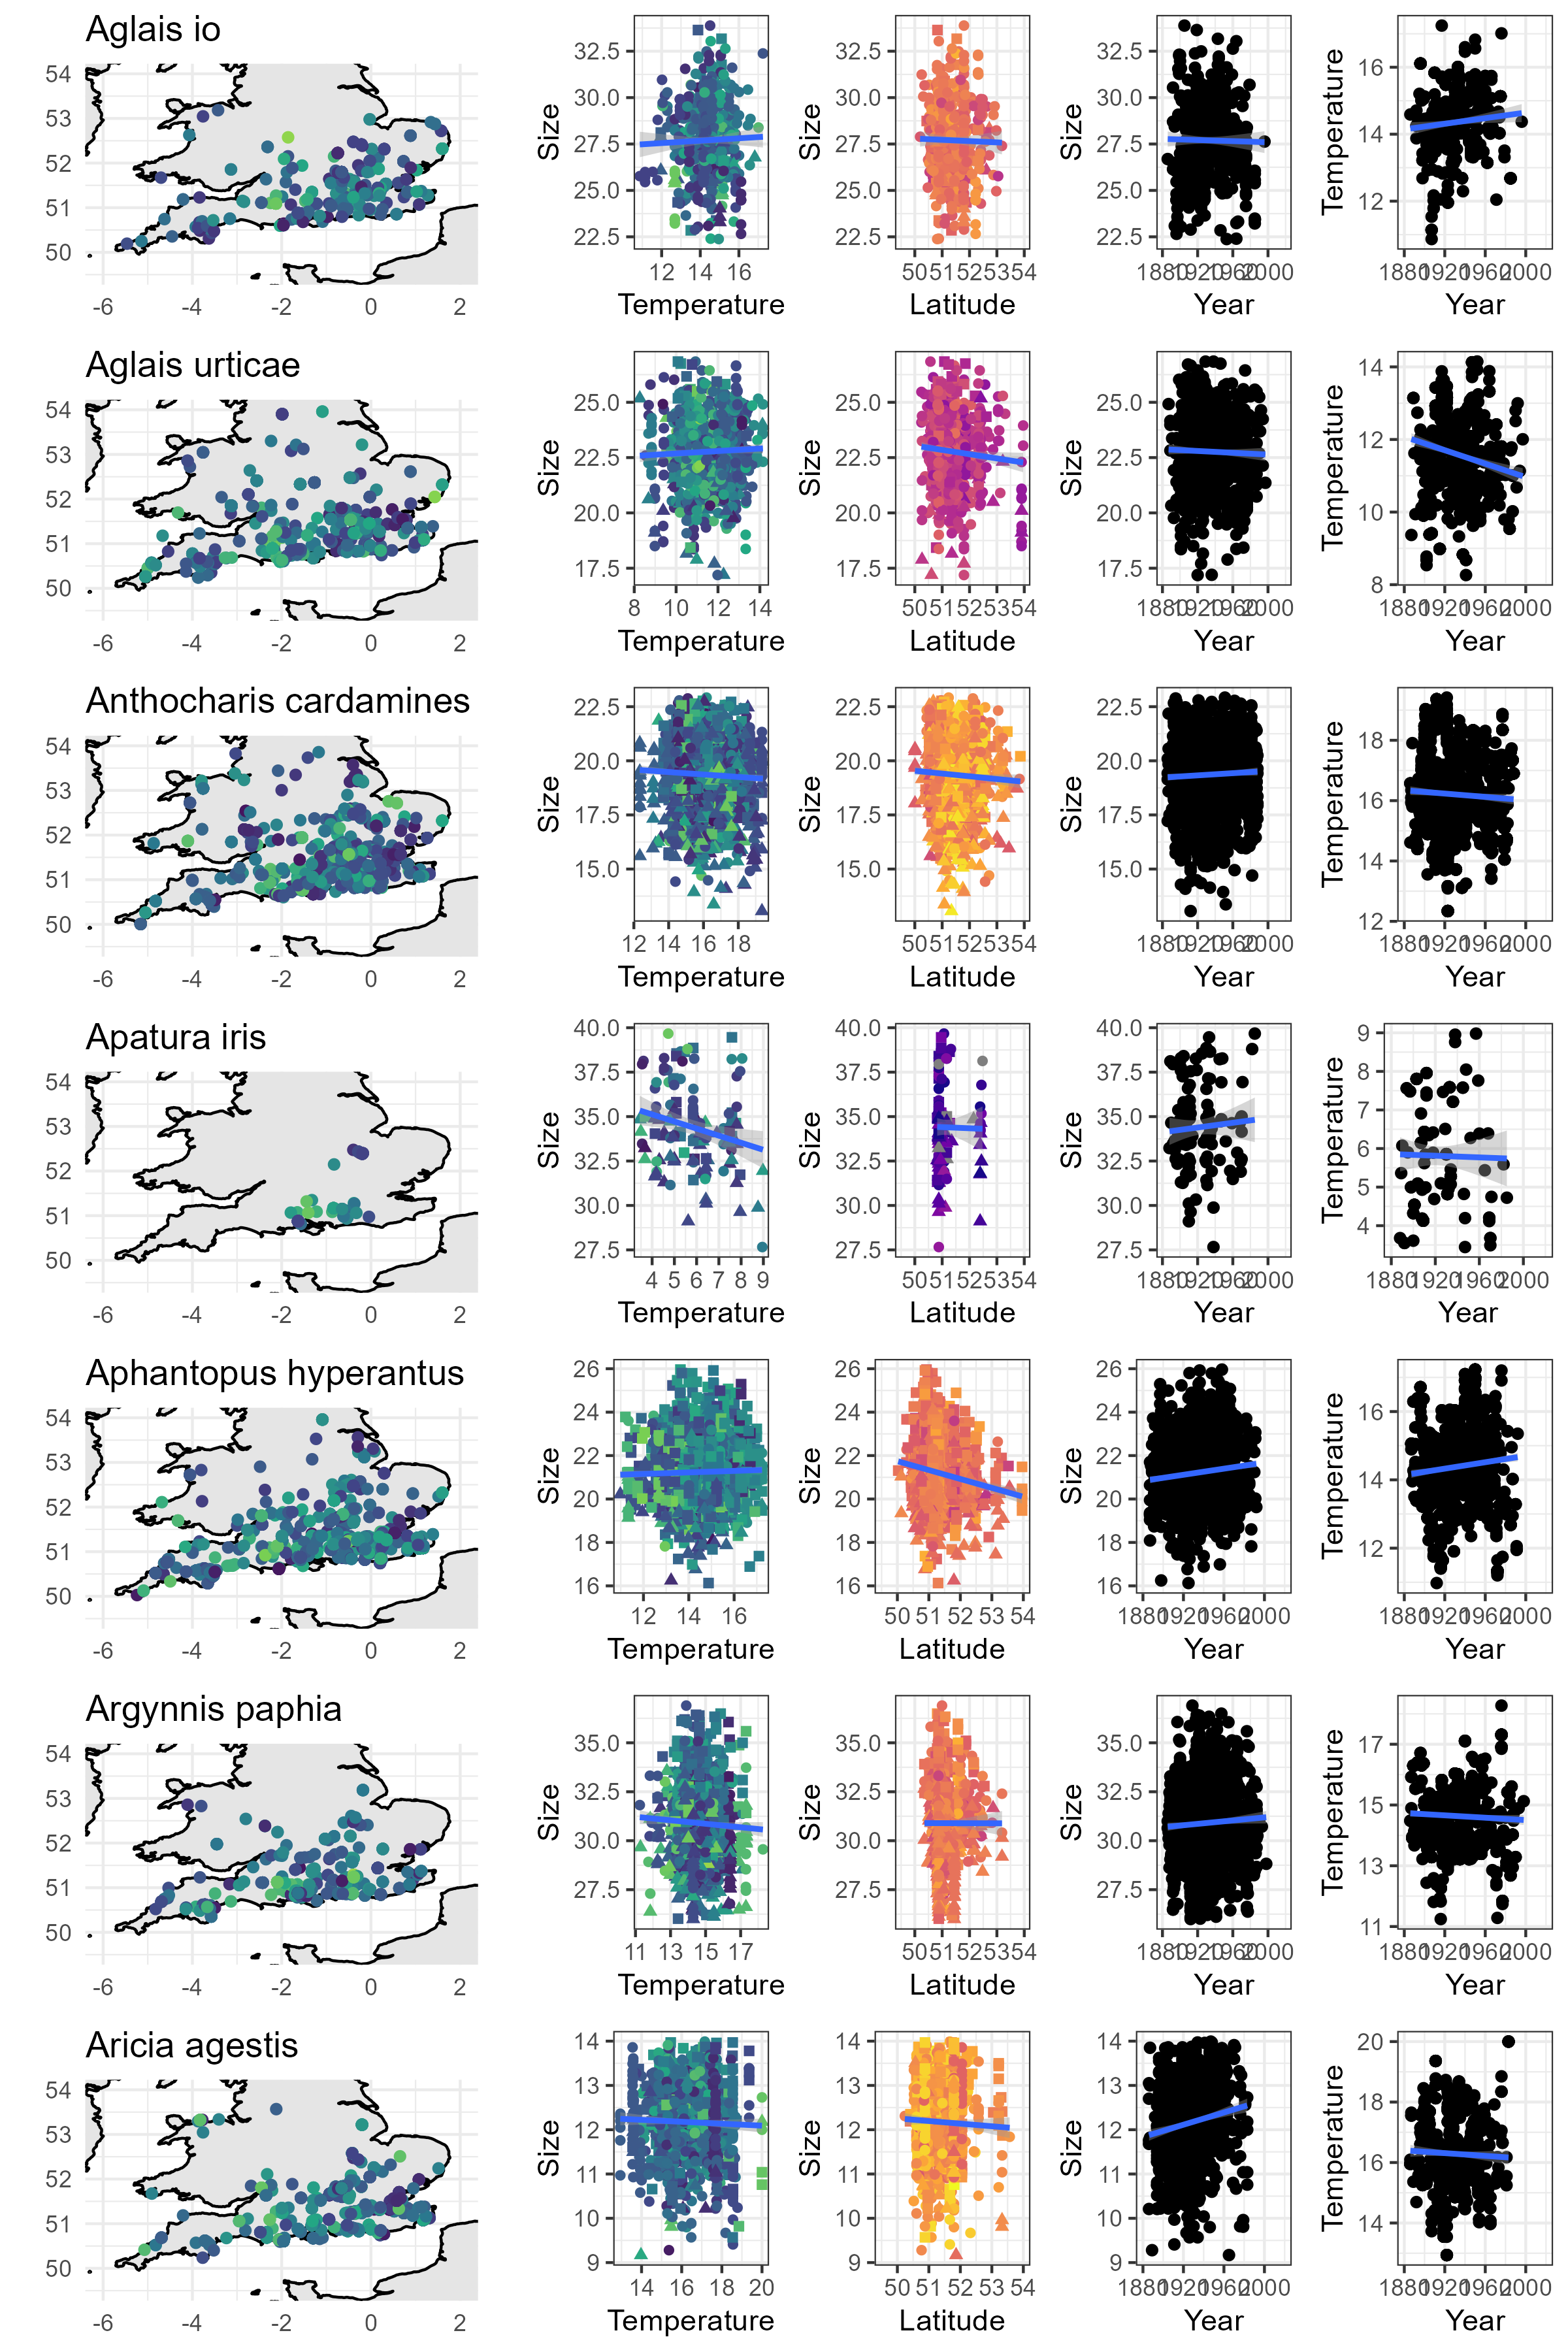
\includegraphics[width=\linewidth]{../figs/SI_NHM_dataspread_1.png}
\end{figure}
\begin{figure}[H]
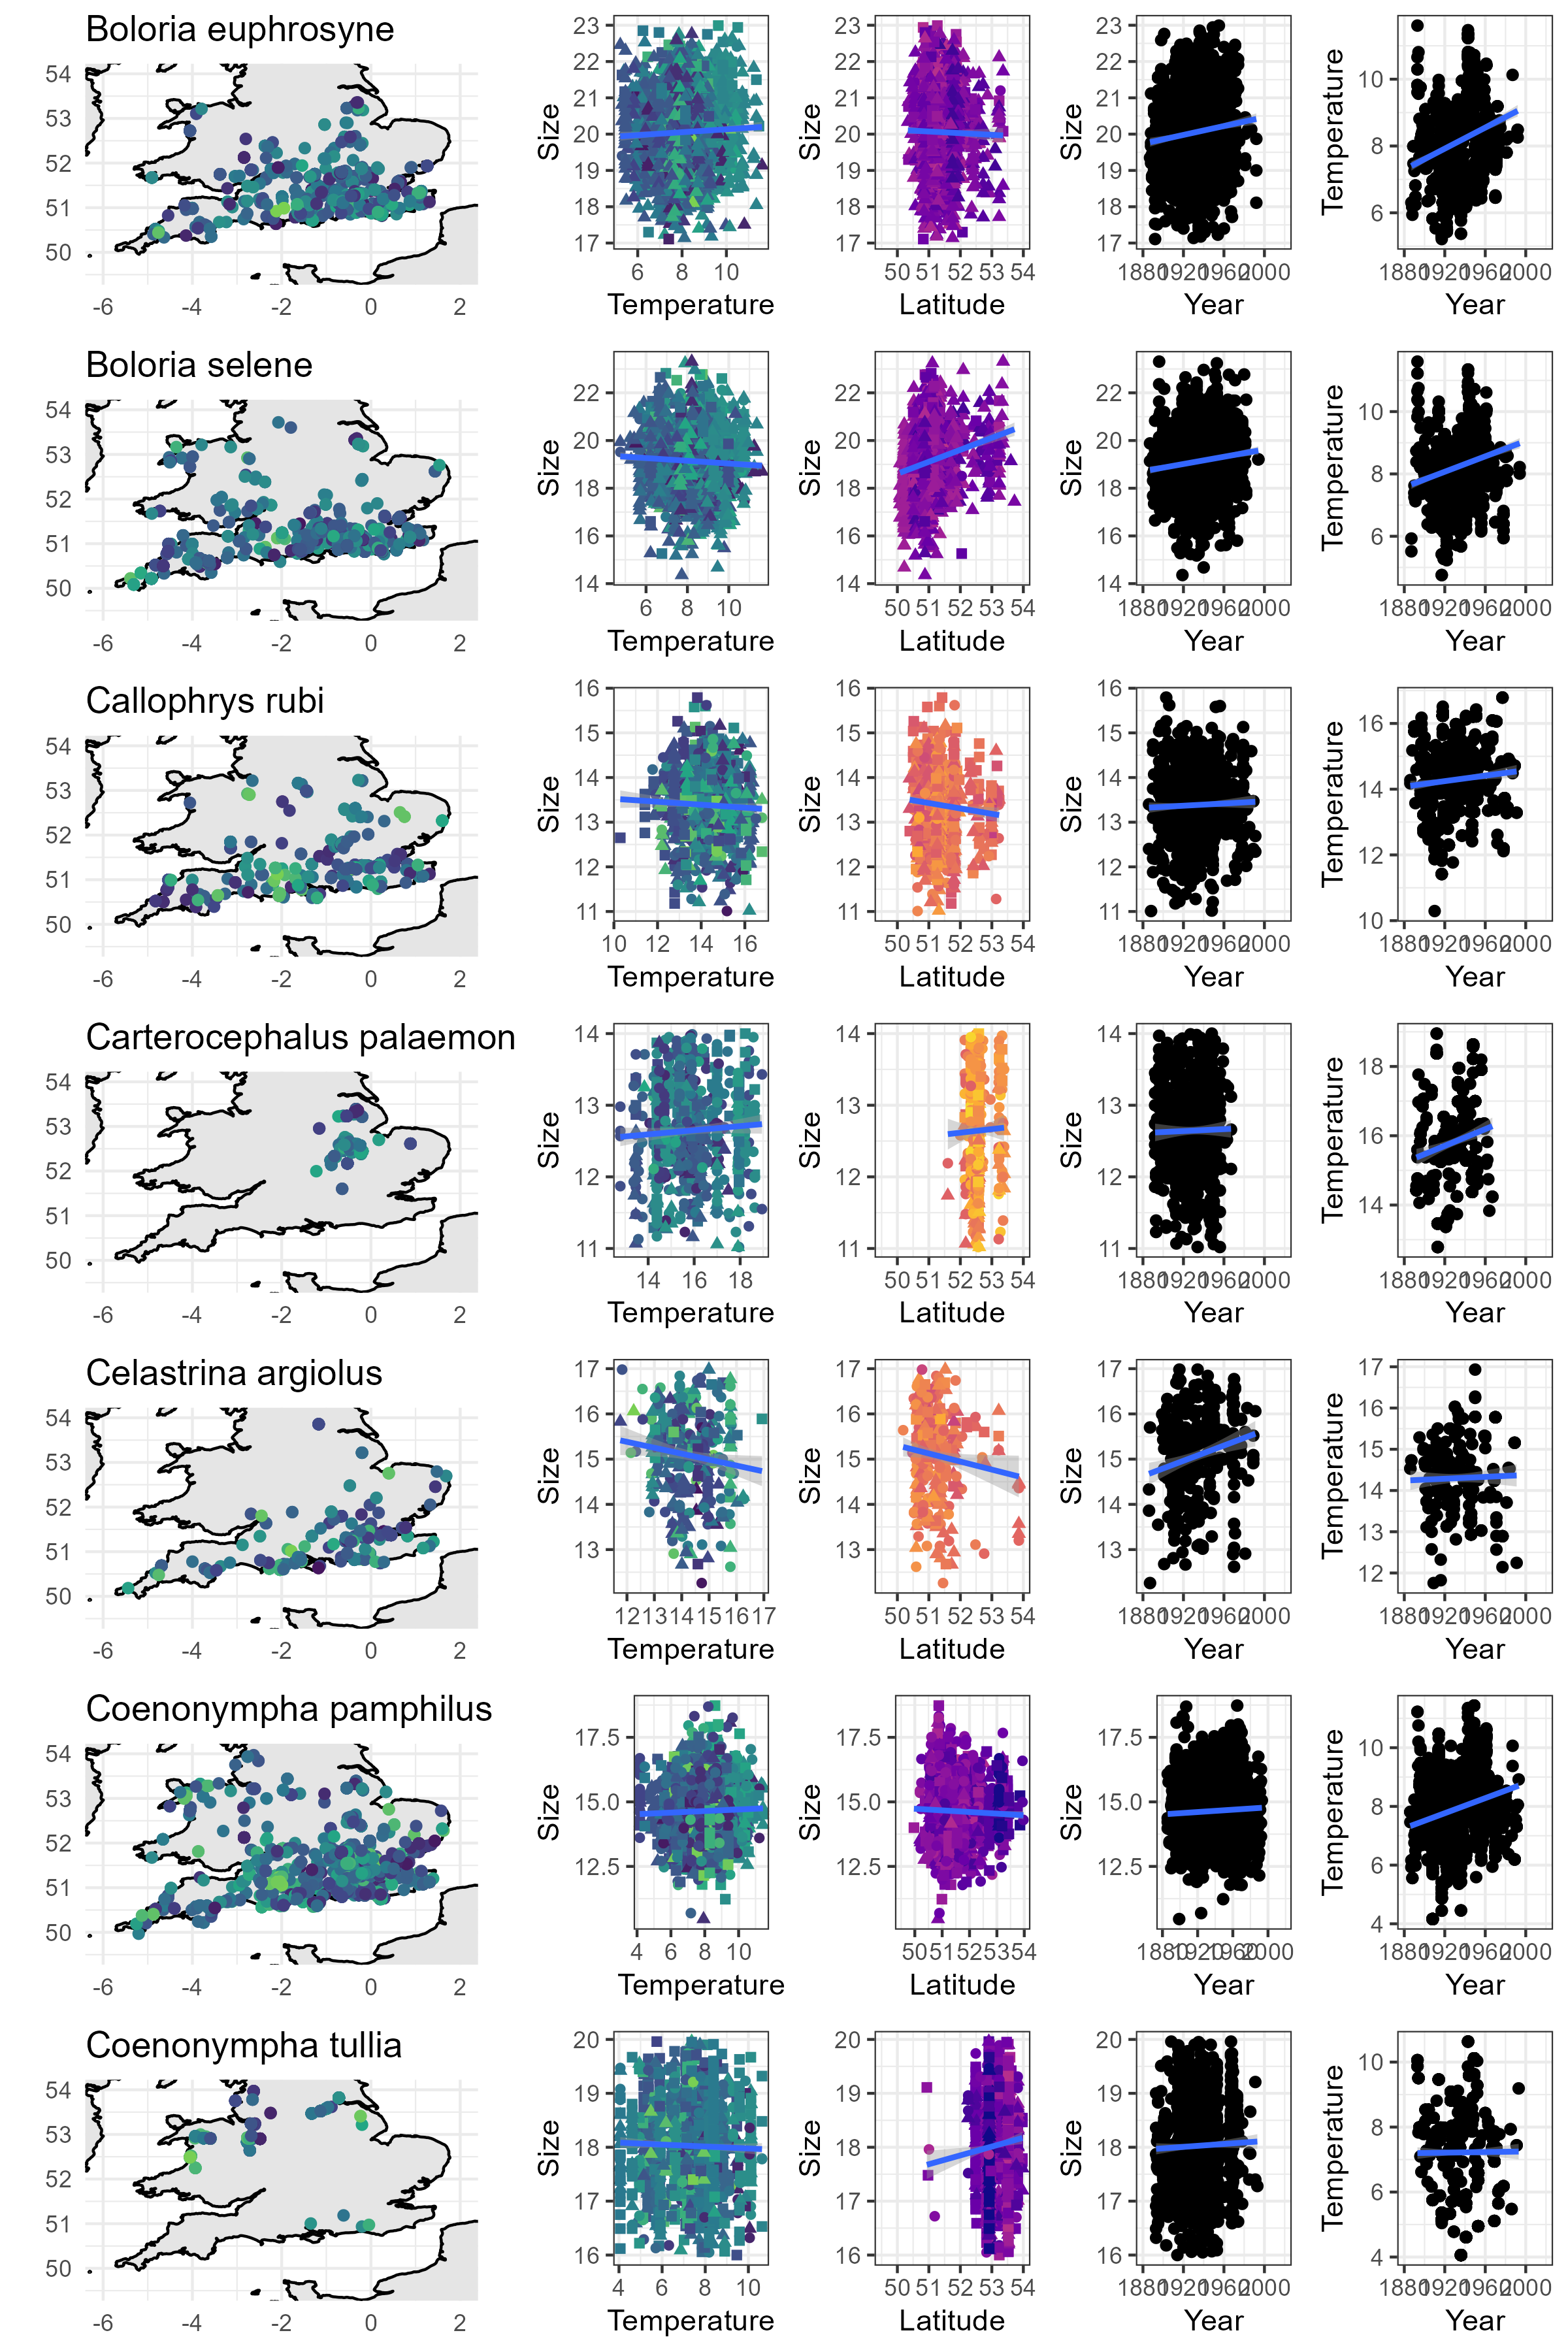
\includegraphics[width=\linewidth]{../figs/SI_NHM_dataspread_2.png}
\end{figure}
\begin{figure}[H]
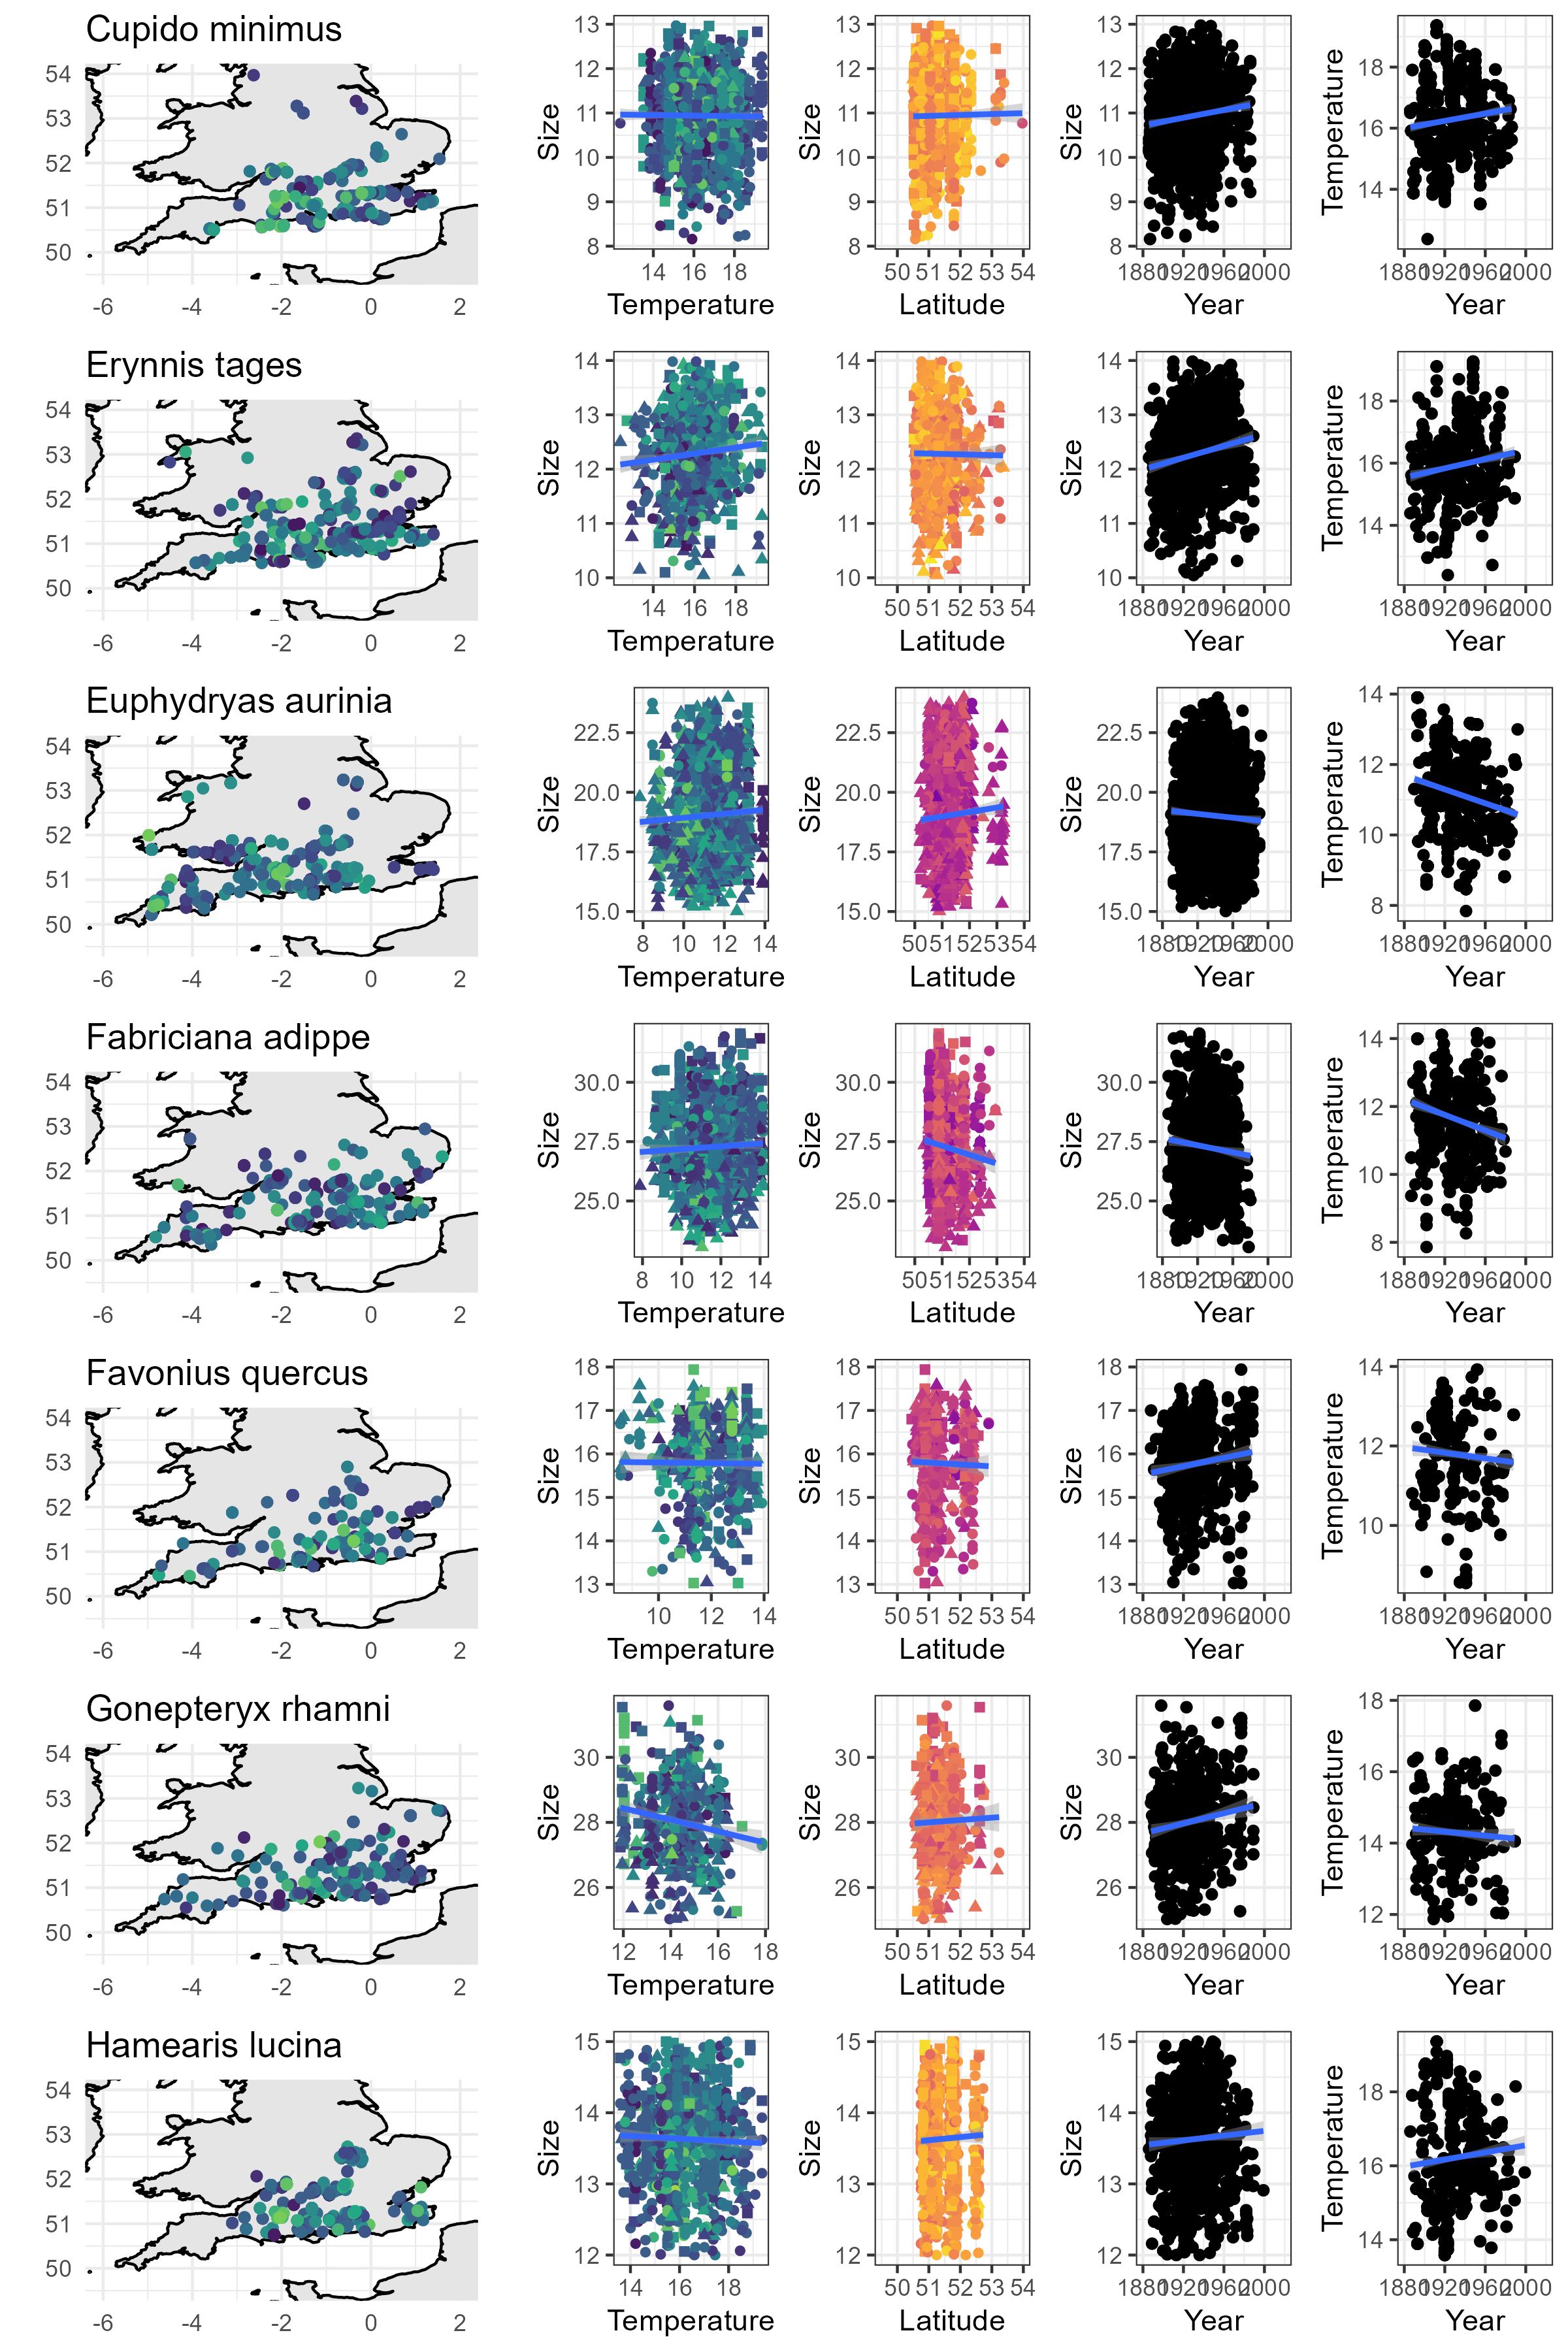
\includegraphics[width=\linewidth]{../figs/SI_NHM_dataspread_3.png}
\end{figure}
\begin{figure}[H]
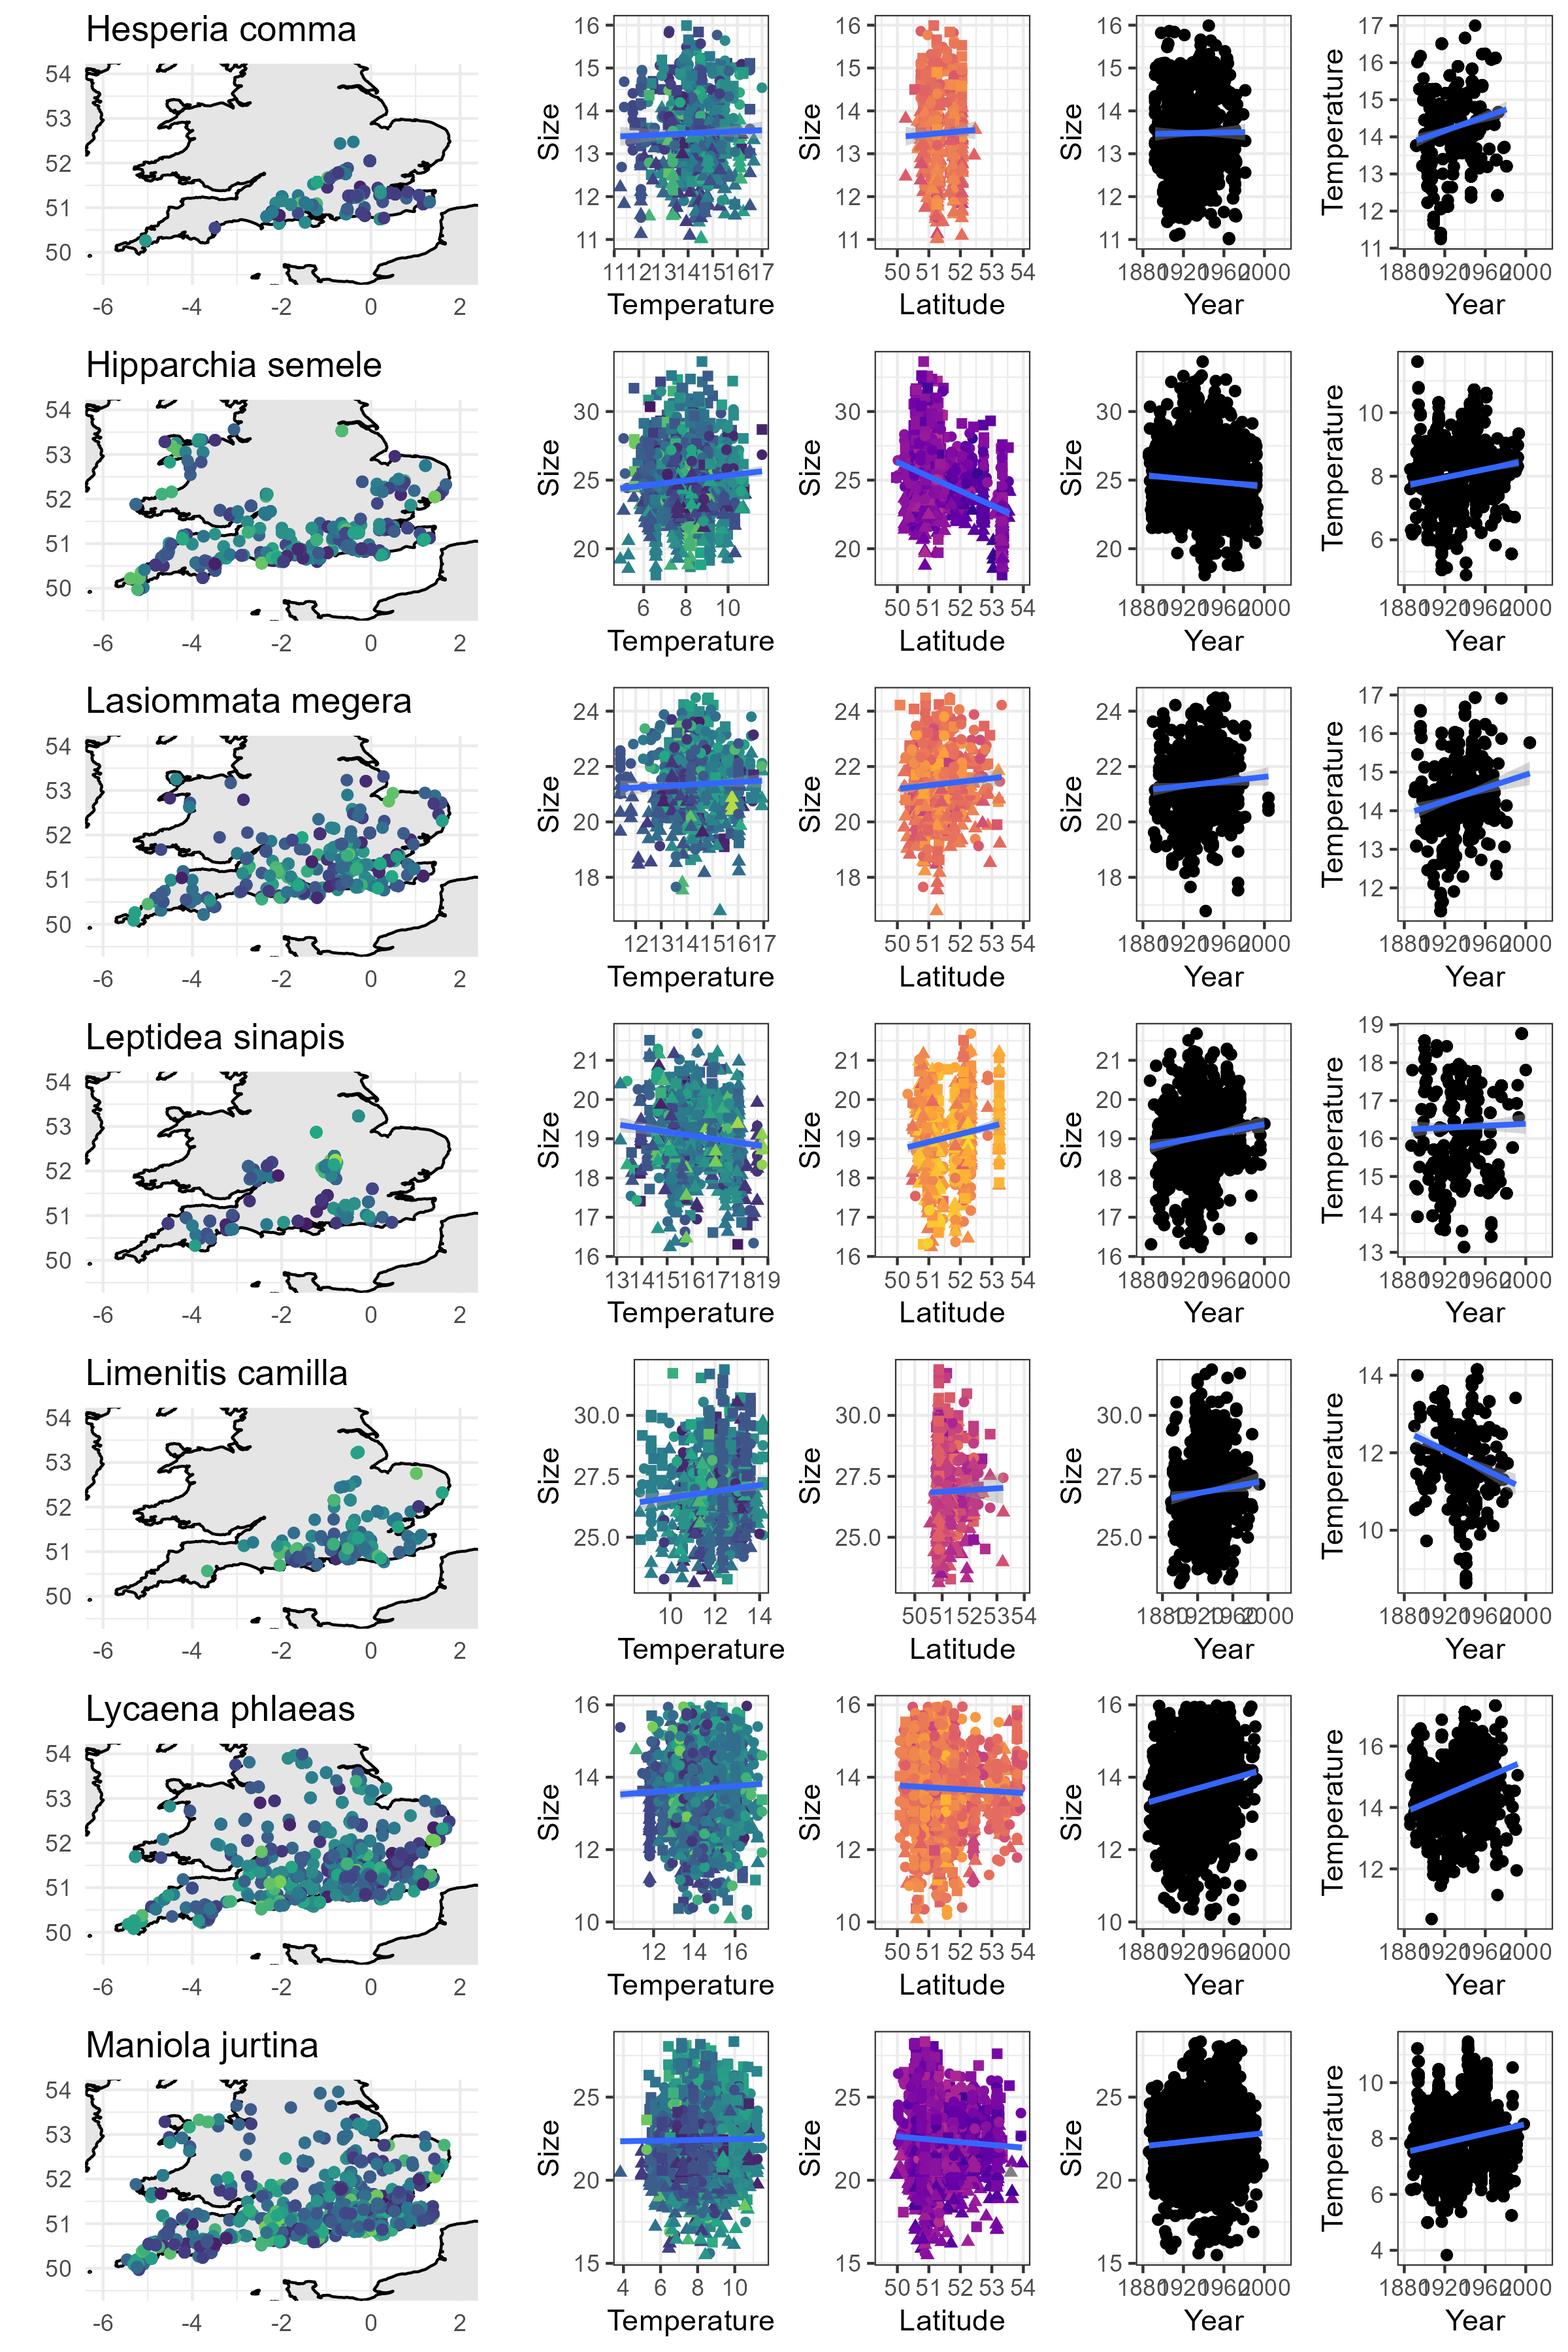
\includegraphics[width=\linewidth]{../figs/SI_NHM_dataspread_4.png}
\end{figure}
\begin{figure}[H]
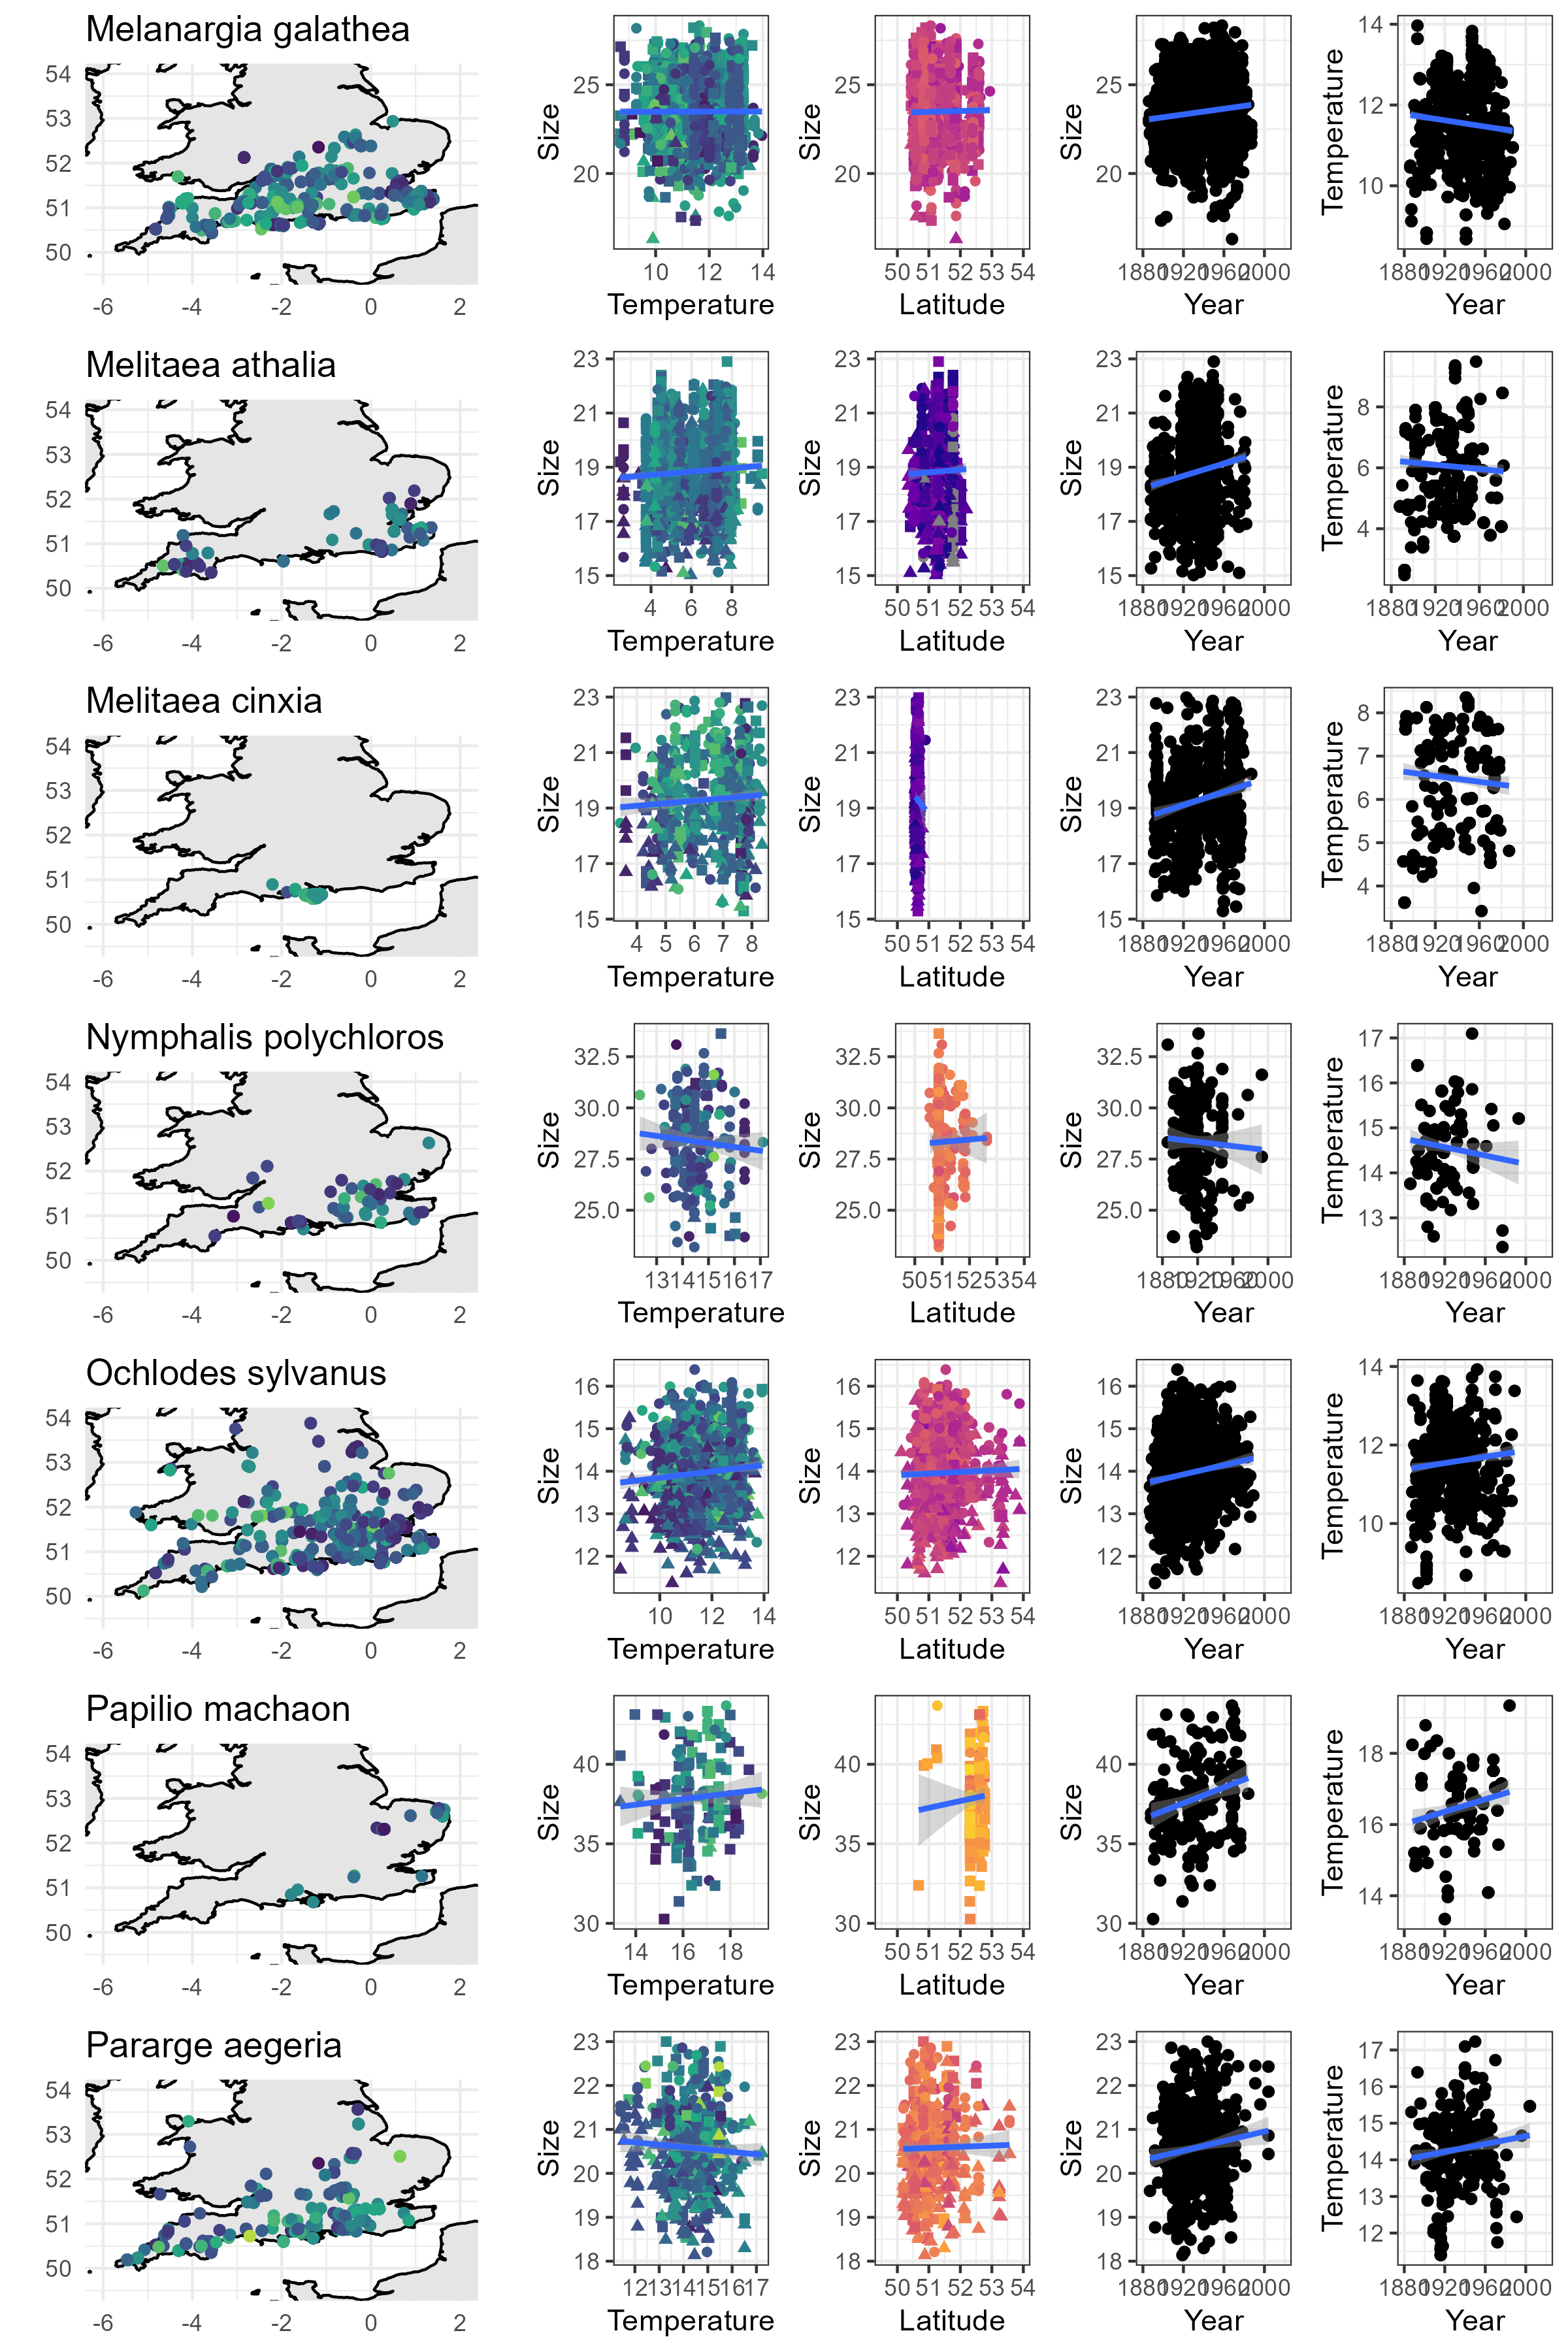
\includegraphics[width=\linewidth]{../figs/SI_NHM_dataspread_5.png}
\end{figure}
\begin{figure}[H]
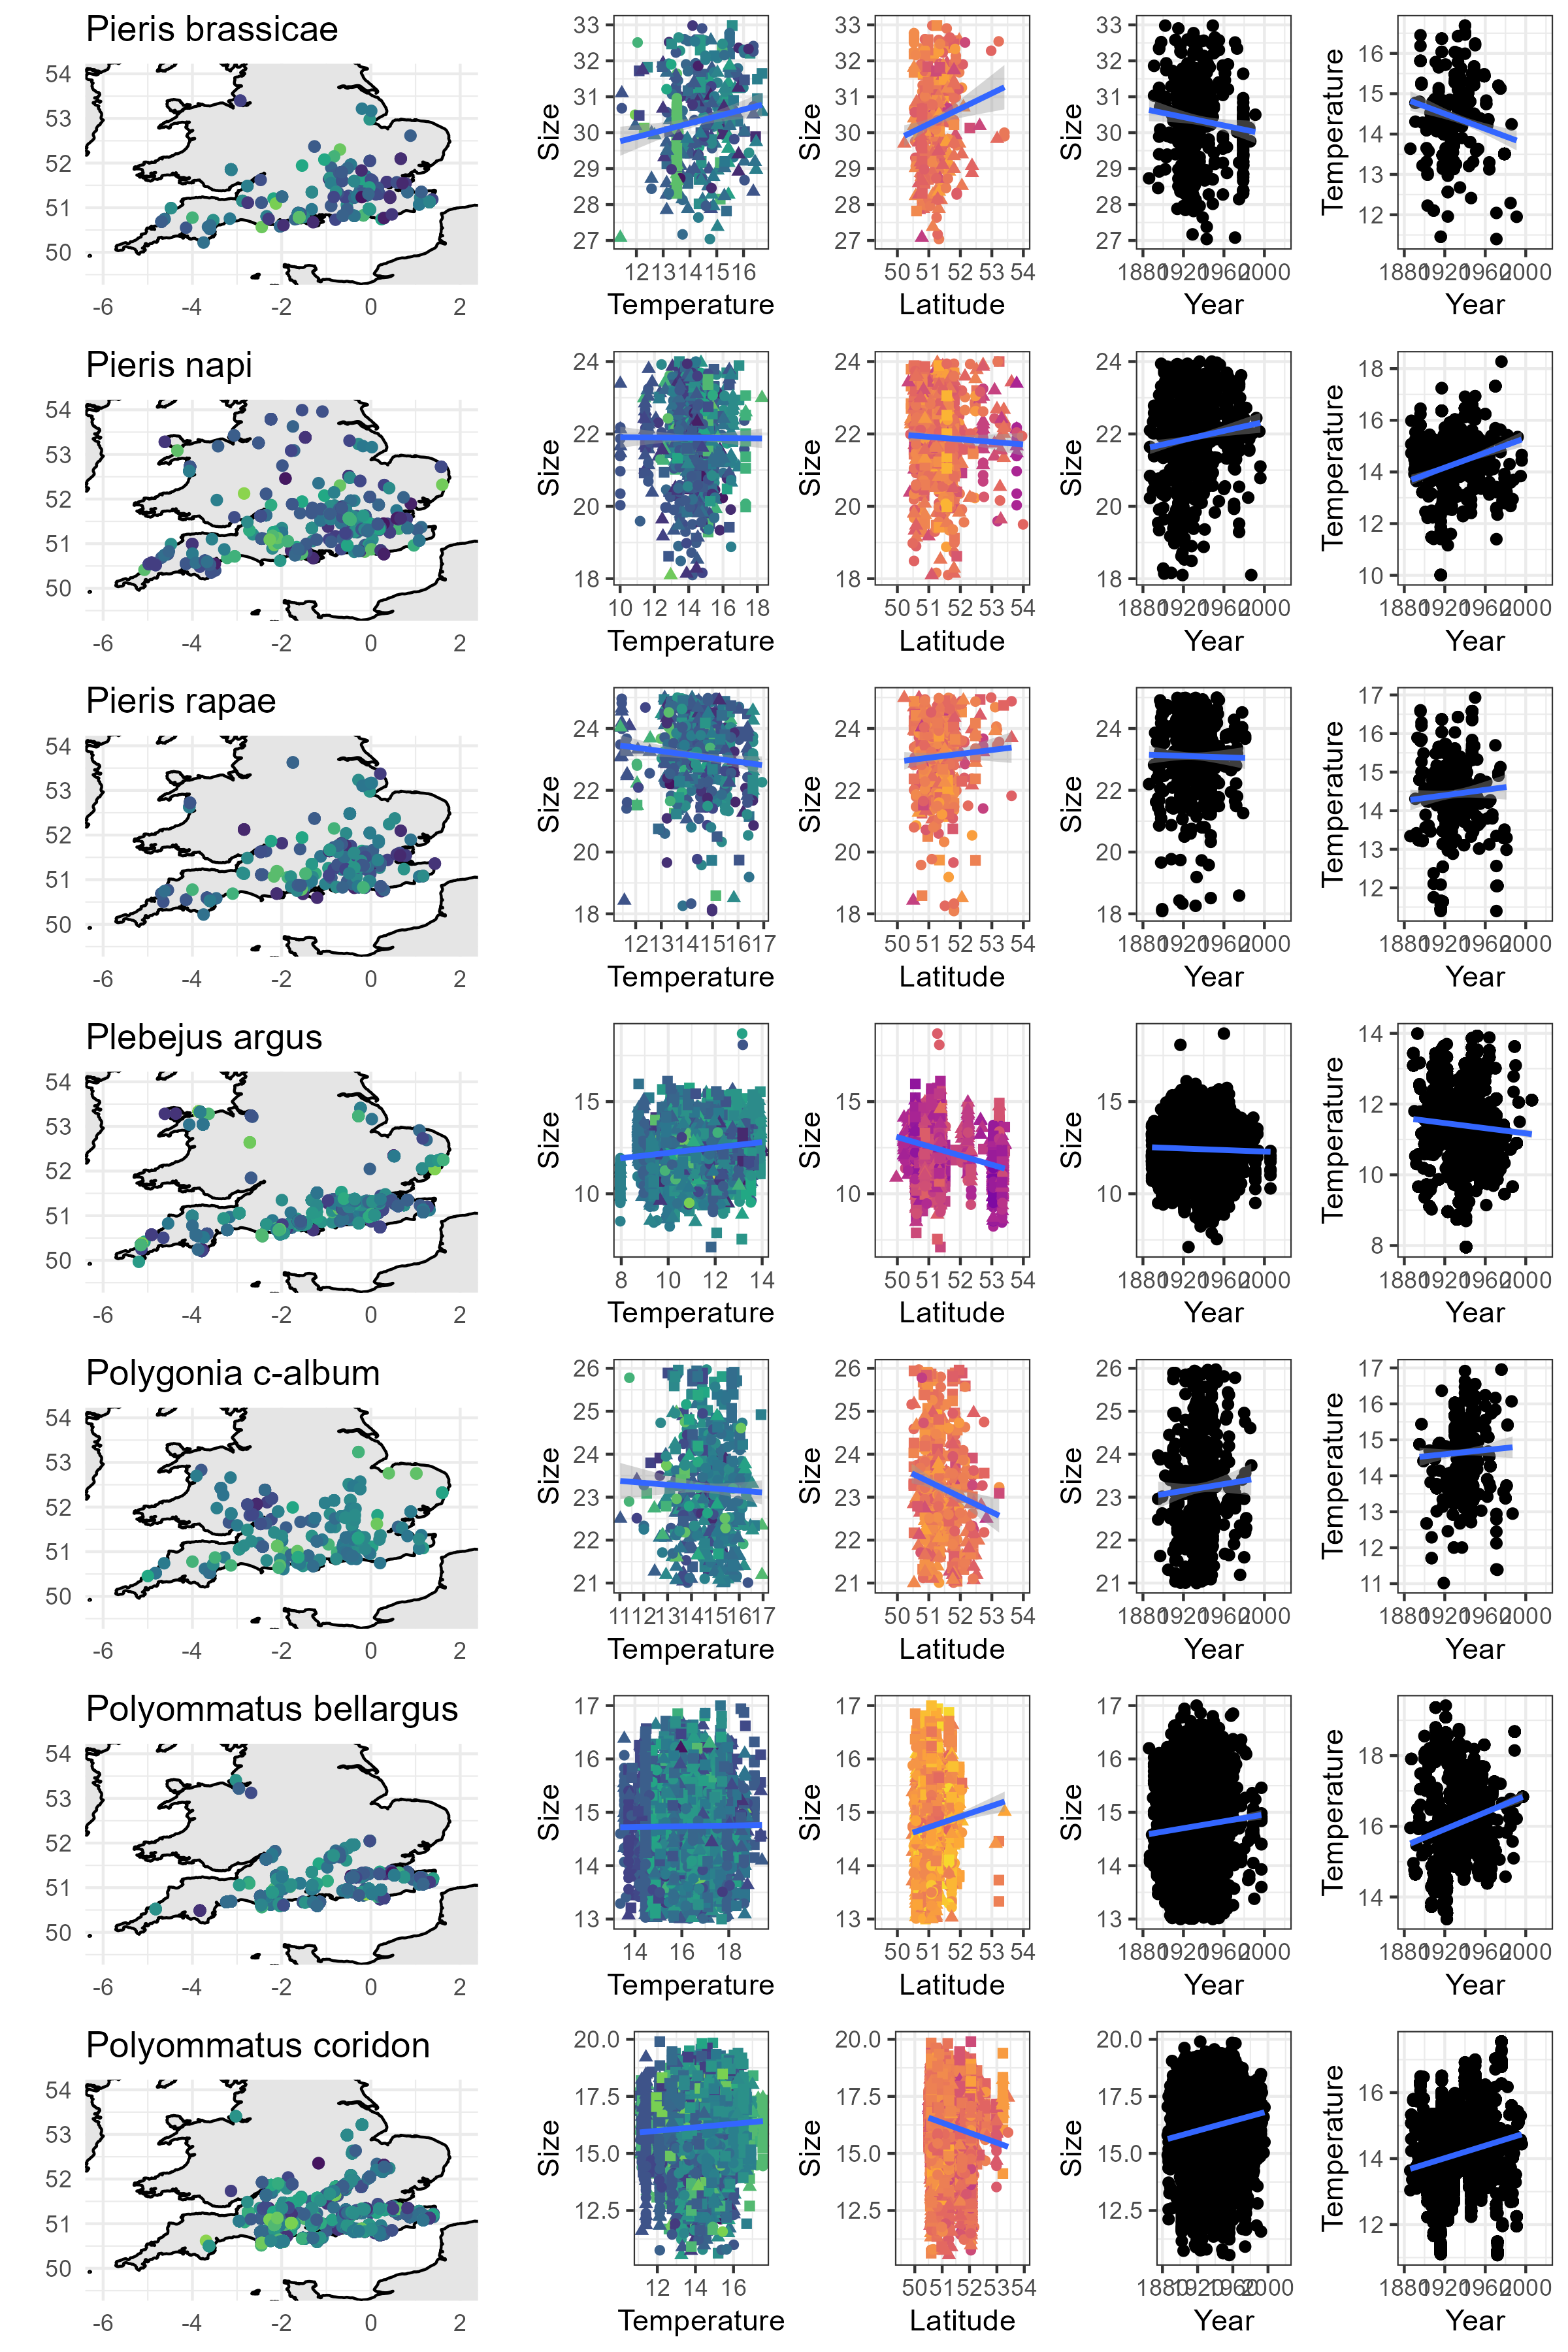
\includegraphics[width=\linewidth]{../figs/SI_NHM_dataspread_6.png}
\end{figure}
\begin{figure}[H]
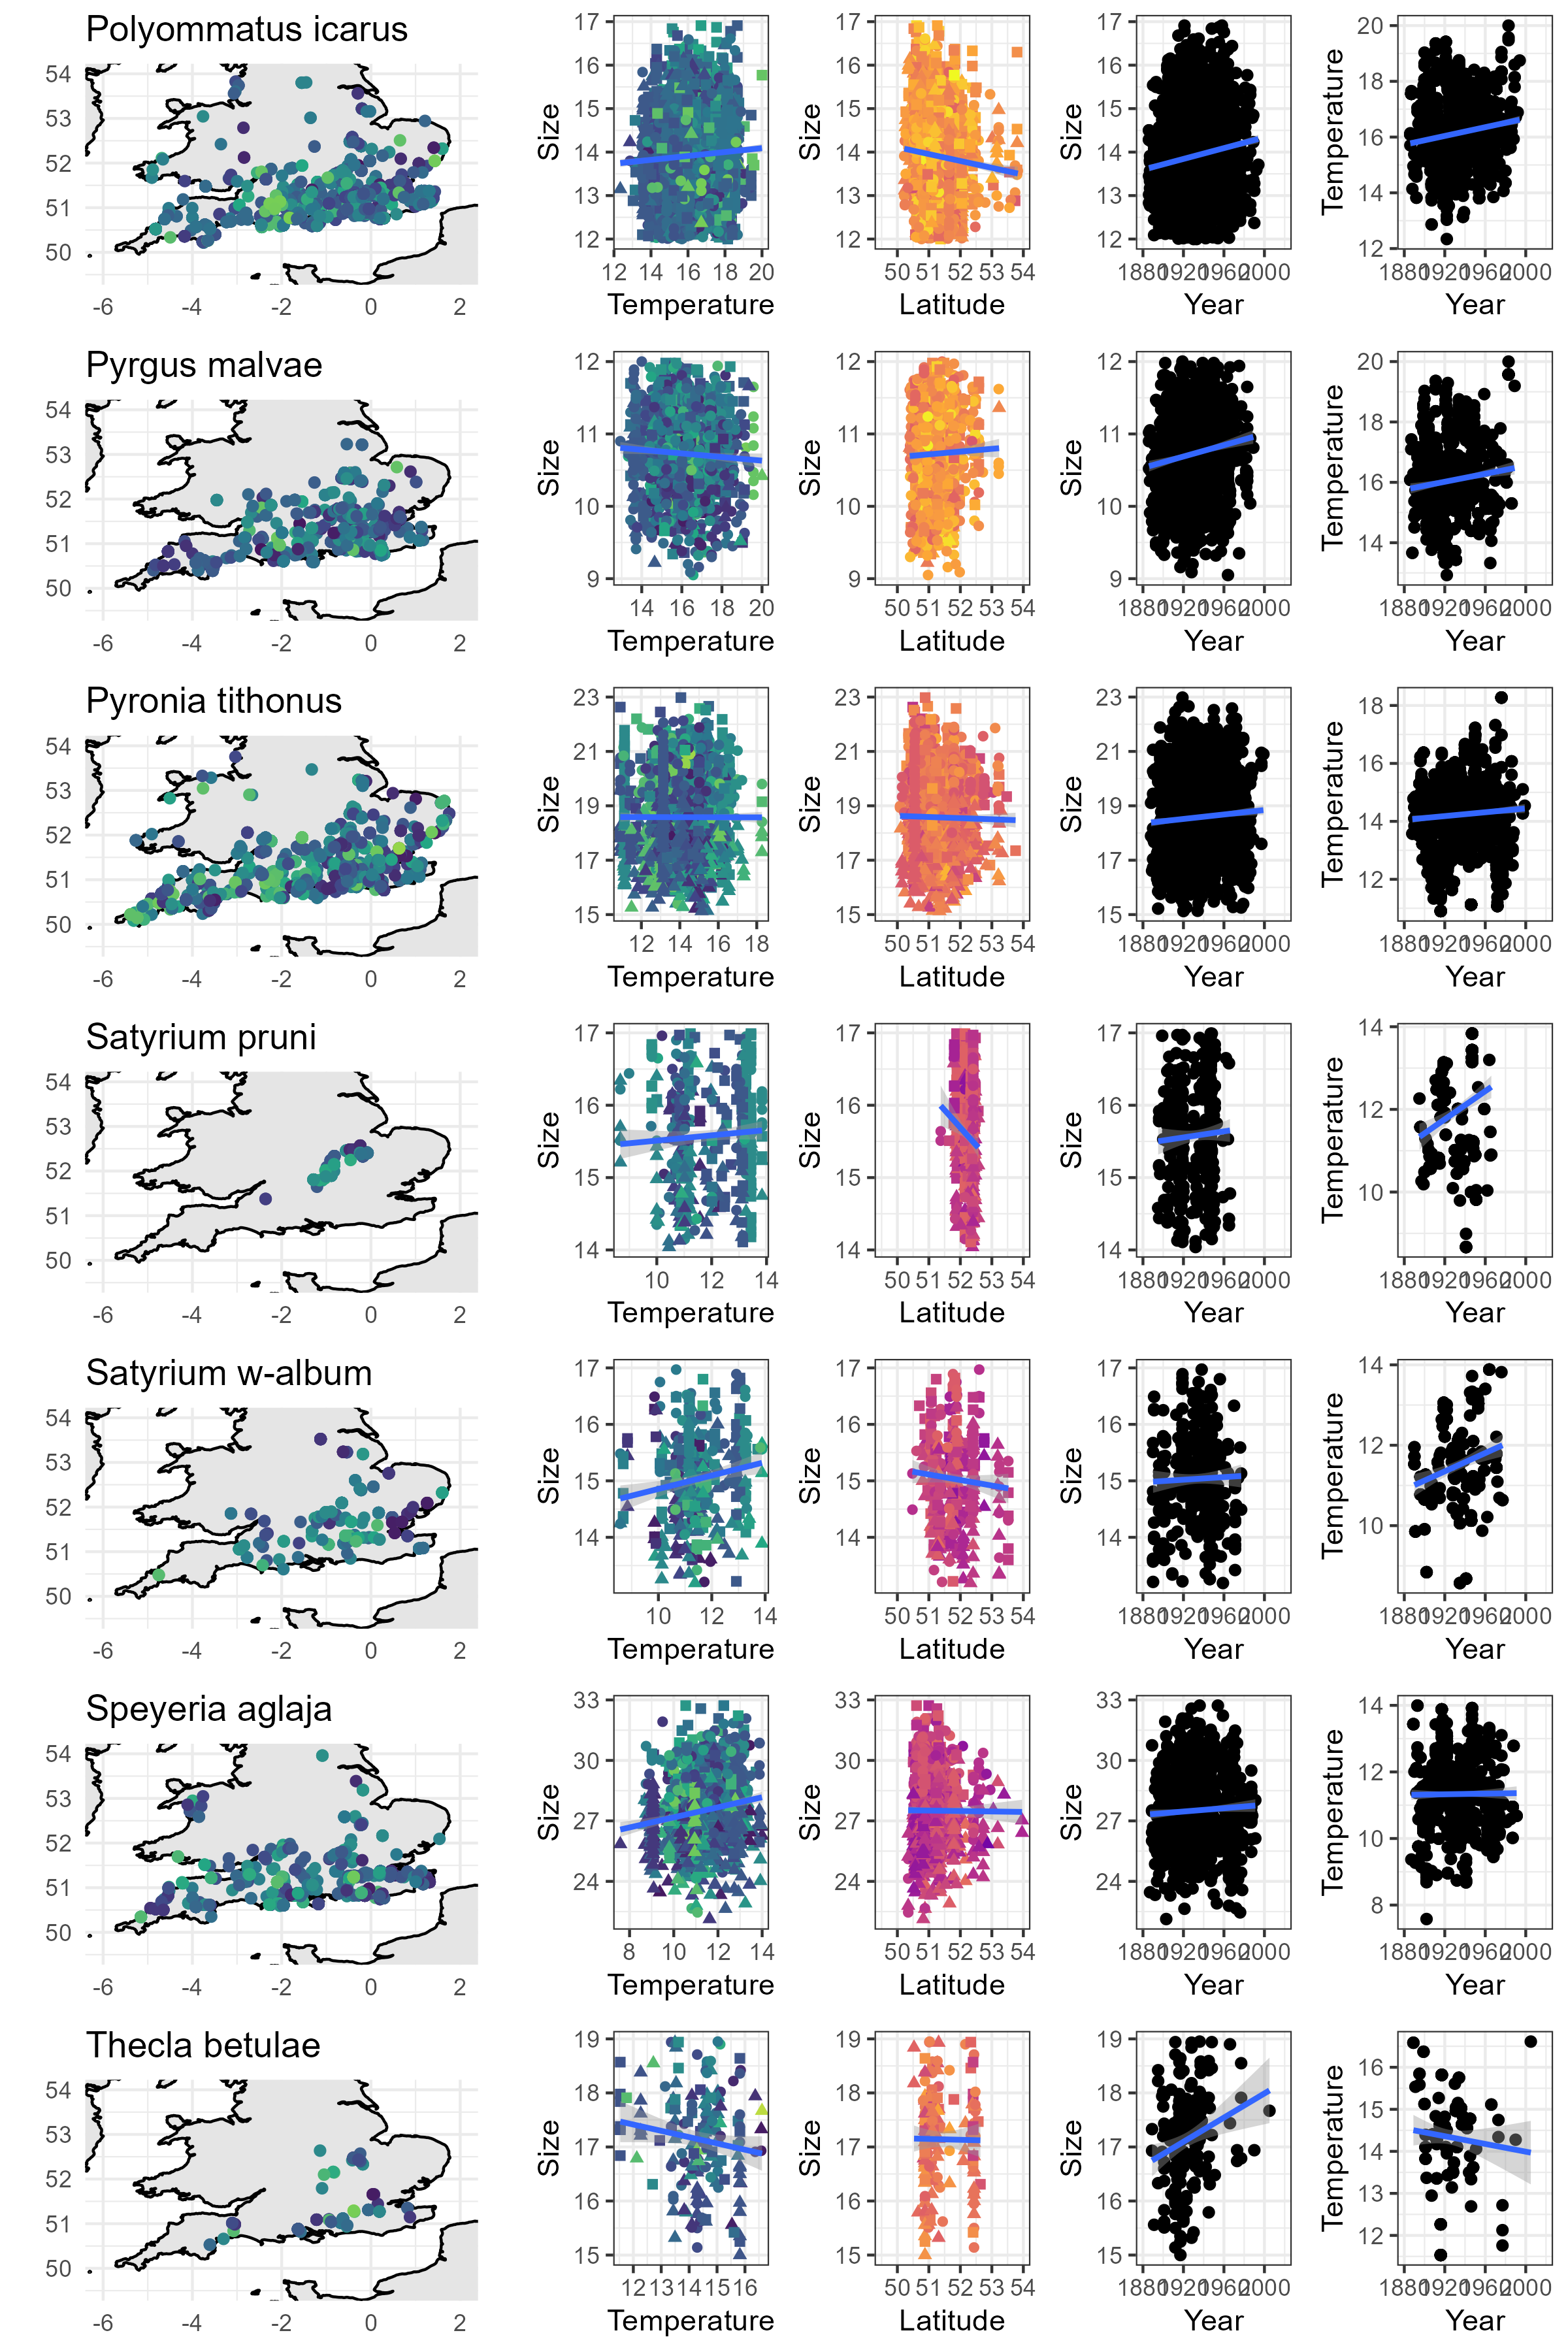
\includegraphics[width=\linewidth]{../figs/SI_NHM_dataspread_7.png}
\end{figure}
\begin{figure}[H]
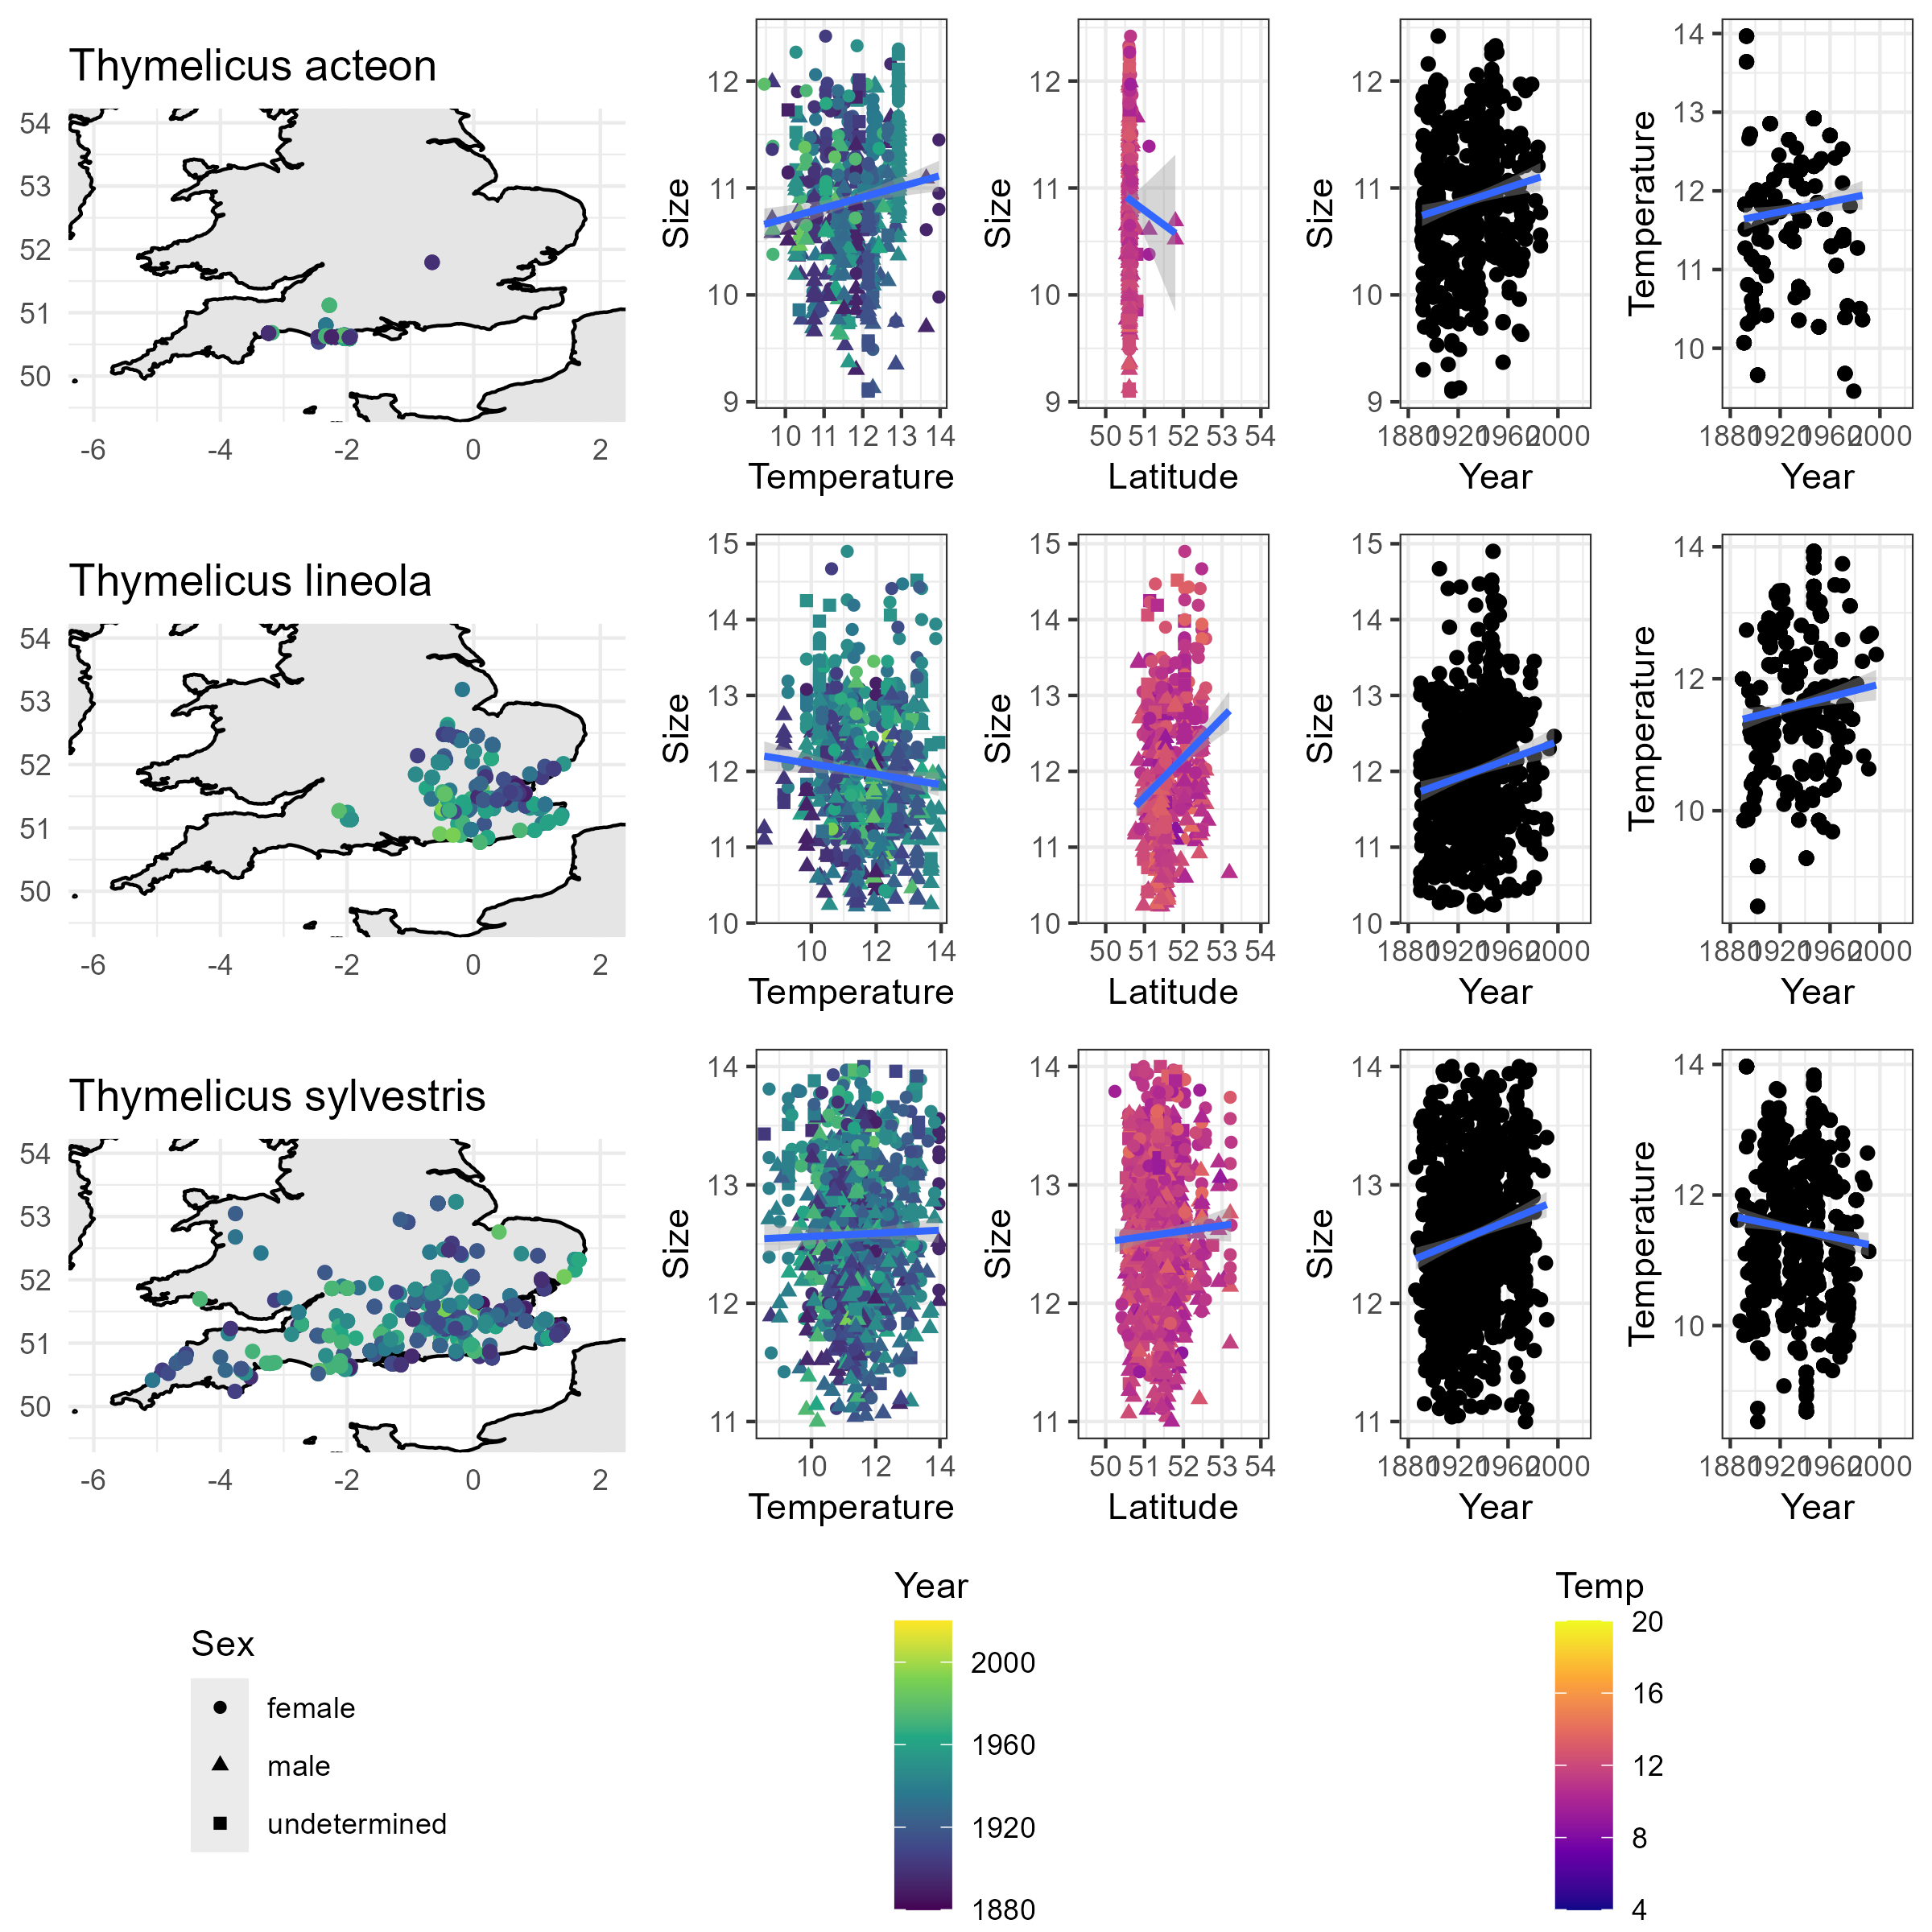
\includegraphics[width=\linewidth]{../figs/SI_NHM_dataspread_8.png}
\end{figure}

\textbf{Figure S10: Distribution of records (post-filtering) from the NHM dataset for each species}

% Ox Data Distributions
\newpage

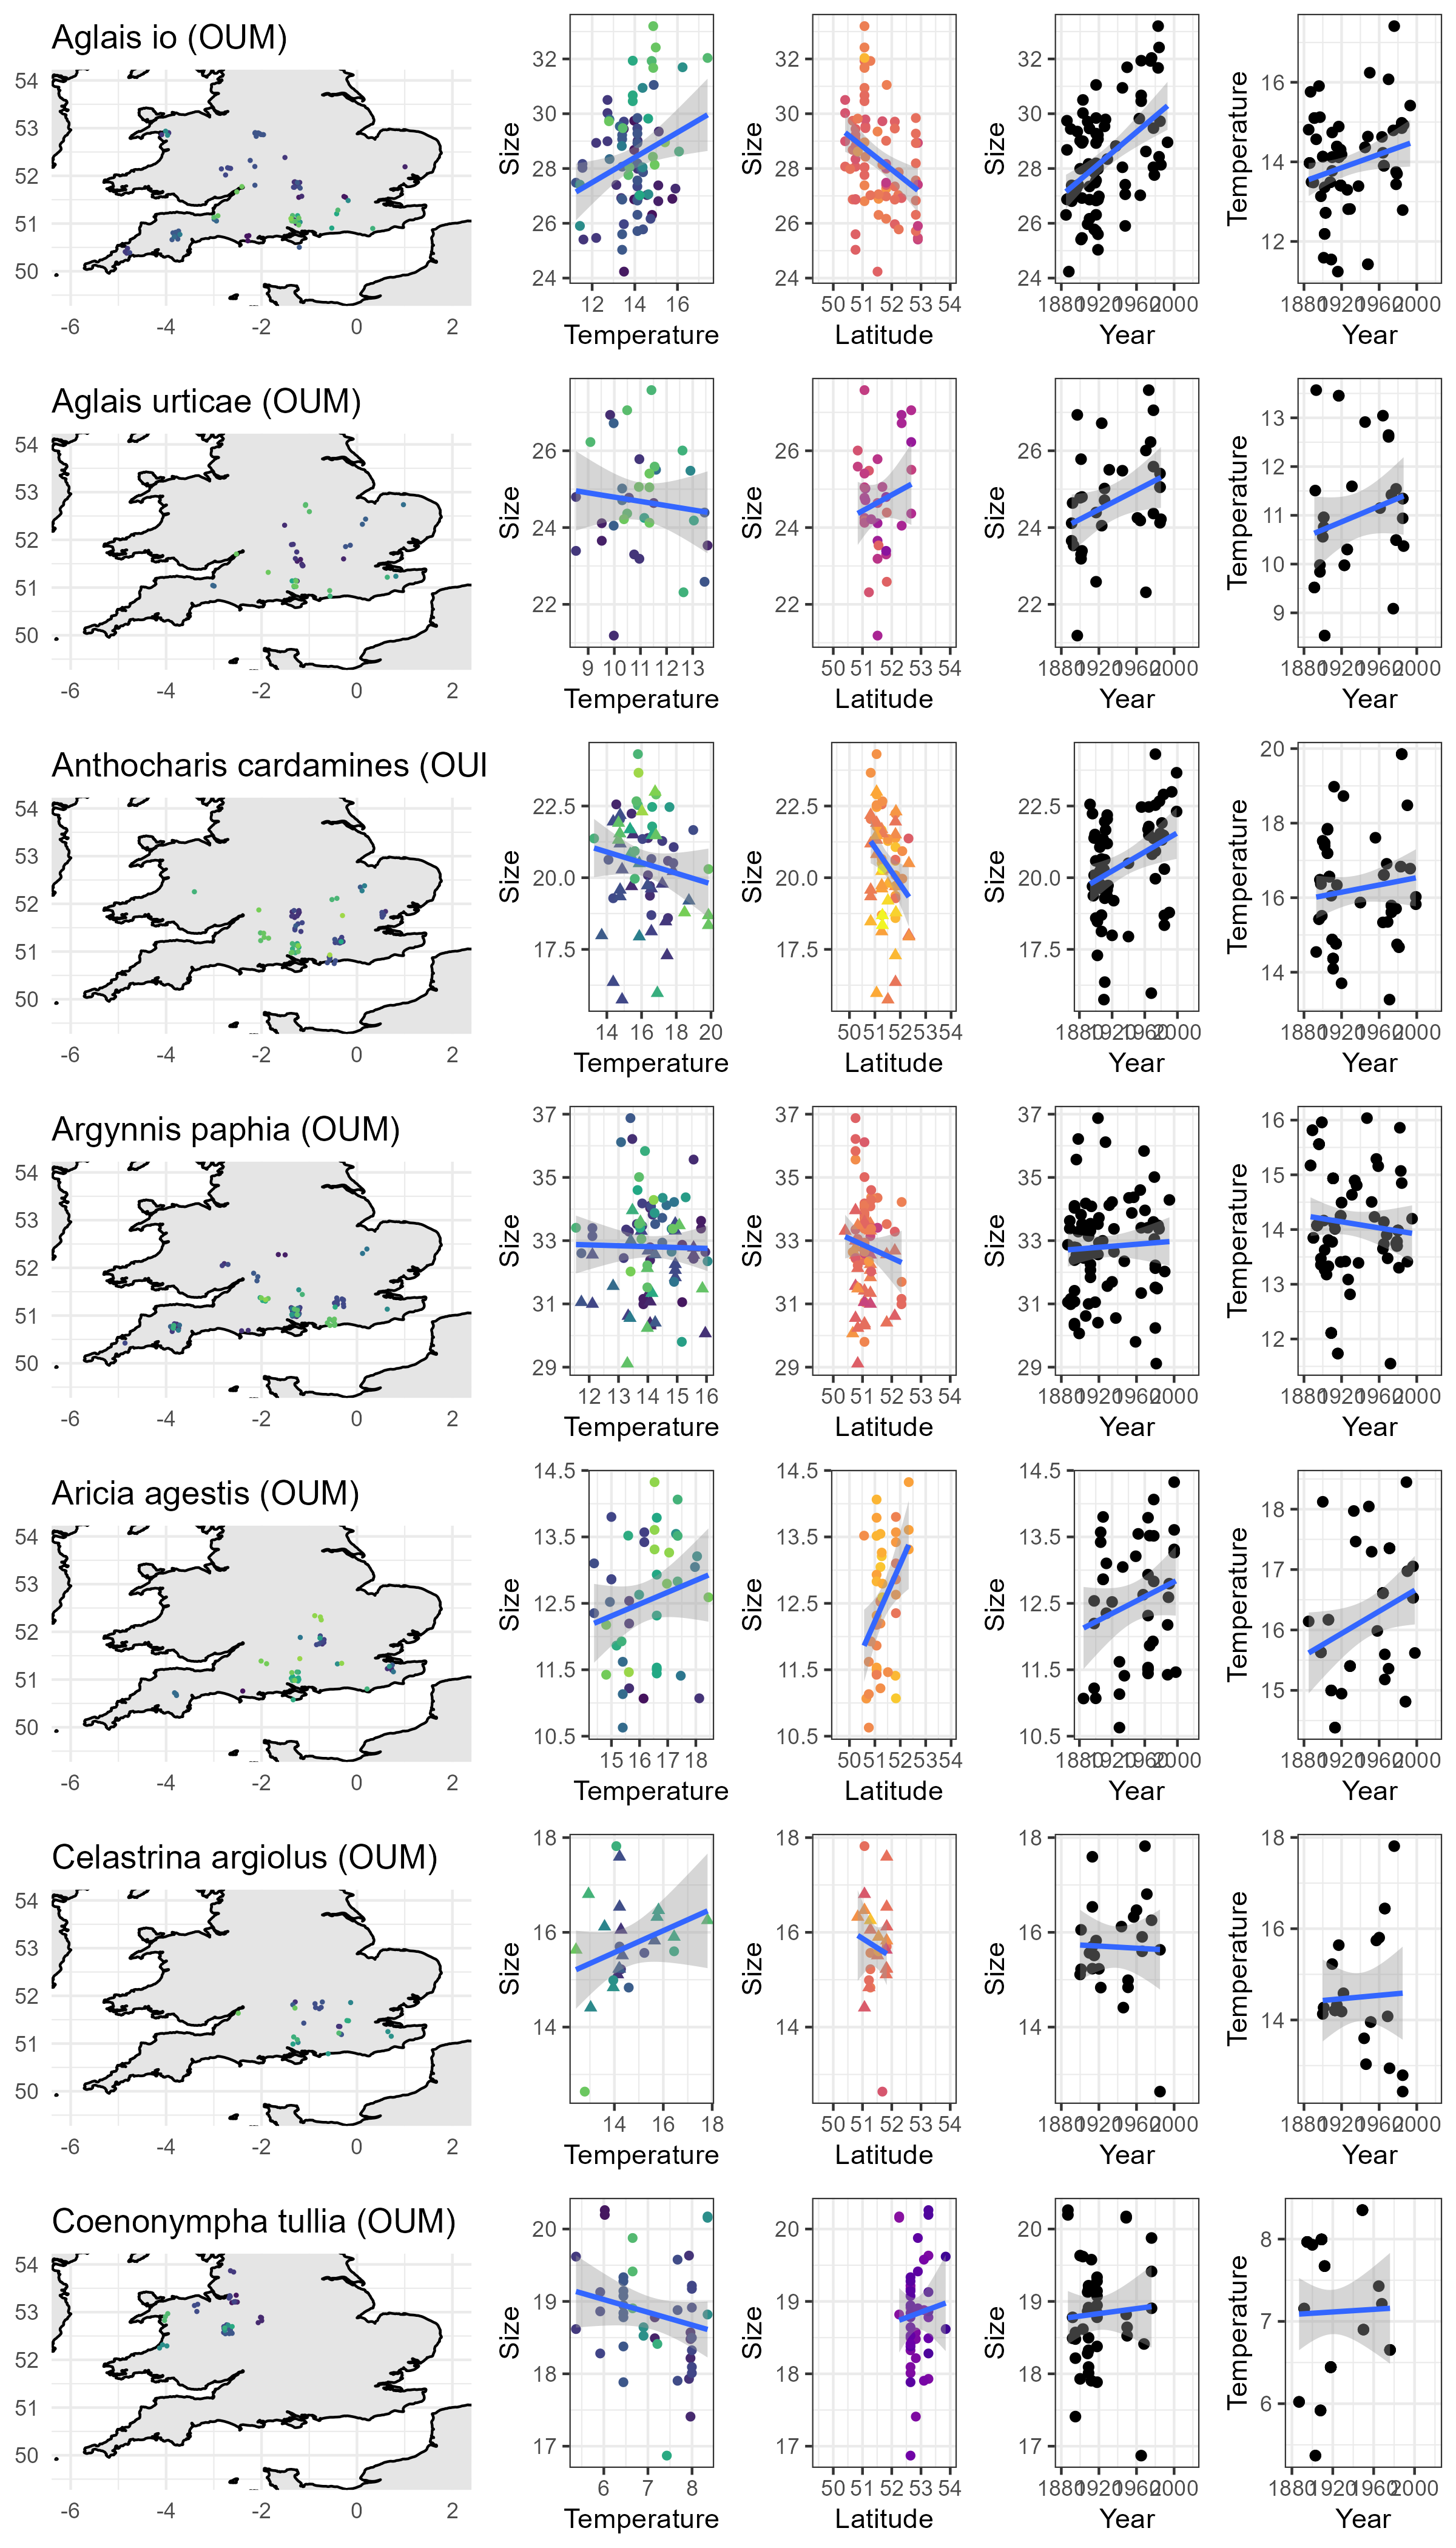
\includegraphics[width=\linewidth]{../figs/SI_OUM_dataspread_1.png}
\begin{figure}[H]
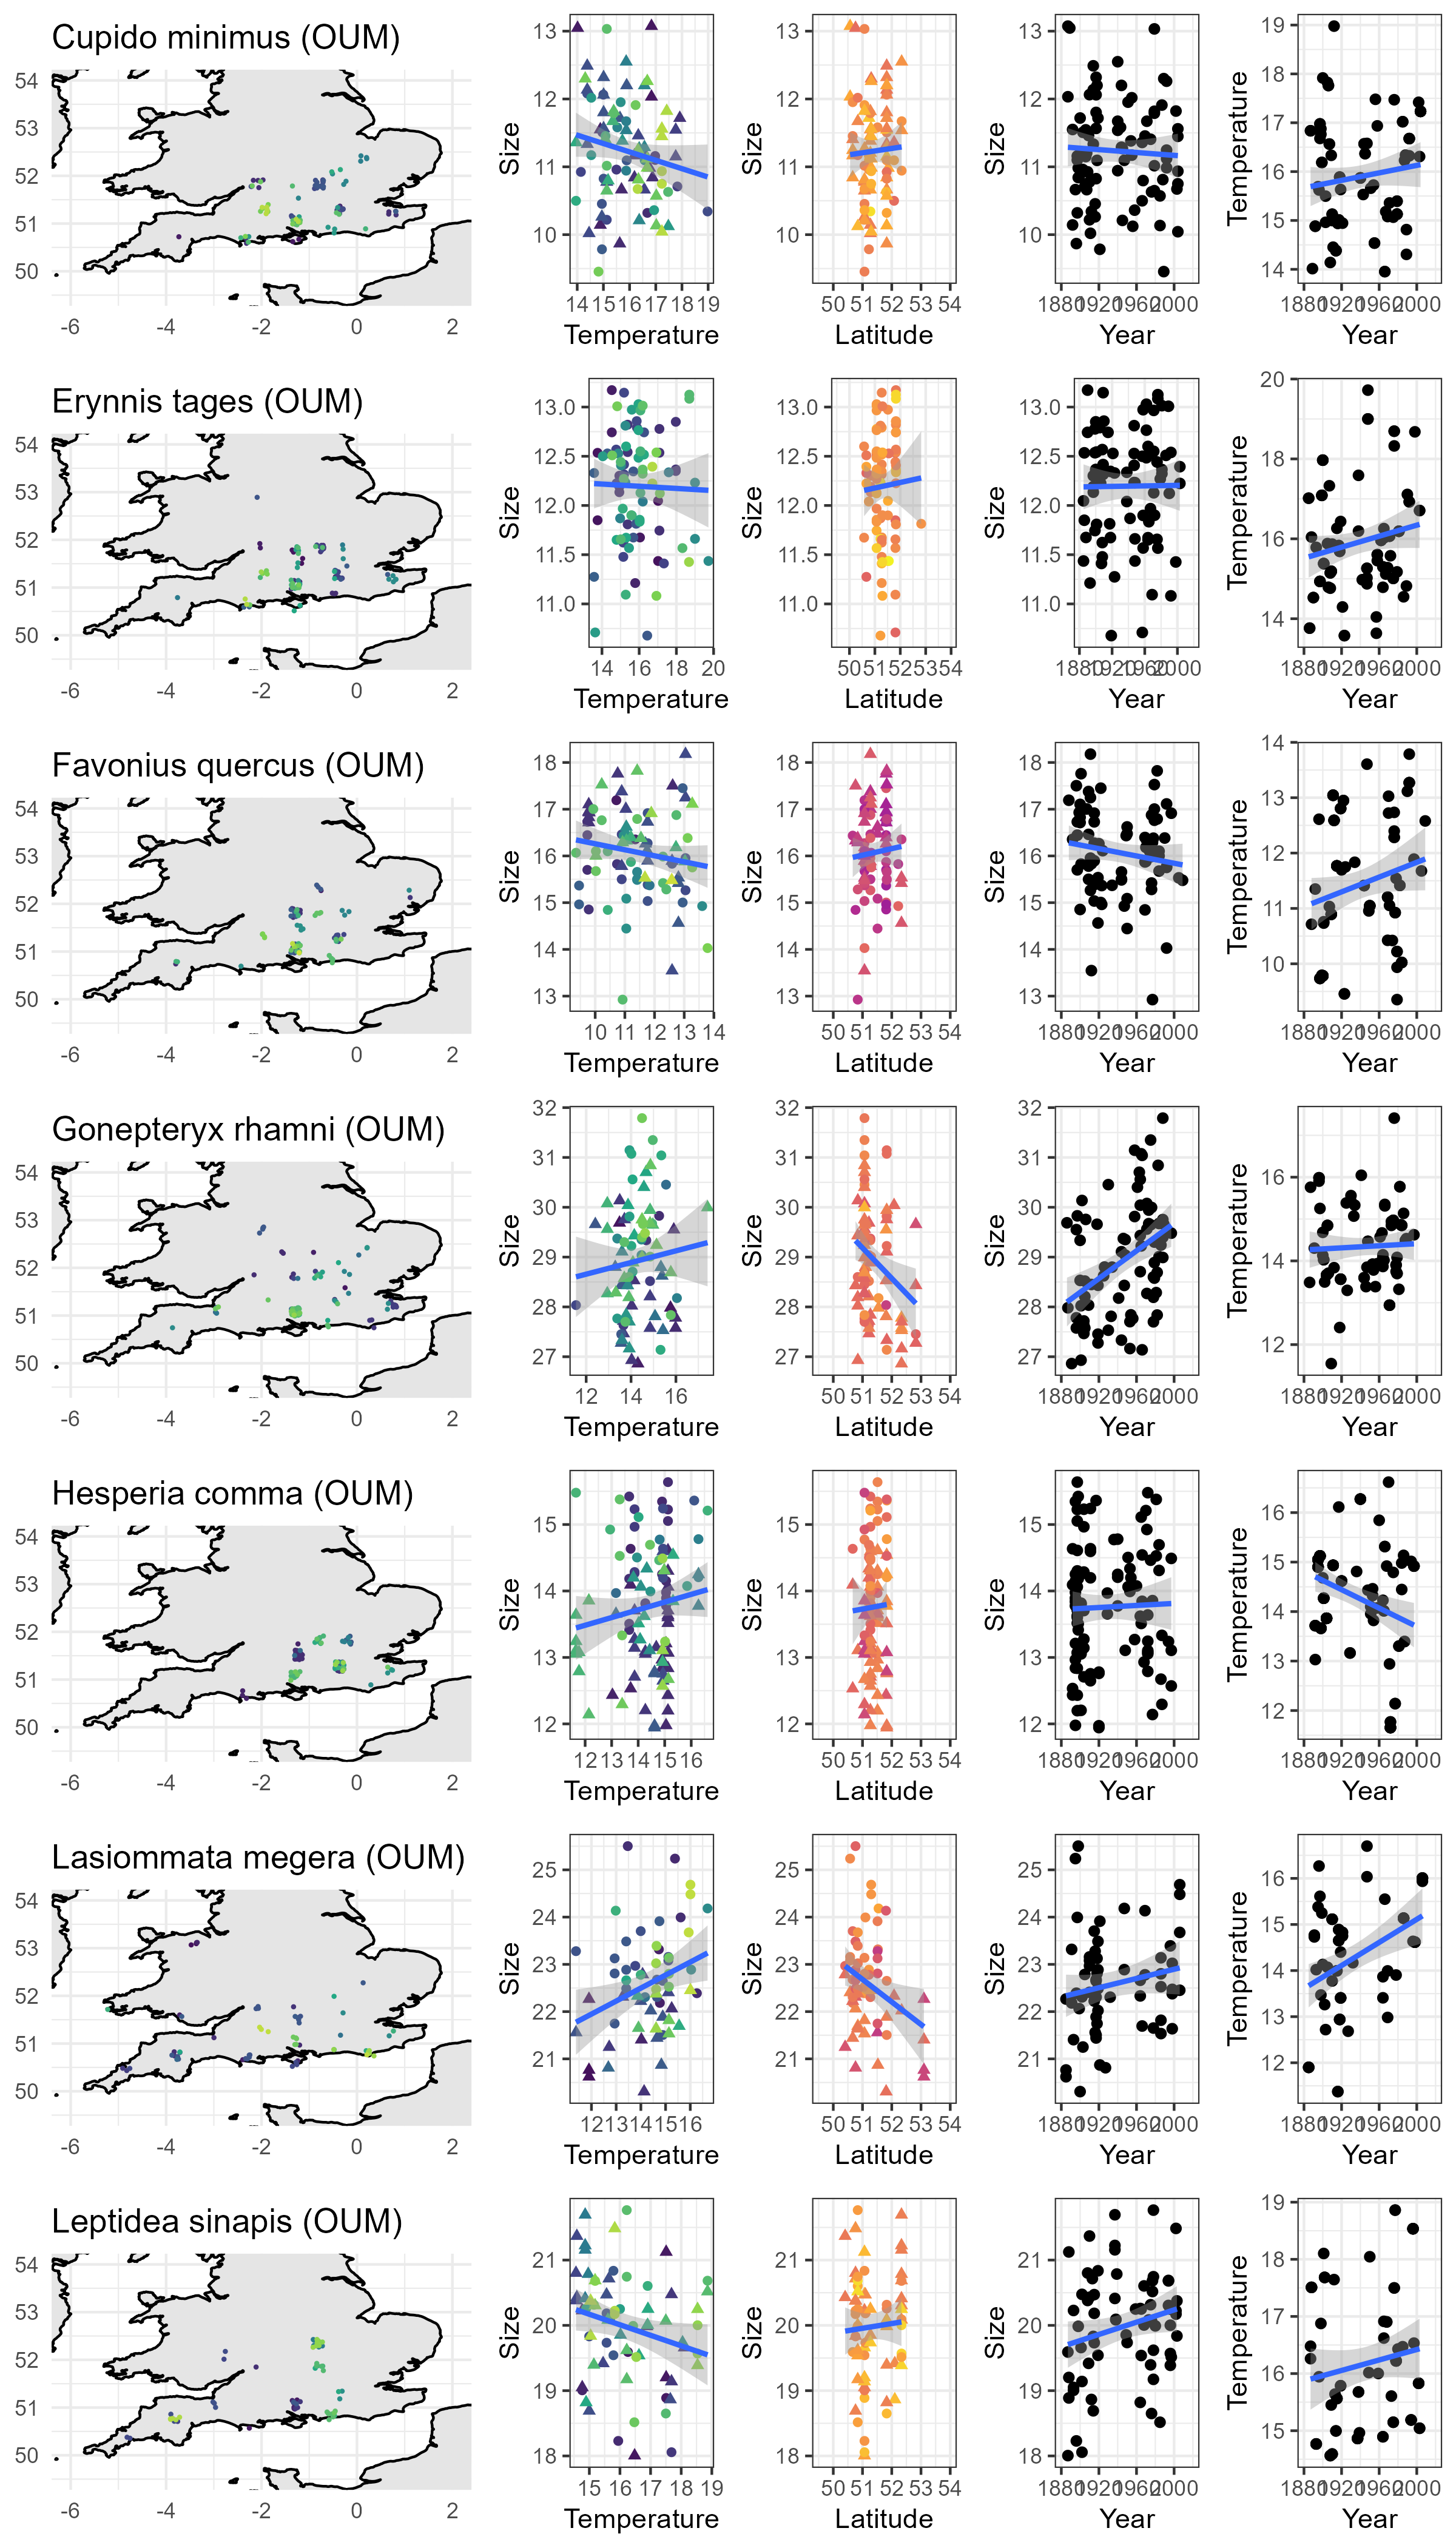
\includegraphics[width=\linewidth]{../figs/SI_OUM_dataspread_2.png}
\end{figure}
\begin{figure}[H]
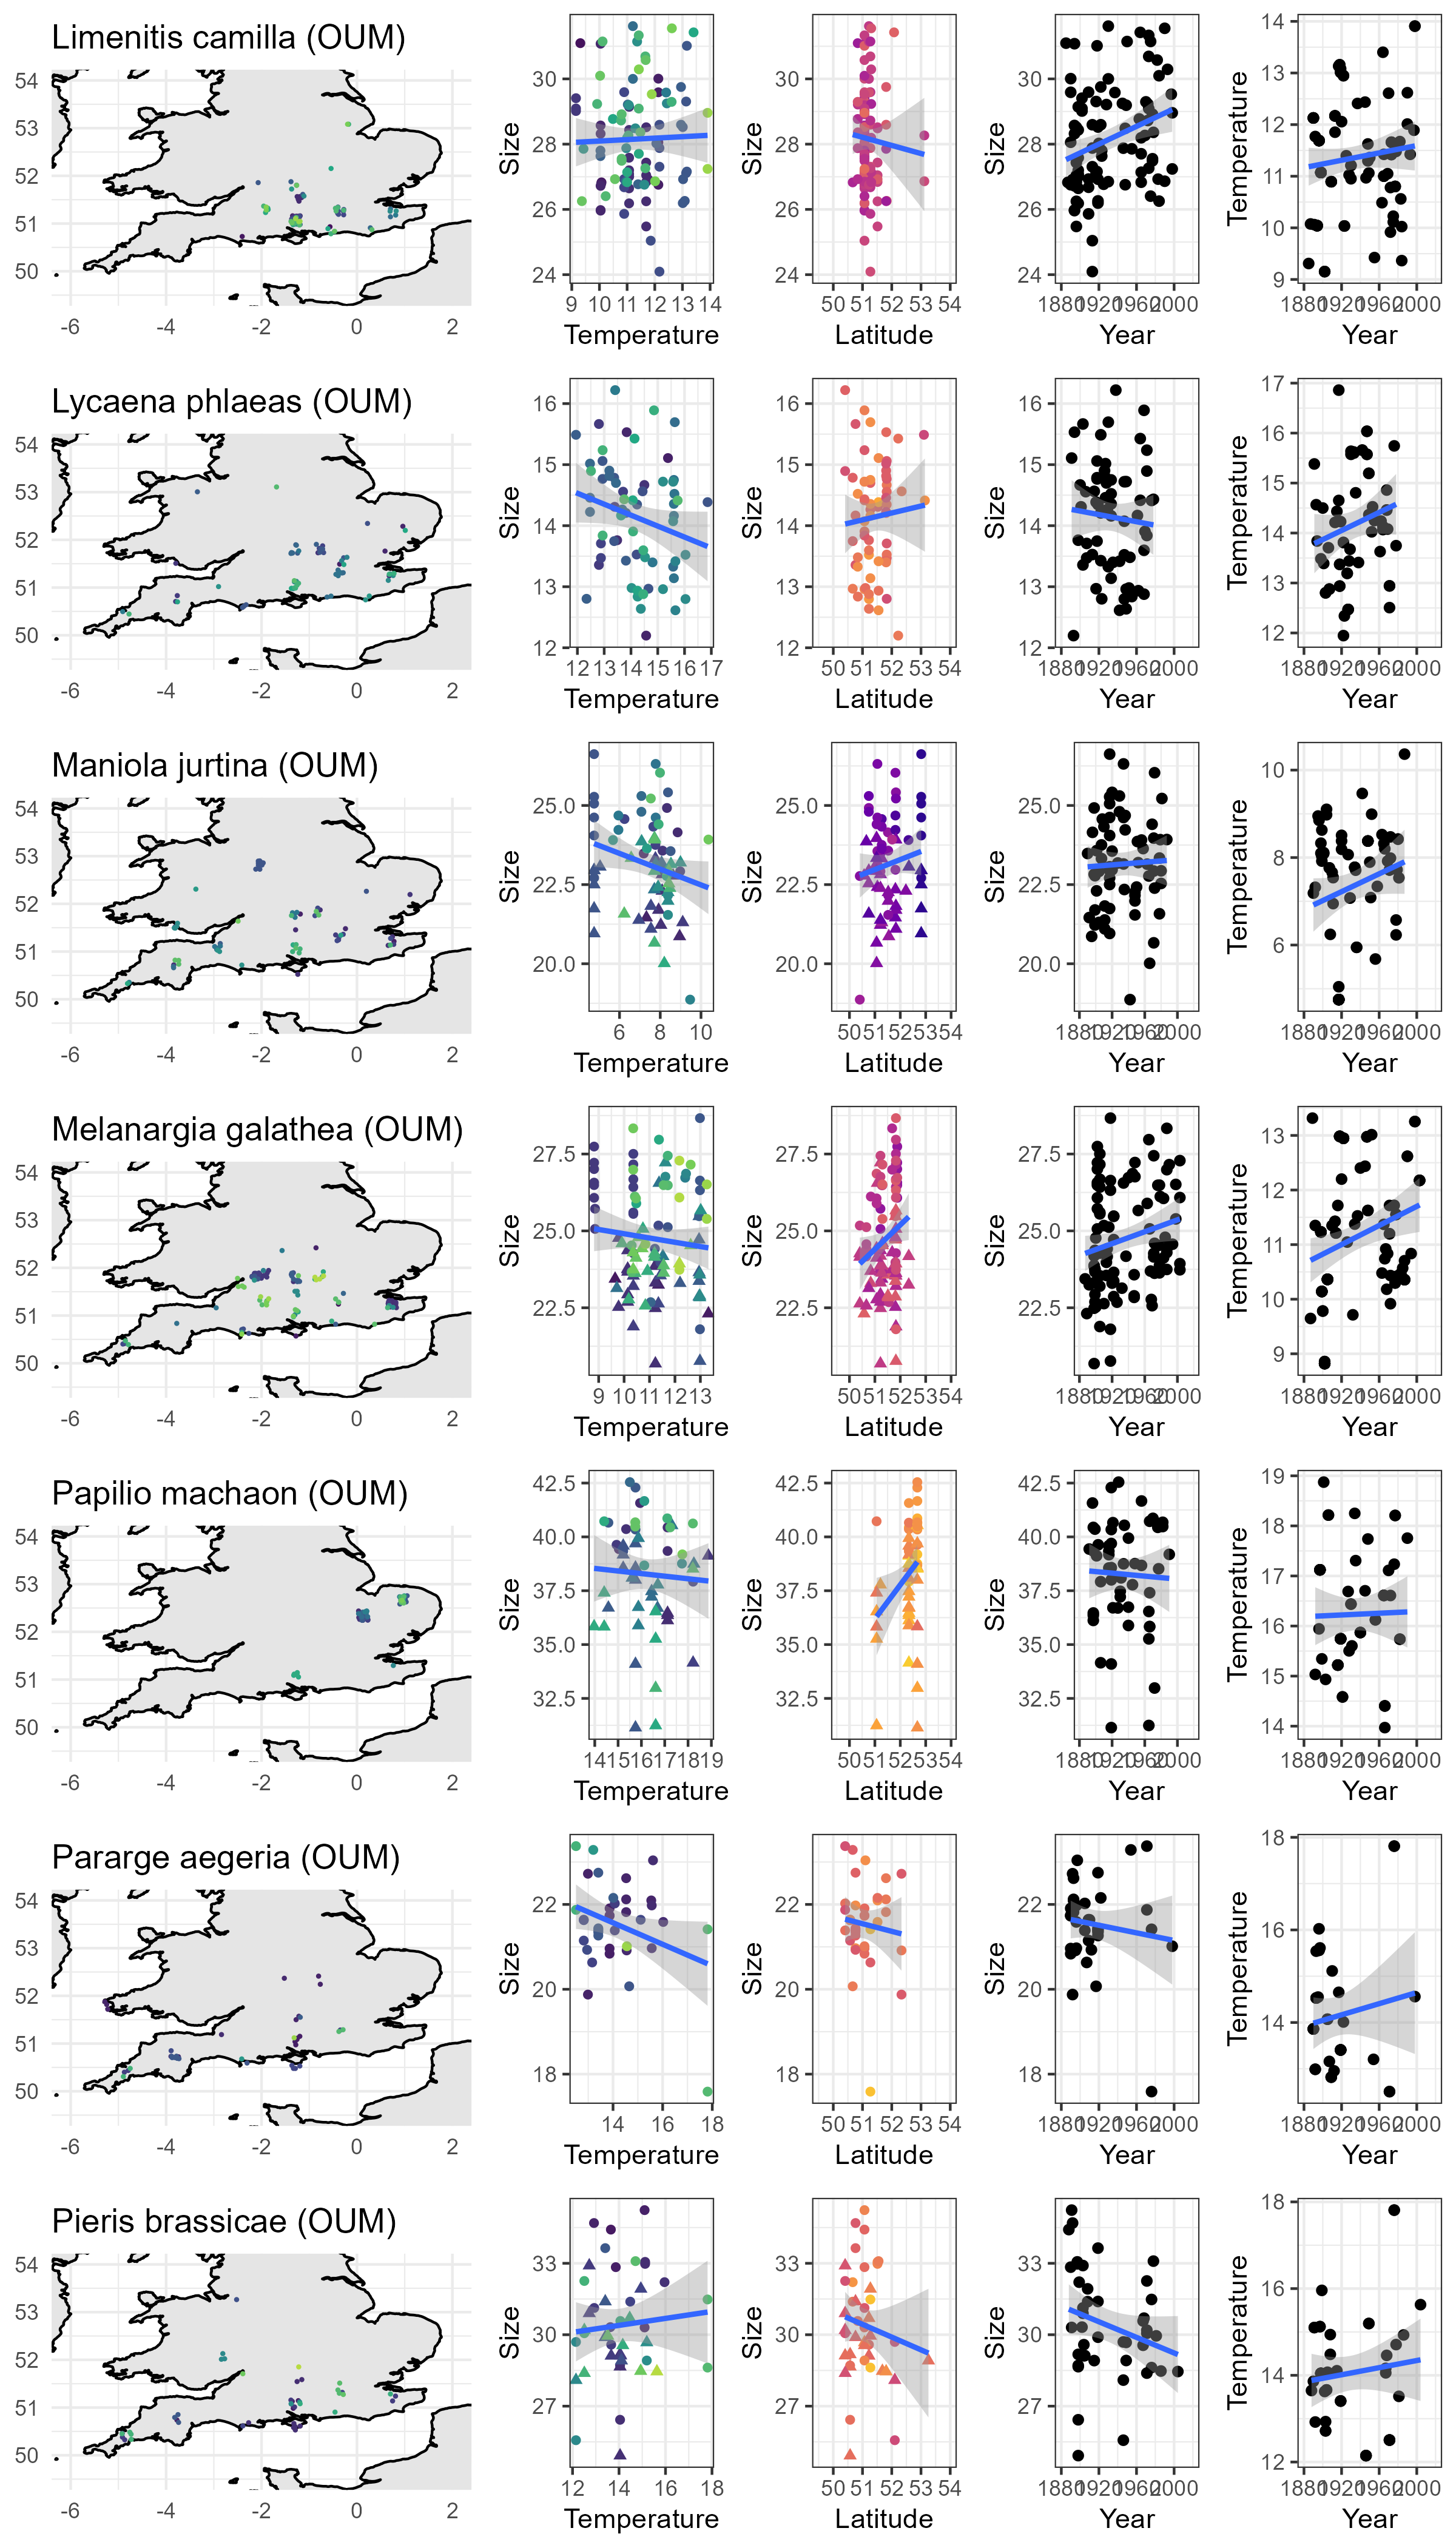
\includegraphics[width=\linewidth]{../figs/SI_OUM_dataspread_3.png}
\end{figure}
\begin{figure}[H]
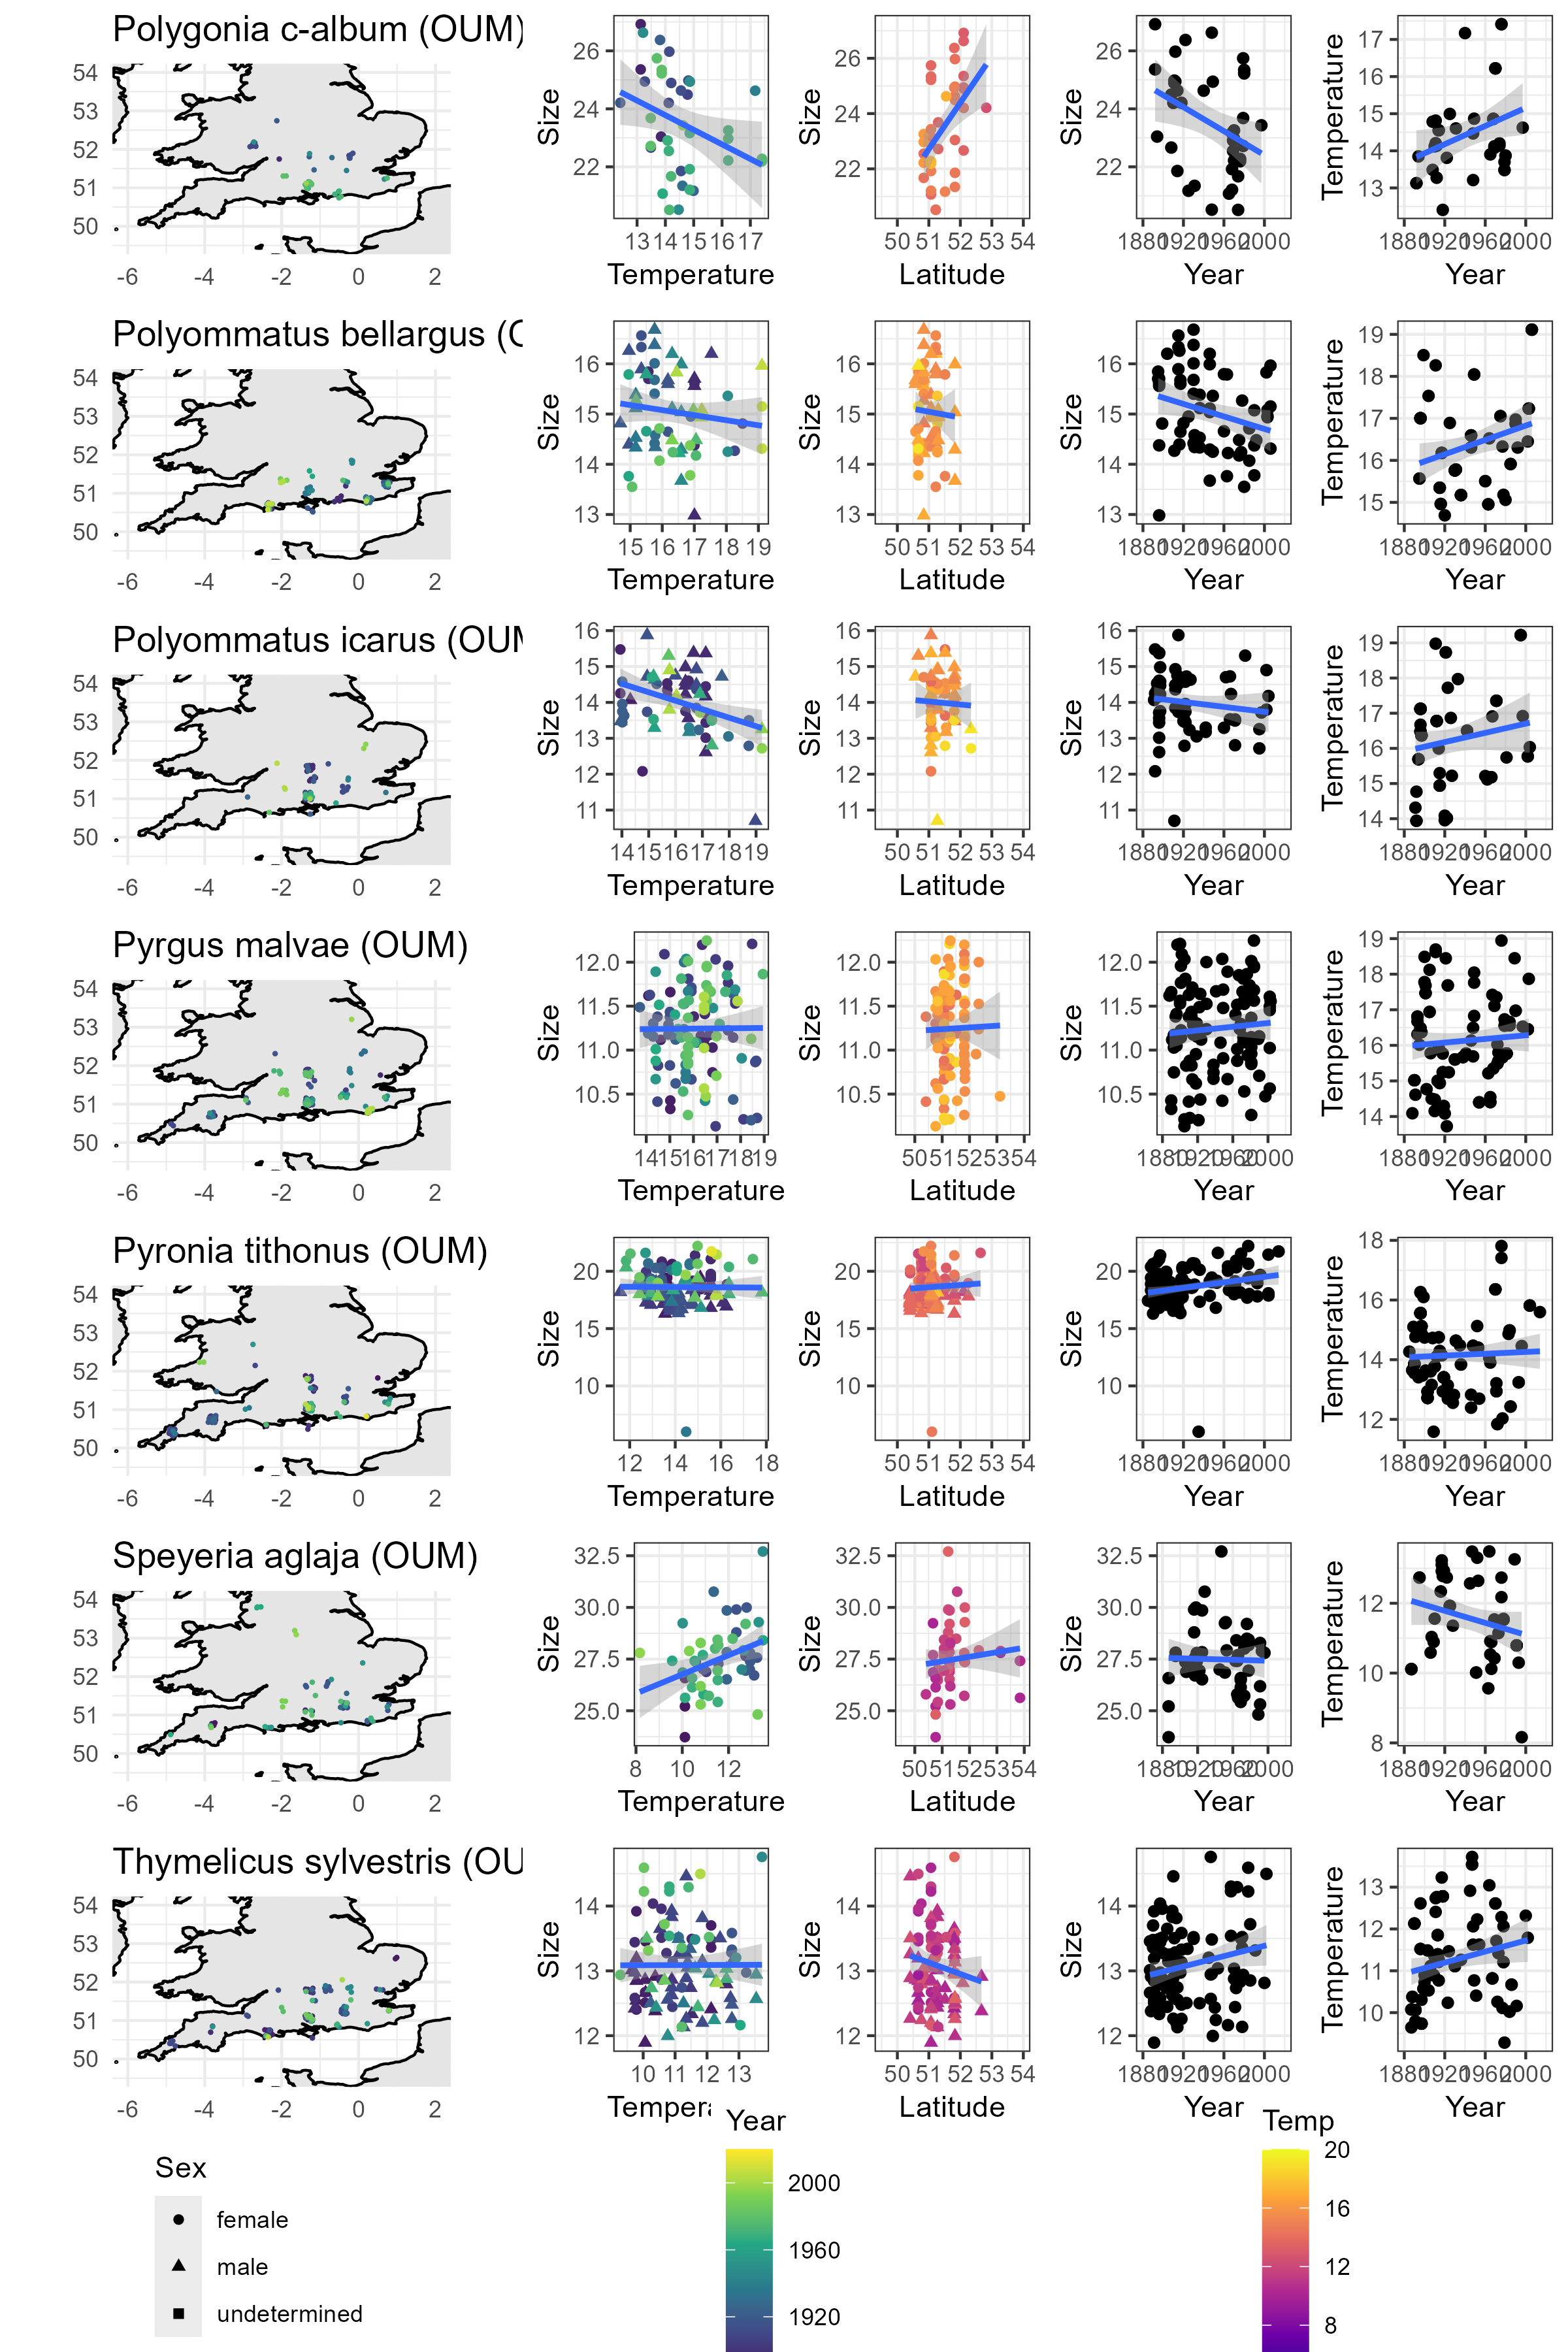
\includegraphics[width=\linewidth]{../figs/SI_OUM_dataspread_4.png}
\end{figure}

\textbf{Figure S11: Distribution of records (post-filtering) from the NHM dataset for each species} NB Locations on the map have been slightly jittered to reduce overlap. 



\end{document}